\documentclass[
  compress
  ,handout
  ,12pt
]{beamer}
%\usepackage[bookmarks=true,colorlinks=true,linkcolor=black,filecolor=blue,pagecolor=black,urlcolor=black]{hyperref}
\usepackage{amsmath}
\usepackage{amssymb}

\usepackage{mathrsfs}

\usetheme{Darmstadt}
\usecolortheme{sidebartab}
%\usecolortheme{rose}
\usepackage{times}
\usepackage{units}

\usepackage{mathrsfs}
%\usepackage{diss}

\usepackage{subfigure}

\usefonttheme[onlymath]{serif}

\author{Roy Stogner \\ \texttt{\tiny roystgnr@cfdlab.ae.utexas.edu}}
\institute[UT]
{
  \inst{1}Univ.\ of Texas at Austin
}

%{Computational Fluid Dynamics Lab
%\\ Institute for Computational Engineering and Sciences
%\\ University of Texas at Austin}
\date{March 31, 2008}

\logo{
\includegraphics[width=.5in]{figs/cfdlab}}

\begin{document}

\newcommand{\royslide}[2]{\frame{ \frametitle{#1} #2 }}
\newcommand{\royitemizebegin}[1]{\begin{block}{#1} \begin{itemize}}
\newcommand{\royitemizeend}{\end{itemize} \end{block}}

%\documentclass[landscape,pdftex,headrule,footrule]{foils}
\usepackage[bookmarks=true,colorlinks=true,linkcolor=black,filecolor=blue,pagecolor=black,urlcolor=black]{hyperref}
\usepackage{amsmath}
\usepackage{amssymb}
\usepackage[pdftex]{graphicx}
\usepackage{color}
\usepackage{url}
%\usepackage{citesort}
\usepackage{billfoiltex}
\usepackage{soul}
\usepackage[display,coloremph,colormath]{texpower}
\usepackage{verbatim}
\usepackage{layout}


\setlength\textheight{7.25in}
\setlength\textwidth{9.5in}
\setlength\oddsidemargin{-.25in}
\setlength\marginparwidth{.5in}
\setlength\topmargin{-.75in}
\setlength\headheight{.75in}
\setlength\headsep{-.4in}
\setlength\footskip{.4in}
\setlength\foilheadskip{0in}



%\renewcommand{\labelitemii}{\color{red}{$\rightarrow$}}
%\renewcommand{\labelitemiii}{\color{black}{$\boldsymbol{\cdot}$}}

\newlength{\sizewidelen}
% This makes the normal text version spaced equivalently to the bold face
% version.. Needed for highlighting to work nicely.
\newcommand{\sizewide}[1]{\settowidth{\sizewidelen}{{\bf #1}}\makebox[\sizewidelen][l]{#1}}
% Only display on the first step. 
\newcommand{\FirstOnly}[2]{\switch{#1}{\ifthenelse{\boolean{firstactivation}}{#2}{#1}}}
% Provides a List with descriptions \Firstonly{Header}{Description} that
% will be cycled through.
\newcommand{\ProgressItem}[2]{\FirstOnly{\textcolor[rgb]{0.5,0.5,0.5}{\sizewide{#1}}}{{\color{red}{#1}}\\{\color{black}#2}}}
% Simpler to \ProgressItem but ensures the "correct" amount of space
% after each item so that nothing moves between steps
% ( This command used to use phantom but it never worked correctly... )
\newcommand{\PIWPhant}[2]{\FirstOnly{\textcolor[rgb]{0.5,0.5,0.5}{\sizewide{#1}}\\\textcolor{pagecolor}{#2}}{{\color{red}{\bf #1}}\\{\color{black}#2}}}
\DeclareRobustCommand{\Cpp}{\hbox{\textsf{C\kern-.1em}\raise.3ex\hbox{\tiny{+}}\raise.3ex\hbox{\tiny{+}}}}


\author{\vspace{0.25in} \\ Roy Stogner
\vspace{0.25in} \\ Computational Fluid Dynamics Lab
\vspace{0.25in} \\ Institute for Computational Engineering and Sciences
\vspace{0.25in} \\ University of Texas at Austin}
\date{\vspace{.75in} December, 2006}
\hyperbaseurl{http://cfdlab.ae.utexas.edu/~roystgnr}
\MyLogo{\href{http://cfdlab.ae.utexas.edu/~roystgnr}{\texttt{roystgnr@cfdlab.ae.utexas.edu}}}

\leftheader{\href{http://cfdlab.ae.utexas.edu}{
\includegraphics[height=\headheight]{figs/cfdlab}}}
%\rightheader{\large{FEF05}}
%\rightheader{\includegraphics[height=\headheight]{figs/box_v}}
\rightheader{}
\rightfooter{\thepage}

\newcommand{\tightlist}{\itemsep=-1pt }


\input format5

\begin{document}
\raggedright
%\layout

\newcommand{\royslide}[2]{\begin{foil}{#1} #2 \end{foil}}
\newcommand{\royitemizebegin}{\begin{itemize}}
\newcommand{\royitemizeend}{\end{itemize}}




\newcommand{\refeq}[1]{(\ref{eq:#1})}
\newcommand{\refminor}[1]{Section \ref{minor:#1}}

\newcommand{\cpp}{C{\tiny$^{++}$}}

%\newcommand{\libMesh}{\href{http://libmesh.sourceforge.net}{\texttt{libMesh}}}
%\newcommand{\CFDLab}{\href{http://cfdlab.ae.utexas.edu}{CFDLab}}
%\newcommand{\PETSc}{\href{http://www-unix.mcs.anl.gov/petsc/petsc-2}{PETSc}}
\newcommand{\libMesh}{\texttt{lib\-Mesh}}
\newcommand{\CFDLab}{CFDLab}
\newcommand{\PETSc}{PETSc}

\newcommand{\abs}[1]{\ensuremath{ \left| #1 \right| }}
\newcommand{\commentout}[1]{}
\newcommand{\dn}[1]{\ensuremath{\partial_{\vec{n}} #1}}
\newcommand{\dns}[1]{\ensuremath{\partial_{\vec{n_S}} #1}}
\newcommand{\ds}[1]{\ensuremath{\partial_{\vec{s}} #1}}
%\newcommand{\dn}[1]{\ensuremath{dn #1}}
%\newcommand{\ds}[1]{\ensuremath{ds #1}}
\newcommand{\dt}[1]{\ensuremath{\frac{\partial #1}{\partial t}}}
\newcommand{\dx}[1]{\ensuremath{\partial_x #1}}
\newcommand{\dy}[1]{\ensuremath{\partial_y #1}}
%\newcommand{\dx}[1]{\frac{\partial #1}{\partial x}}
%\newcommand{\dy}[1]{\frac{\partial #1}{\partial y}}
\newcommand{\dT}[1]{\ensuremath{\frac{\partial}{\partial t}\left(#1\right)}}
\newcommand{\dX}[1]{\ensuremath{\frac{\partial}{\partial x}\left(#1\right)}}
\newcommand{\dY}[1]{\ensuremath{\frac{\partial}{\partial y}\left(#1\right)}}
\newcommand{\norm}[1]{\ensuremath{ \left|\left| #1 \right|\right| }}
\newcommand{\jump}[1]{\ensuremath{ \left[\hspace{-0.1em}\left[ #1 
                      \right]\hspace{-0.1em}\right] }}
\newcommand{\partials}[2]{\ensuremath{\frac{\partial #1}{\partial #2}}}
\newcommand{\vorticity}{\ensuremath{\omega}}
\newcommand{\vu}{\ensuremath{\vec{u}}}
\newcommand{\vun}{\ensuremath{\vec{u}^{(n)}}}
\newcommand{\vup}{\ensuremath{\vec{u}^{(n+1)}}}
\newcommand{\vud}{\ensuremath{\delta \vec{u}}}
\newcommand{\GDA}{\ensuremath{{\Gamma_{D1}}}}
\newcommand{\GDB}{\ensuremath{{\Gamma_{D2}}}}
\newcommand{\GNA}{\ensuremath{{\Gamma_{N1}}}}
\newcommand{\GNB}{\ensuremath{{\Gamma_{N2}}}}
\newcommand{\Reals}{\mathbb{R}}

\newcommand{\un}{\ensuremath{u^{(n)}}}
\newcommand{\up}{\ensuremath{u^{(n+1)}}}
\newcommand{\ut}{\ensuremath{u^{(\theta)}}}
\newcommand{\utb}{\ensuremath{\bar{u}^{(\theta)}}}
\newcommand{\uhn}{\ensuremath{u_h^{(n)}}}
\newcommand{\uhp}{\ensuremath{u_h^{(n+1)}}}
\newcommand{\uht}{\ensuremath{u_h^{(\theta)}}}
\newcommand{\ehn}{\ensuremath{e_h^{(n)}}}
\newcommand{\ehp}{\ensuremath{e_h^{(n+1)}}}
\newcommand{\eht}{\ensuremath{e_h^{(\theta)}}}
\newcommand{\ePn}{\ensuremath{e_P^{(n)}}}
\newcommand{\ePp}{\ensuremath{e_P^{(n+1)}}}
\newcommand{\ePt}{\ensuremath{e_P^{(\theta)}}}
\newcommand{\ePtb}{\ensuremath{\bar{e}_P^{(\theta)}}}

\newcommand{\Laplacian}{\Delta}
\newcommand{\Biharmonic}{\Delta^2}

\newcommand{\D}{\delta}

\newcommand{\Biot}{\ensuremath{ {\rm H}}}
\newcommand{\Galileo}{\ensuremath{ {\rm G}}}
\newcommand{\Marangoni}{\ensuremath{ {\rm M}}}
\newcommand{\Prandtl}{\ensuremath{ {\rm Pr}}}
\newcommand{\Raleigh}{\ensuremath{ {\rm Ra}}}
\newcommand{\Reynolds}{\ensuremath{ {\rm Re}}}
\newcommand{\ReMax}{\ensuremath{ \Reynolds_{{\rm max}}}}

\newcommand{\height}{\ensuremath{u}}
\newcommand{\dheight}{\ensuremath{v}}
\newcommand{\surf}{\ensuremath{c_s}}
\newcommand{\dsurf}{\ensuremath{w}}

\newcommand{\penaltyeps}{\ensuremath{\epsilon}}

\newcommand{\ex}{\hat{e}_x}
\newcommand{\ey}{\hat{e}_y}
\newcommand{\ez}{\hat{e}_z}

\newcommand{\R}{\mathscr{R}}



\title{libMesh Finite Element Library}
%\maketitle

\begin{frame}
  \titlepage
  \begin{picture}(100,100)
    \put(0,150){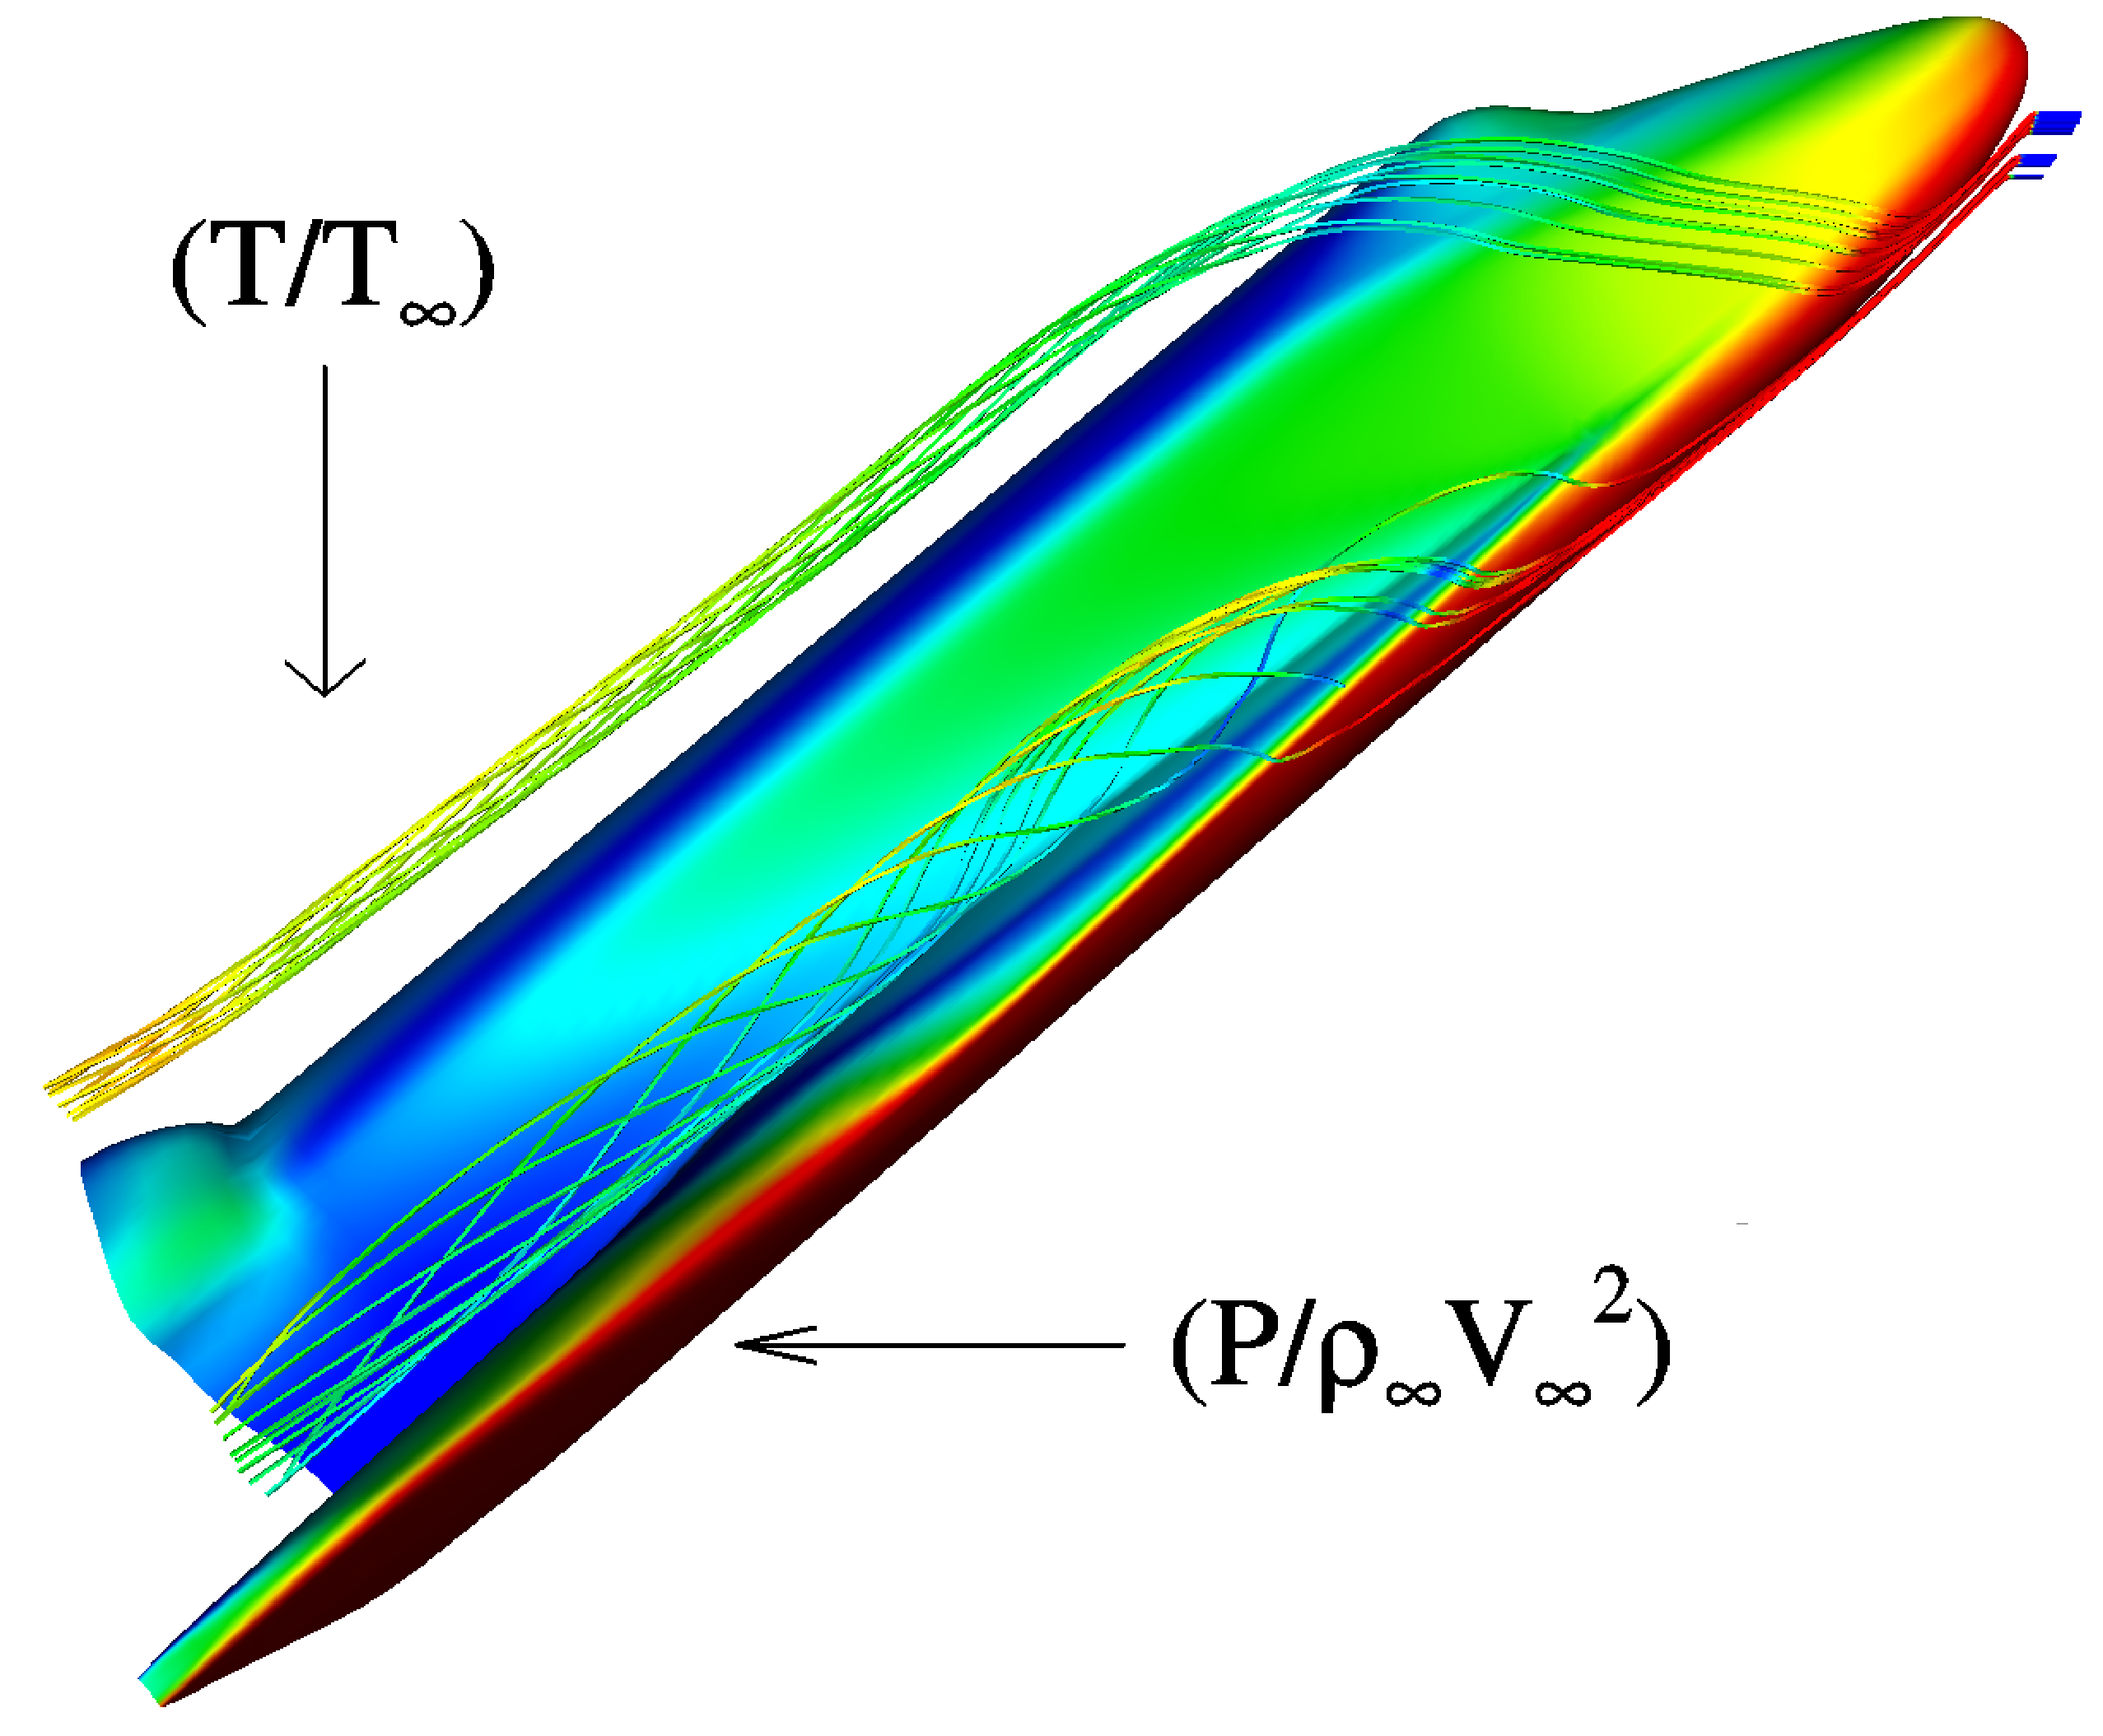
\includegraphics[viewport=0 0 470 400,clip=true,width=.3\textwidth]{figs/Benkirk_orbiter_reentry_side_view}}
    \put(220,150){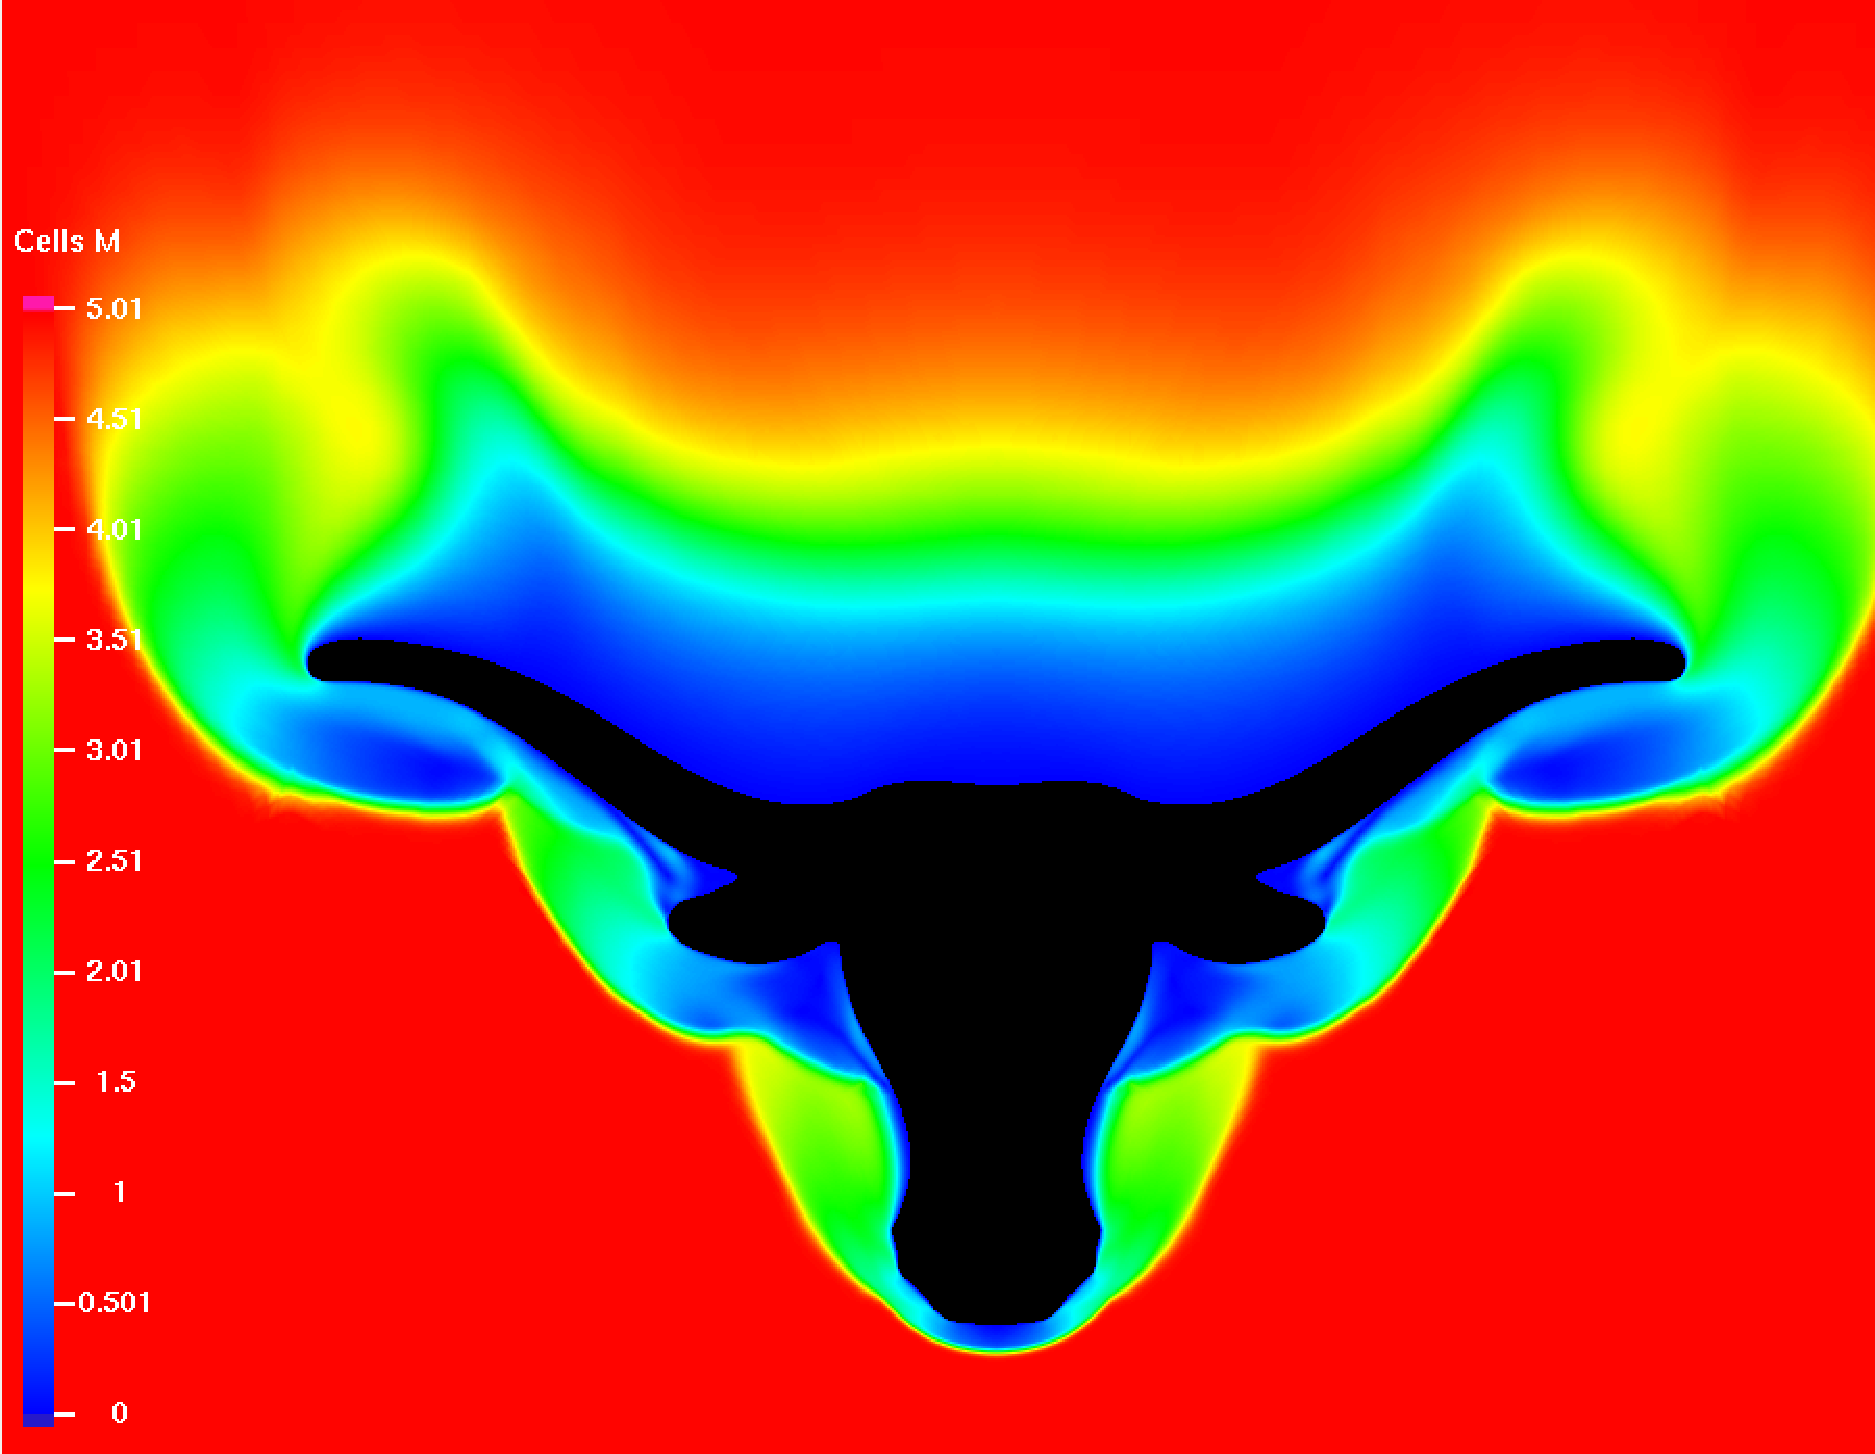
\includegraphics[viewport=0 0 350 300,clip=true,width=.3\textwidth]{figs/Hypersonic_cow_mach}}
  \end{picture}
\end{frame}

\section*{Outline}% Make it easy to jump to this page in the PDF

% use outline_currentsection.tex to highlight the current section

% Auto-generate the TOC slide(s)
\begin{frame}
  %\tableofcontents[currentsection]
  \tableofcontents
\end{frame}






% The optional argument [<+->] means everything on the frame will be displayed incrementally.
\section{Introduction}
% Auto-generate the TOC slide(s)
\begin{frame}
  \tableofcontents[currentsection]
  %\tableofcontents
\end{frame}

\subsection{Acknowledgments}
\begin{frame}[shrink]
  \begin{block}{Code Contributors}
    \scriptsize
    \begin{center}
      \begin{tabular}{|l|l|} \hline
        Benjamin S. Kirk & benkirk \\
        Bill Barth       & bbarth \\
        Cody Permann     & permcody \\
        Daniel Dreyer    & ddreyer \\
        David Andrs      & andrsd \\
        David Knezevic   & knezed01 \\
        Derek Gaston     & friedmud \\
        Dmitry Karpeev   & karpeev \\
        Florian Prill    & fprill \\
        Jason Hales      & jasondhales \\
        John W. Peterson & jwpeterson \\
        Paul T. Bauman   & pbauman \\
        Roy H. Stogner   & roystgnr \\
        Steffen Petersen & spetersen \\
        Sylvain Vallaghe & svallagh \\
        Tim Kroeger      & sheep\_tk \\
        Truman Ellis     & trumanellis \\
        Wout Ruijter     & woutruijter \\ \hline
      \end{tabular}
    \end{center}
    \begin{itemize}
      \item Thanks to Wolfgang Bangerth and the \texttt{deal.II} team for initial technical inspiration. 
      \item Also, thanks to Jed Brown, Robert McLay, \& many others for discussions over the years.
    \end{itemize}
  \end{block}
\end{frame}

\frame
{
  \frametitle{Thanks to Dr.\ Graham F.\ Carey}

  \begin{columns}
    \begin{column}{.55\textwidth}
      \scriptsize
      \begin{quote}
        The original development team was heavily influenced by Professor Graham F. Carey, professor of aerospace engineering and engineering mechanics at The University of Texas at Austin, director of the ICES Computational Fluid Dynamics Laboratory, and holder of the Richard B. Curran Chair in Engineering.

        Many of the technologies employed in libMesh were implemented because Dr. Carey taught them to us, we went back to the lab, and immediately began coding. In a very real way, he was ultimately responsible for this library that we hope you may find useful, despite his continued insistence that ``no one ever got a PhD from here for writing a code.''       
      \end{quote}
\normalsize
    \end{column}
    \begin{column}{.45\textwidth}
      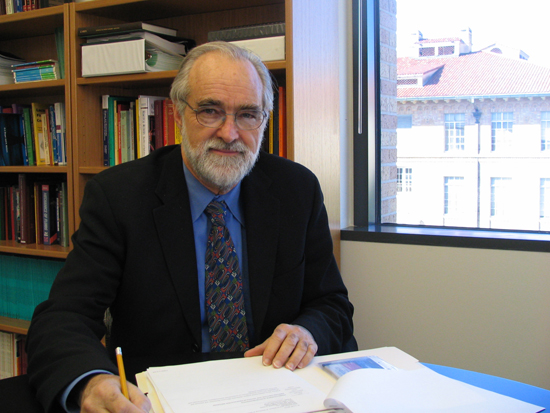
\includegraphics[width=\textwidth]{grahamcarey}
    \end{column}
  \end{columns}
}

\subsection{Background}
%%%%%%%%%%%%%%%%%%%%%%%%%%%%%%%%%%%%%%%%%%%%%%%%%
\frame
{
  \frametitle{Background}                 

  \begin{itemize}
  \item Modern simulation software is \emphcolor{complex}:
    \begin{itemize}
    \item Implicit numerical methods
    \item Massively parallel computers
    \item Adaptive methods
    \item Multiple, coupled physical processes
    \end{itemize}
    %\pause
  \item There are a host of existing software libraries that excel at treating various aspects of this complexity.
  \item Leveraging existing software whenever possible is the most efficient way to manage this complexity.

  \end{itemize}
}


 

%%%%%%%%%%%%%%%%%%%%%%%%%%%%%%%%%%%%%%%%%%%%%%%%%
\frame
{
  \frametitle{Background}                 

  \begin{itemize}
  \item Modern simulation software is \emphcolor{multidisciplinary}:
    \begin{itemize}
    \item Physical Sciences
    \item Engineering
    \item Computer Science
    \item Applied Mathematics
    \item \ldots
    \end{itemize}
  \item It is not reasonable to expect a single person to have all the necessary skills for developing \& implementing high-performance numerical algorithms on modern computing architectures.
  \item Teaming is a prerequisite for success.
  \end{itemize}
}


 

%%%%%%%%%%%%%%%%%%%%%%%%%%%%%%%%%%%%%%%%%%%%%%%%%
\frame
{
  \frametitle{Background}                 
  \begin{itemize}
    \item A large class of problems are amenable to \emphcolor{mesh based} simulation techniques.
      %% \begin{columns}[t]
      %%   \column{.5\textwidth}        
      %%   \fbox{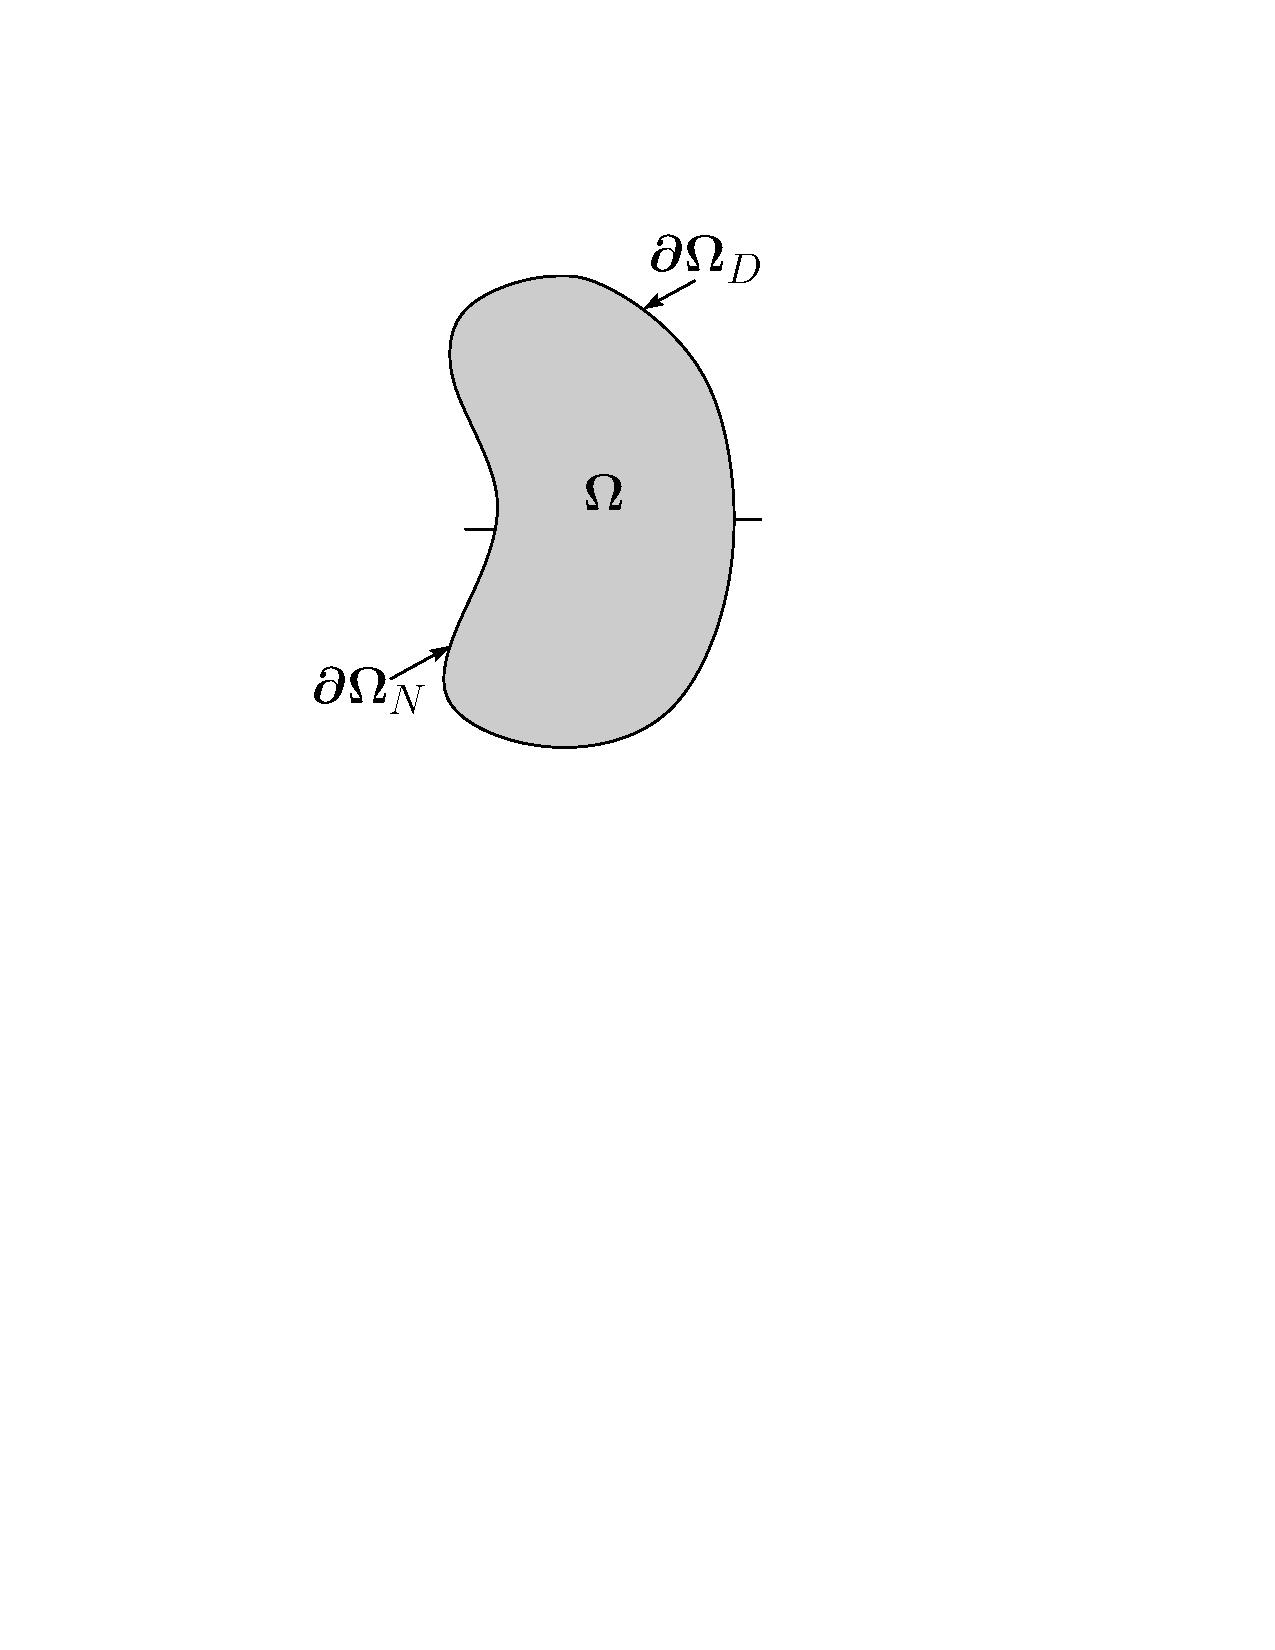
\includegraphics[viewport=140 420 400 685,clip=true,height=1in]{domain2/domain2_input}}
      %%   \column{.5\textwidth}
      %%   \fbox{\includegraphics[height=1in,angle=-90]{discretized_domain}}
      %% \end{columns}
    \item Consider some of the major components such a simulation:
      \pause
      \begin{enumerate}
        \item Read the mesh from file
        \item Initialize data structures
        \item Construct a discrete representation of the governing equations
        \item Solve the discrete system
        \item Write out results
        \item Optionally estimate error, refine the mesh, and repeat
      \end{enumerate}

    \pause
    \item With the exception of step 3, the rest is \emph{independent} of the class of problems being solved.
    \pause
    \item This allows the major components of such a simulation to be abstracted \& implemented in a reusable software library.
  \end{itemize}
}


 

\subsection{The \libmesh{} Software Library}
%%%%%%%%%%%%%%%%%%%%%%%%%%%%%%%%%%%%%%%%%%%%%%%%%
\frame
{
  \frametitle{The \libmesh{} Software Library}
  \begin{itemize}
    \item In 2002, the \libmesh{} library began with these ideas in mind.
    \item Primary goal is to provide data structures and algorithms that can be shared by disparate physical applications, that may need some combination of
      \begin{itemize}
      \item Implicit numerical methods
      \item Adaptive mesh refinement techniques
      \item Parallel computing
      \end{itemize}
    \item Unifying theme: \emphcolor{mesh-based simulation of partial differential equations (PDEs)}.
  \end{itemize}
}



 

\subsection{Software Reusability}
%%%%%%%%%%%%%%%%%%%%%%%%%%%%%%%%%%%%%%%%%%%%%%%%%
\frame
{
  \frametitle{The \libmesh{} Software Library}

  \begin{block}{Key Point}
    \begin{itemize}
      \item The \libmesh{} library is designed to be used by students, researchers, scientists, and engineers as a tool for \emphcolor{developing simulation codes} or as a tool for \emphcolor{rapidly implementing a numerical method}.
      \item \libMesh{} is not an application code.
      \item It does not ``solve problem XYZ.''
        \begin{itemize}
          \item It can be used to help you develop an application to solve problem XYZ, and to do so quickly with advanced numerical algorithms on high-performance computing platforms.
        \end{itemize}
      %\item It was initially targeted for finite element based simulations, but has been used for finite volume discretizations as well.
    \end{itemize}    
  \end{block}
} 



%%%%%%%%%%%%%%%%%%%%%%%%%%%%%%%%%%%%%%%%%%%%%%%%%
\frame
{
  \frametitle{Software Reusability}
  \begin{itemize}
    \item At the inception of \libMesh{} in 2002, there were many high-quality software libraries that implemented some aspect of the end-to-end PDE simulation process:
      \begin{itemize}
        \item Parallel linear algebra
        \item Partitioning algorithms for domain decomposition
        \item Visualization formats
        \item \ldots
      \end{itemize}
    \item A design goal of \libMesh{} has always been to provide flexible \& extensible interfaces to existing software whenever possible.
    \item We implement the ``glue'' to these pieces, as well as what we viewed as the missing infrastructure:
      \begin{itemize}
        \item \emphcolor{Flexible data structures for the discretization of spatial domains and systems of PDEs posed on these domains.}
      \end{itemize}          
  \end{itemize}  
}



%%%%%%%%%%%%%%%%%%%%%%%%%%%%%%%%%%%%%%%%%%%%%%%%%
\begin{frame}[t]
  %\frametitle{LibMesh Tree}
%  \vspace{-.25in}
%  \begin{center}
%    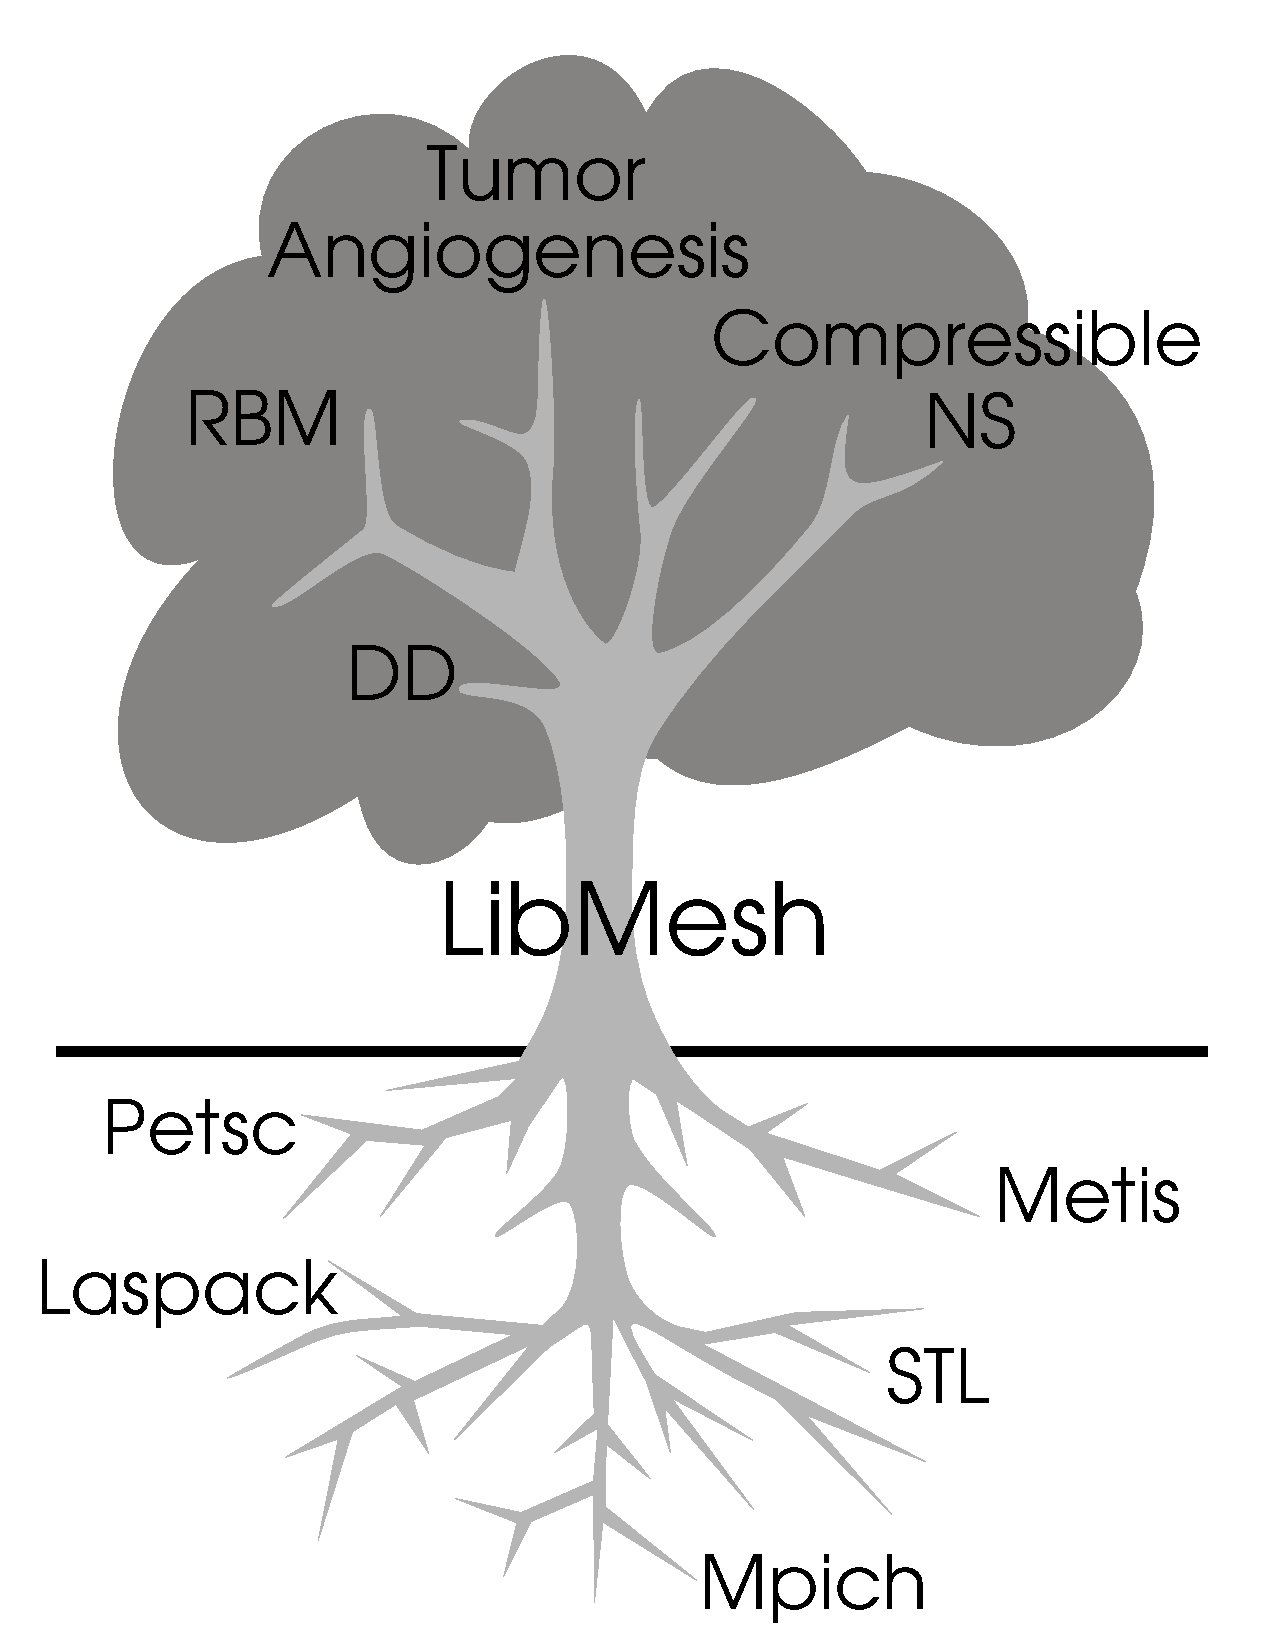
\includegraphics[width=.6\textwidth]{mytreeandroots_allnames}    
%  \end{center}


    \begin{minipage}[h]{.6\textwidth}
    \begin{center}
      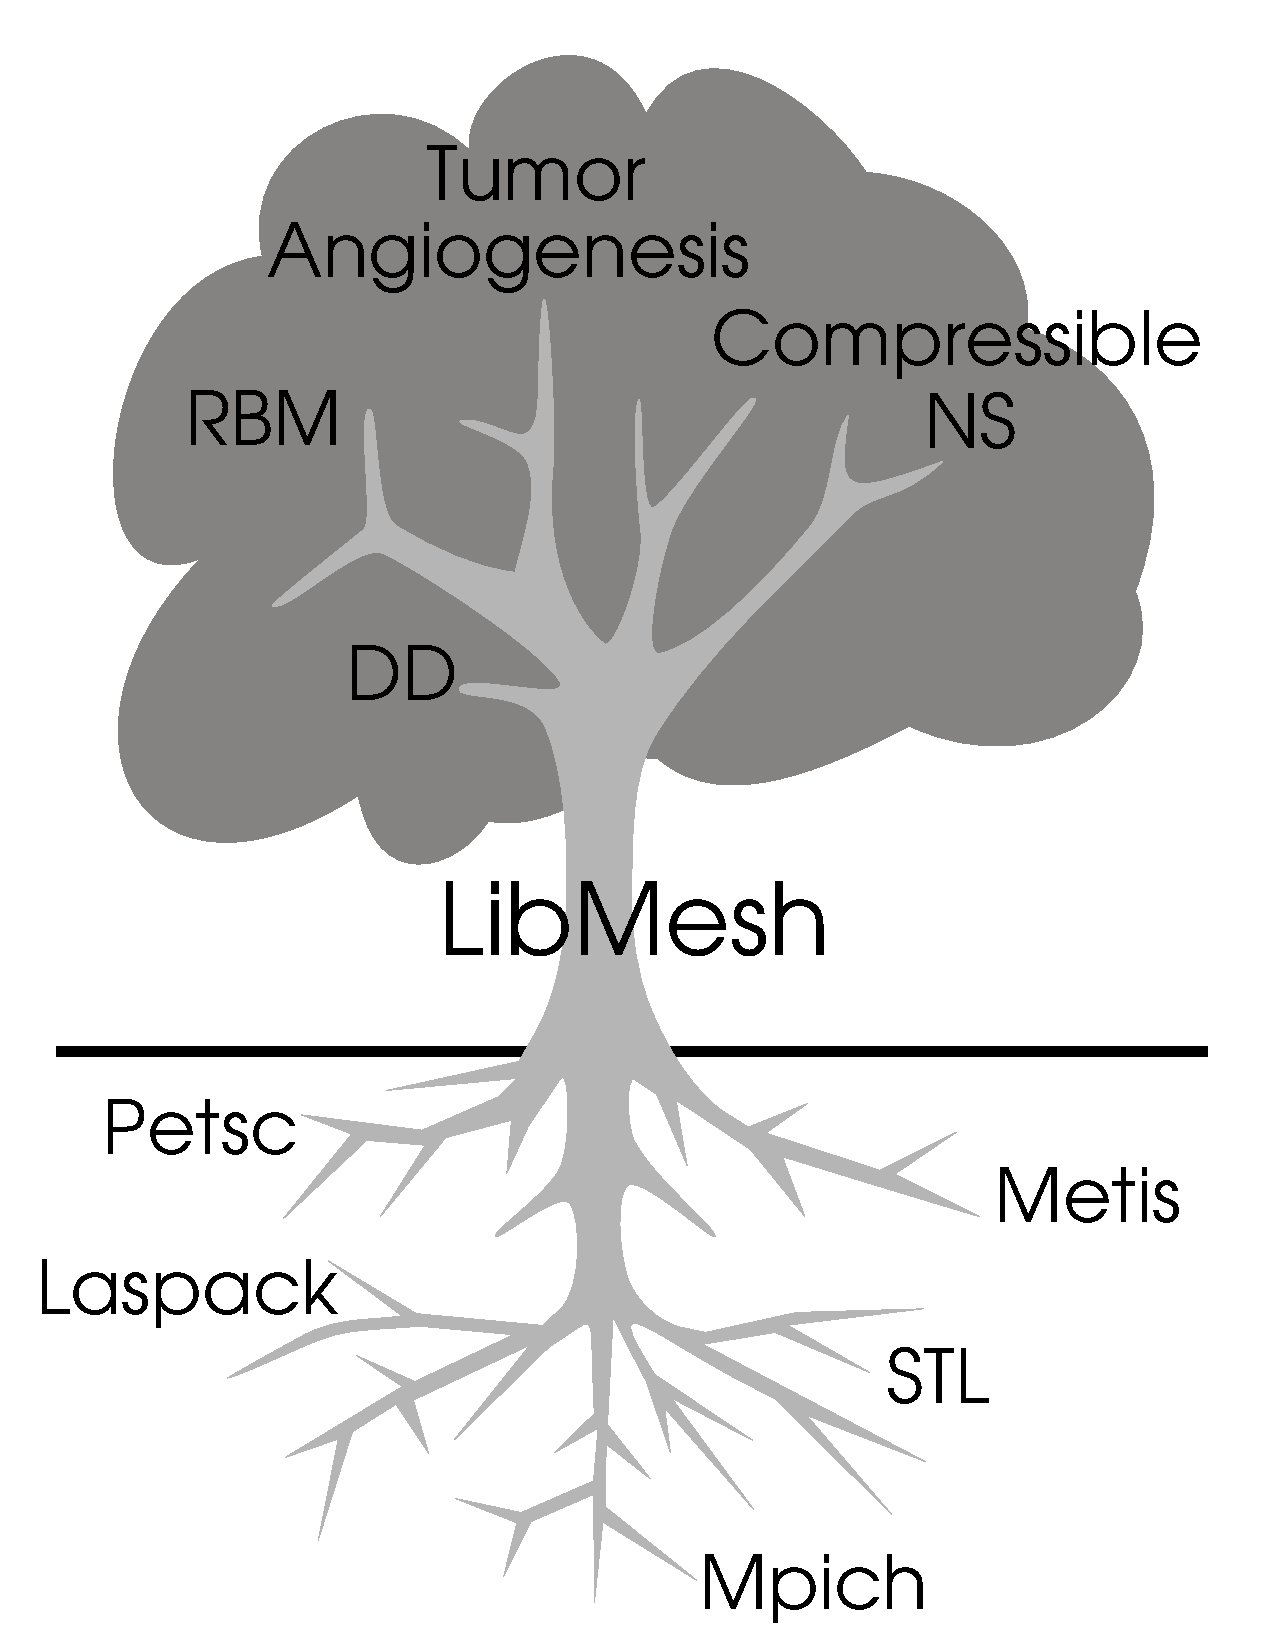
\includegraphics[width=.9\textwidth]{mytreeandroots_allnames}
    \end{center}
  \end{minipage}
  \begin{minipage}[h]{.35\textwidth}
    \begin{block}{Library Structure}
      \begin{itemize}
        %\small
    \item Basic libraries are \LibMesh's ``roots''
    \item Application ``branches'' built off the library ``trunk''
      \end{itemize}
    \end{block}
  \end{minipage}
\end{frame}


\subsection{Library Trivia}
\frame
{
  \frametitle{Trivia -- Downloads}
  \begin{center}
    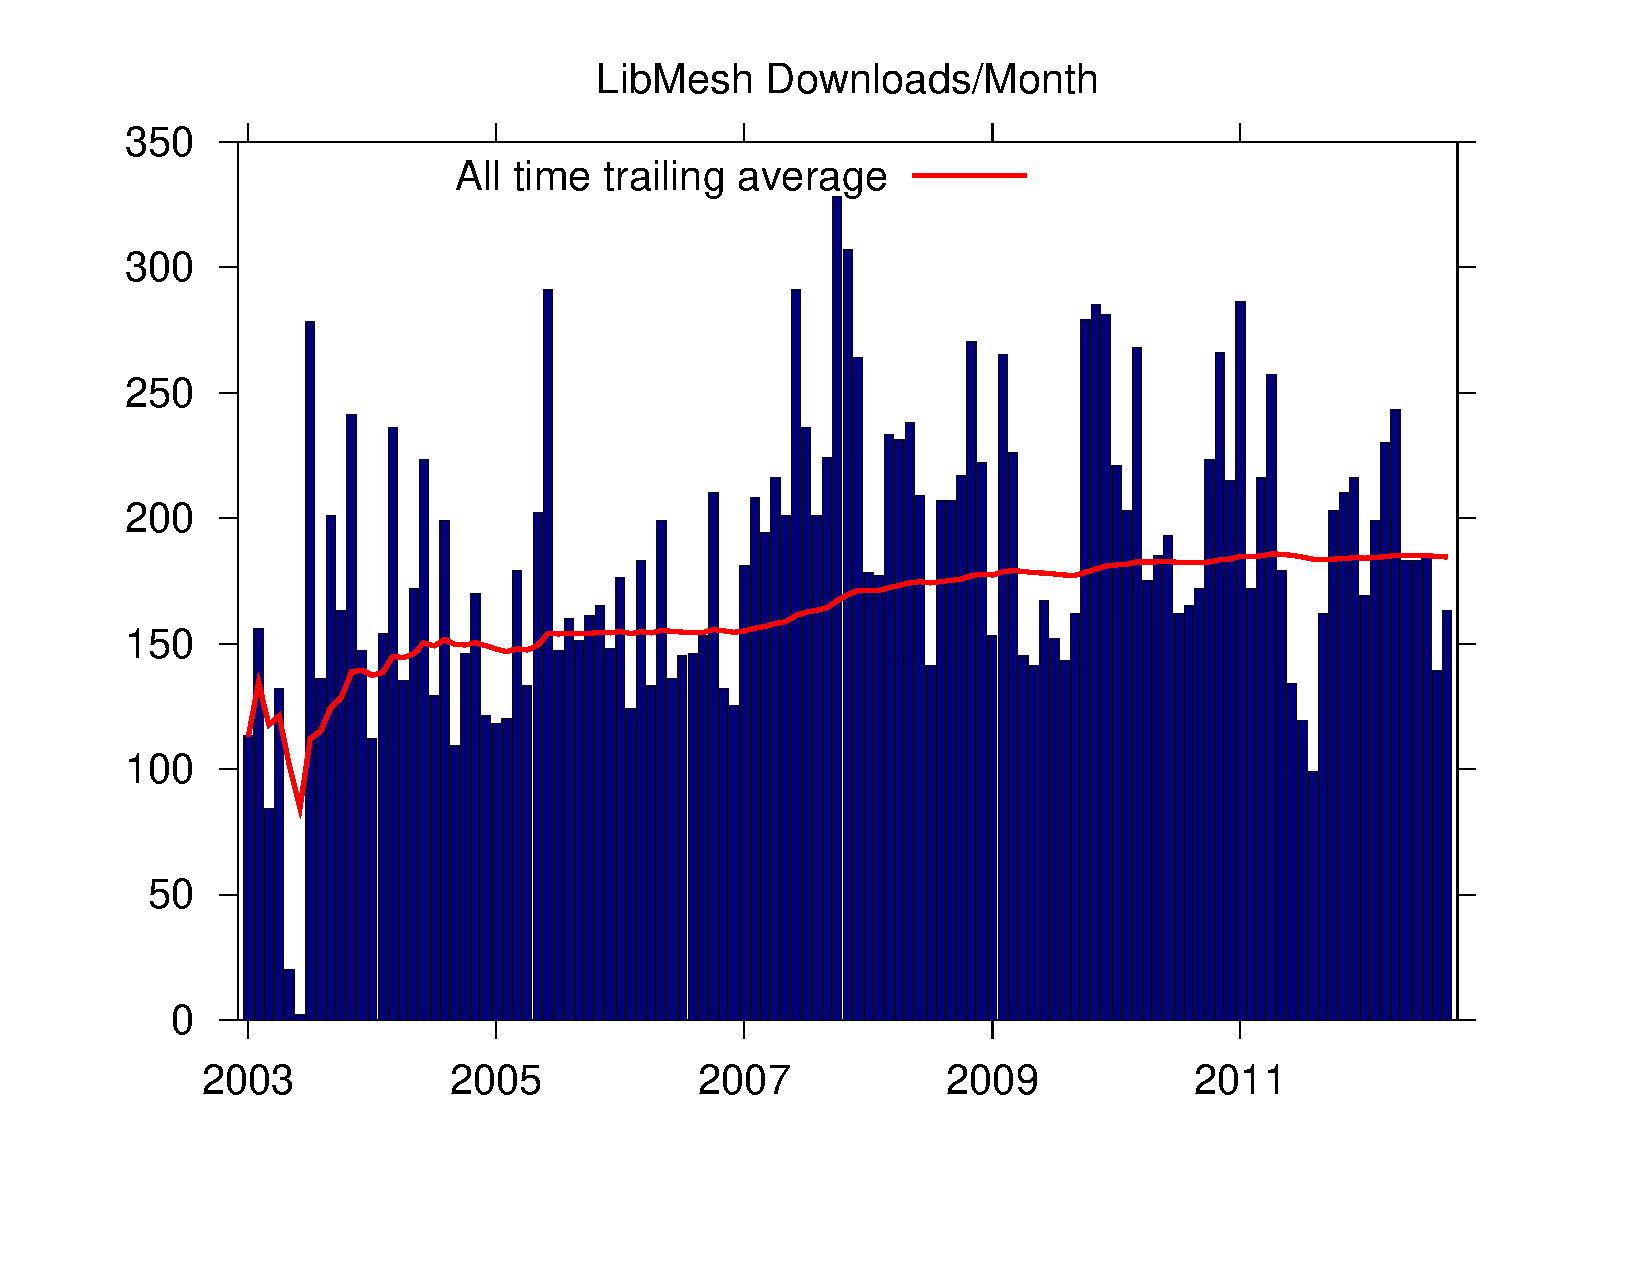
\includegraphics[height=0.8\textheight]{trivia/libmesh_downloads}
  \end{center}
}       

\frame
{
  \frametitle{Trivia -- Mailing List Membership}
  \begin{center}
    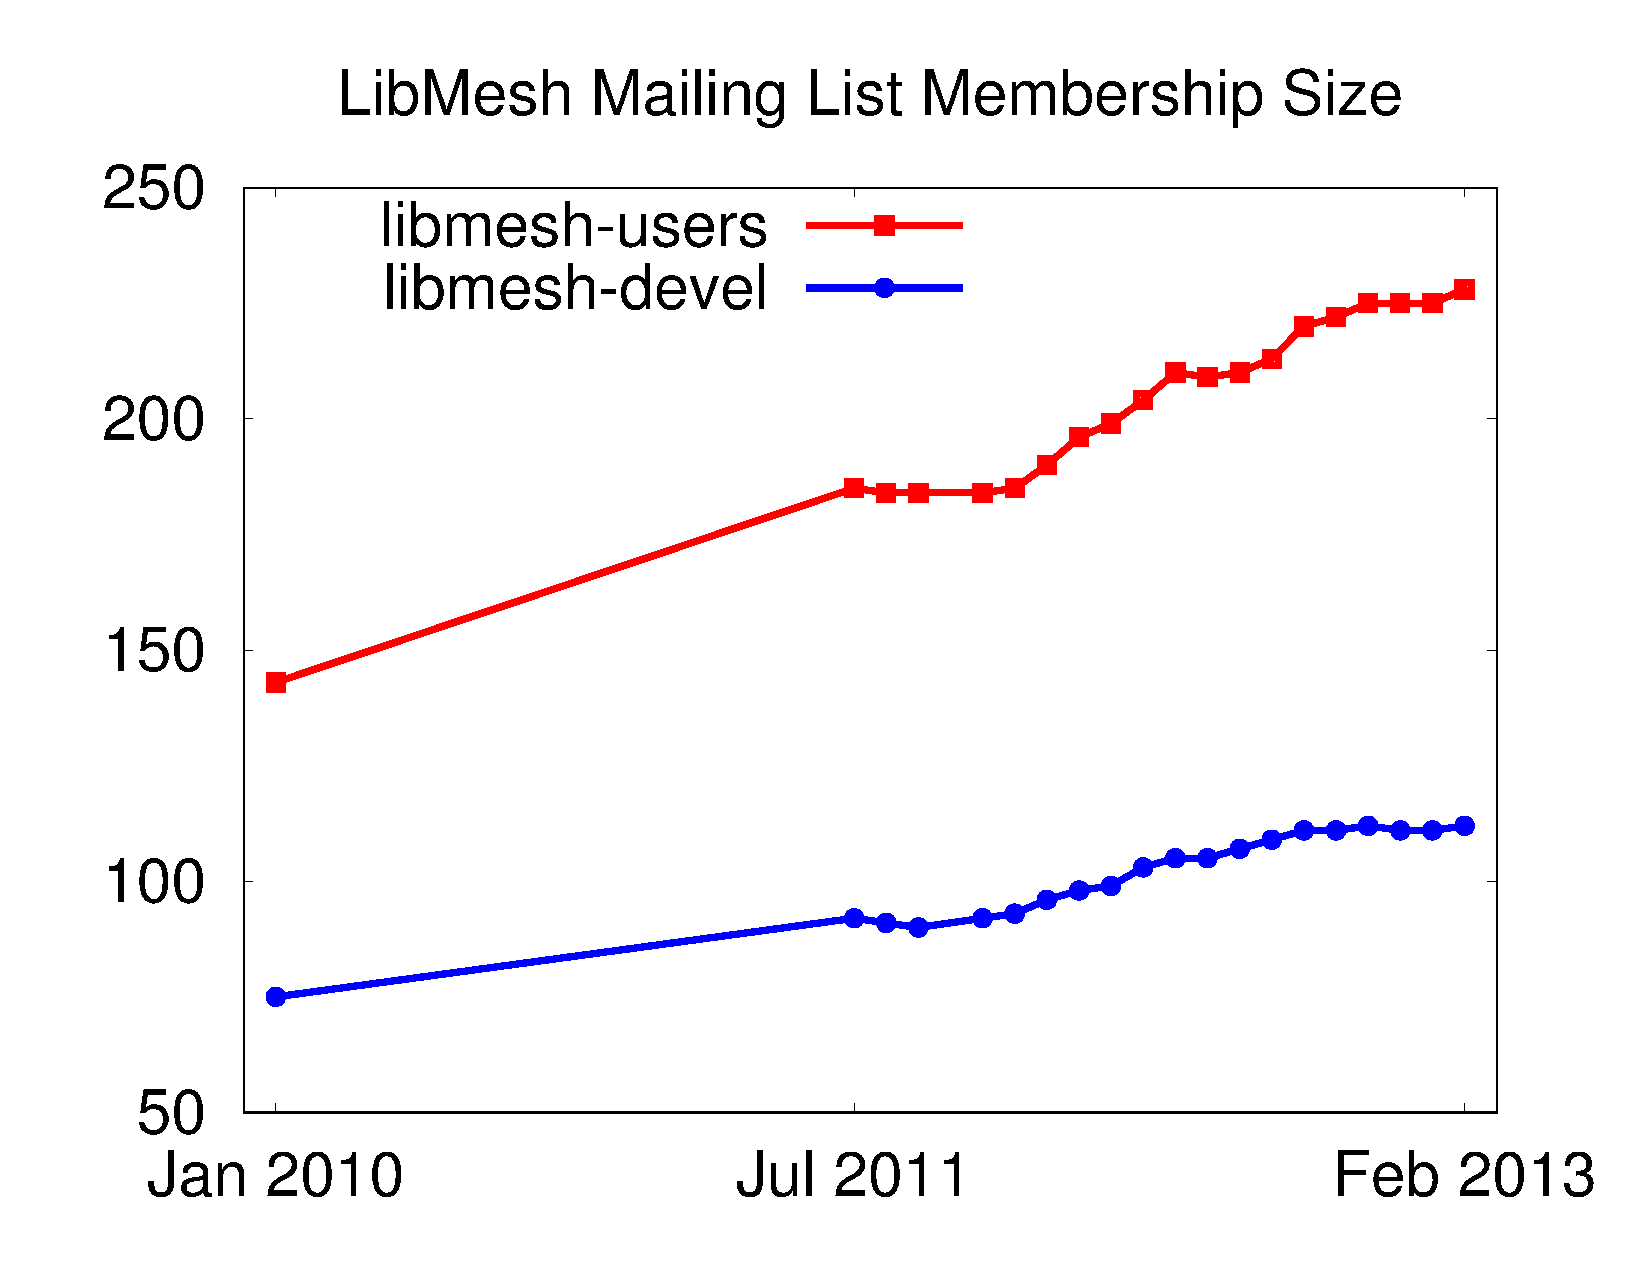
\includegraphics[height=0.8\textheight]{trivia/libmesh_mailinglists_membership}
    
    \small
    
    \url{libmesh-users@lists.sourceforge.net}

    \url{libmesh-devel@lists.sourceforge.net}
  \end{center}
}       

\frame
{
  \frametitle{Trivia -- Citations}
  \begin{center}
    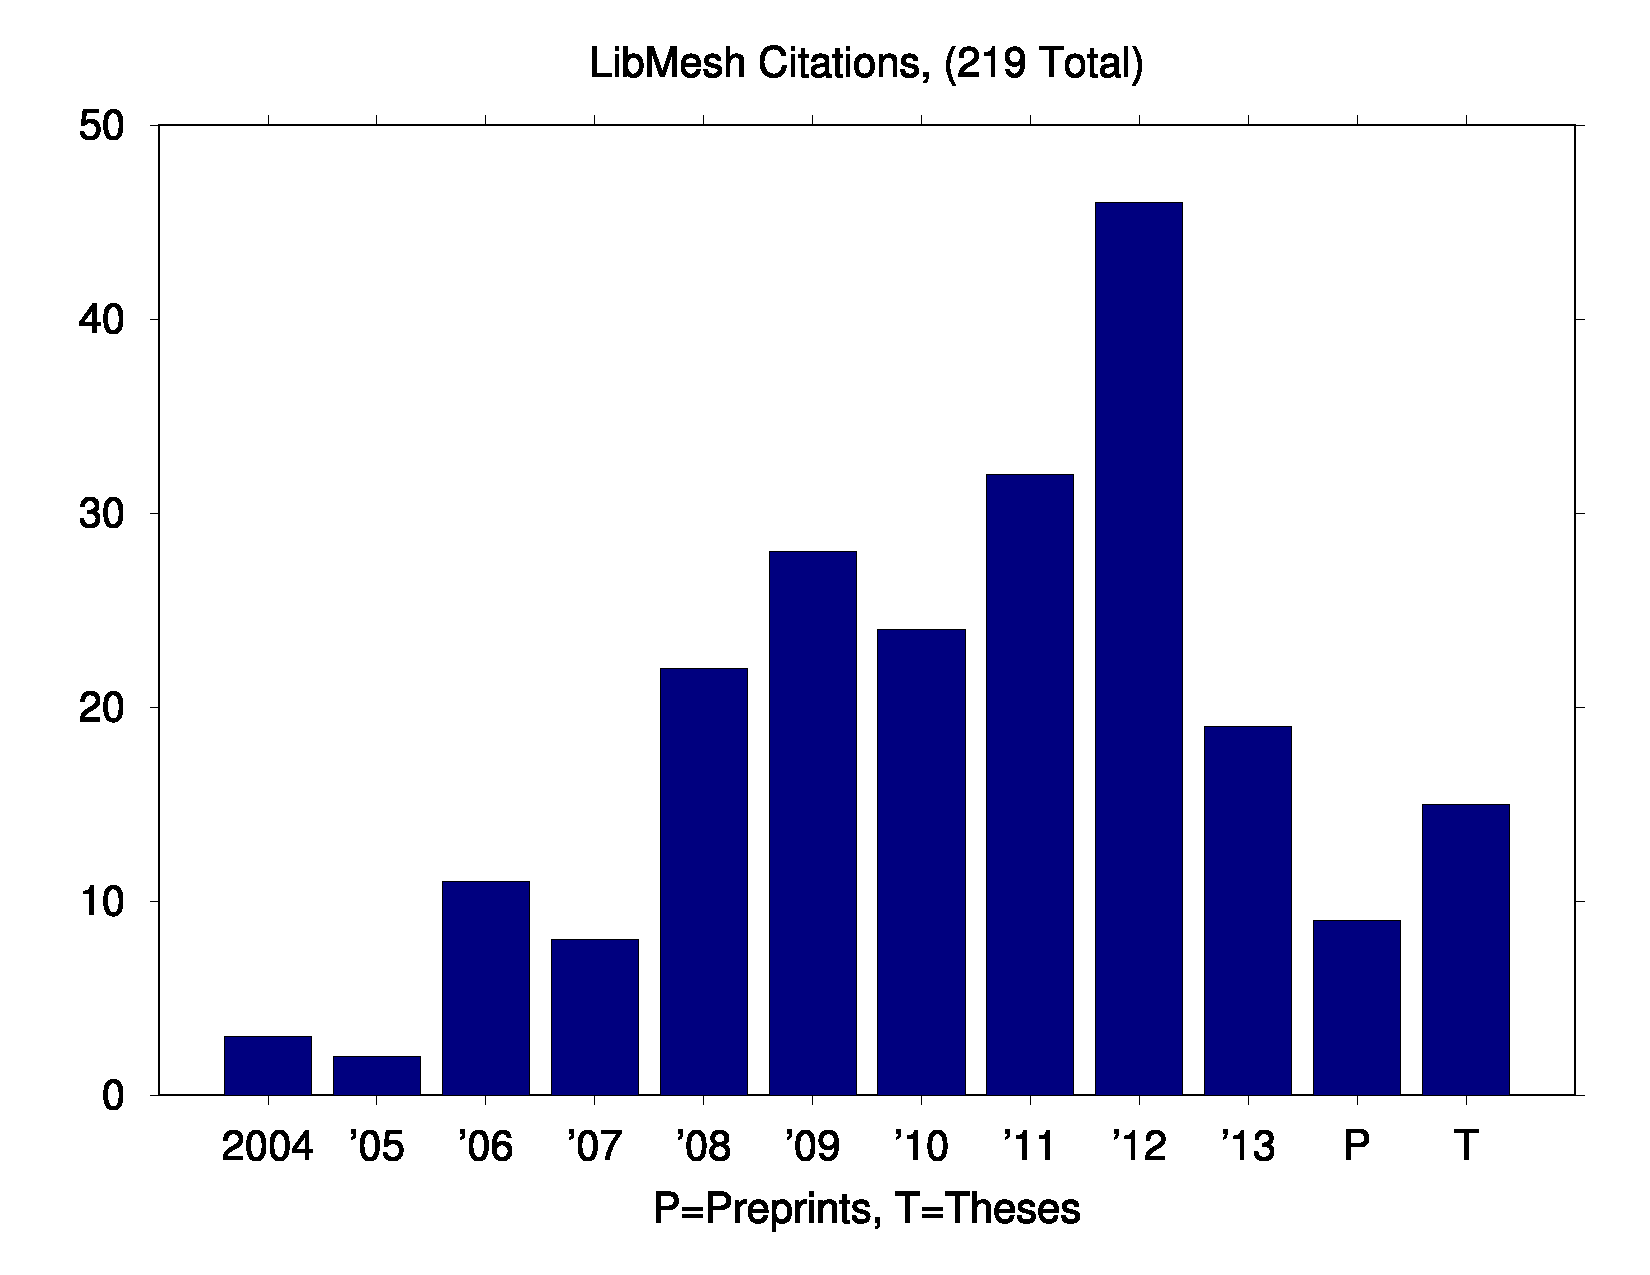
\includegraphics[height=0.8\textheight]{trivia/libmesh_citations}
  \end{center}
}       


\subsection{Library Design}
%%%%%%%%%%%%%%%%%%%%%%%%%%%%%%%%%%%%%%%%%%%%%%%%%
\frame
{
  \frametitle{The ``Glue''}
  \begin{itemize}
    \item The \cpp{} programming language provides a powerful abstraction mechanism for separating a software interface from its implementation.
    \item The notion of \emphcolor{Base Classes} defining an abstract interface and \emphcolor{Derived Classes} implementing the interface is key to this programming model.
      \pause
    \item The classic \cpp{} example: Shapes.
  \end{itemize}
  \lstinputlisting{snippets/shapes/main.cxx}
}



%%%%%%%%%%%%%%%%%%%%%%%%%%%%%%%%%%%%%%%%%%%%%%%%%
\frame
{
  \frametitle{Abstract Shape}
  \lstinputlisting{snippets/shapes/shape.cxx}
}



%%%%%%%%%%%%%%%%%%%%%%%%%%%%%%%%%%%%%%%%%%%%%%%%%
\frame
{
  \frametitle{Specific Shape: Rectangle}
  \lstinputlisting{snippets/shapes/rectangle.cxx}
}



%%%%%%%%%%%%%%%%%%%%%%%%%%%%%%%%%%%%%%%%%%%%%%%%%
\frame
{
  \frametitle{Specific Shape: Circle}
  \lstinputlisting{snippets/shapes/circle.cxx}
}



%%%%%%%%%%%%%%%%%%%%%%%%%%%%%%%%%%%%%%%%%%%%%%%%%
\frame
{
  \frametitle{Object Polymorphism}
  \lstinputlisting{snippets/shapes/main2.cxx}
}



%%%%%%%%%%%%%%%%%%%%%%%%%%%%%%%%%%%%%%%%%%%%%%%%%
\frame
{
  \Large
  \begin{block}{}
    \center{Examples of Polymorphism in}
    \center{\bf \libmesh{}}
  \end{block}
}



%%%%%%%%%%%%%%%%%%%%%%%%%%%%%%%%%%%%%%%%%%%%%%%%%
\frame
{
  \frametitle{The ``Glue:'' Linear Algebra}
  \begin{center}
    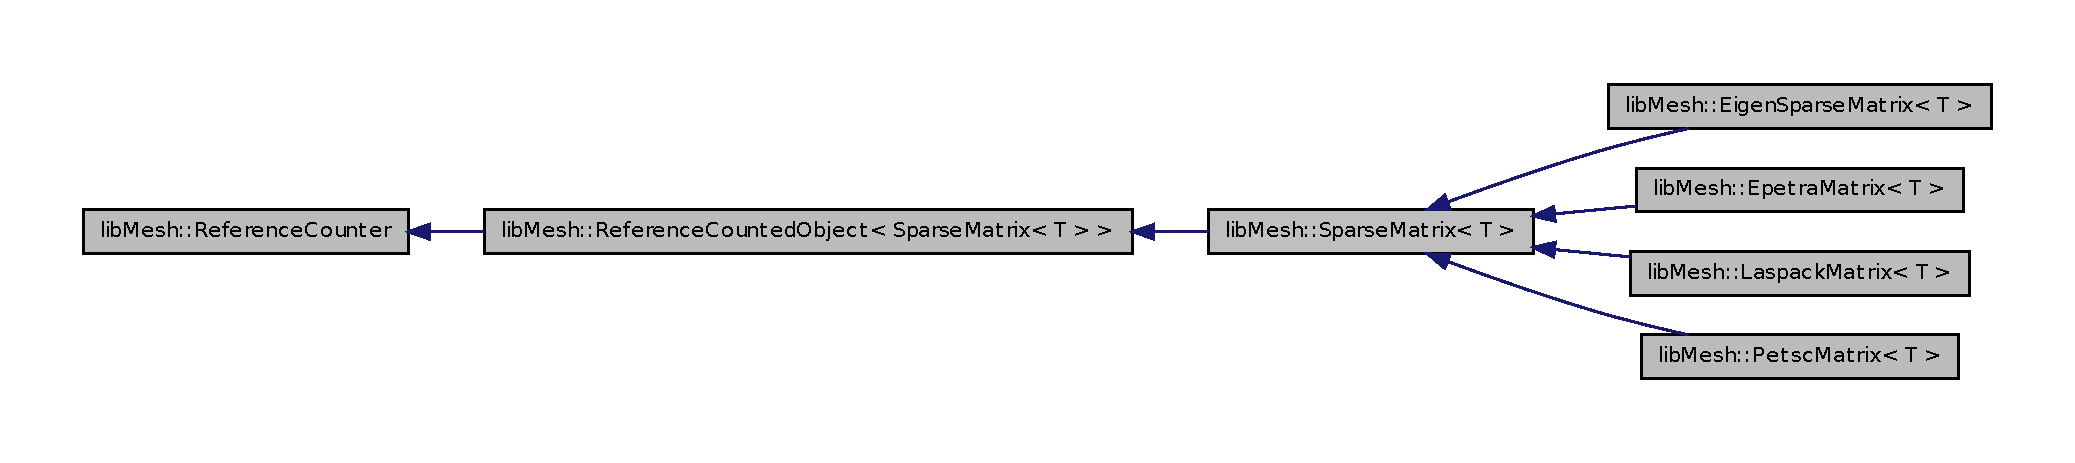
\includegraphics[width=\textwidth,trim=7.56in 0 0 0,clip]{libmesh_docs/classlibMesh_1_1SparseMatrix__inherit__graph}
  \end{center}
}



%%%%%%%%%%%%%%%%%%%%%%%%%%%%%%%%%%%%%%%%%%%%%%%%%
\frame
{
  \frametitle{The ``Glue:'' I/O formats}
  \begin{center}
    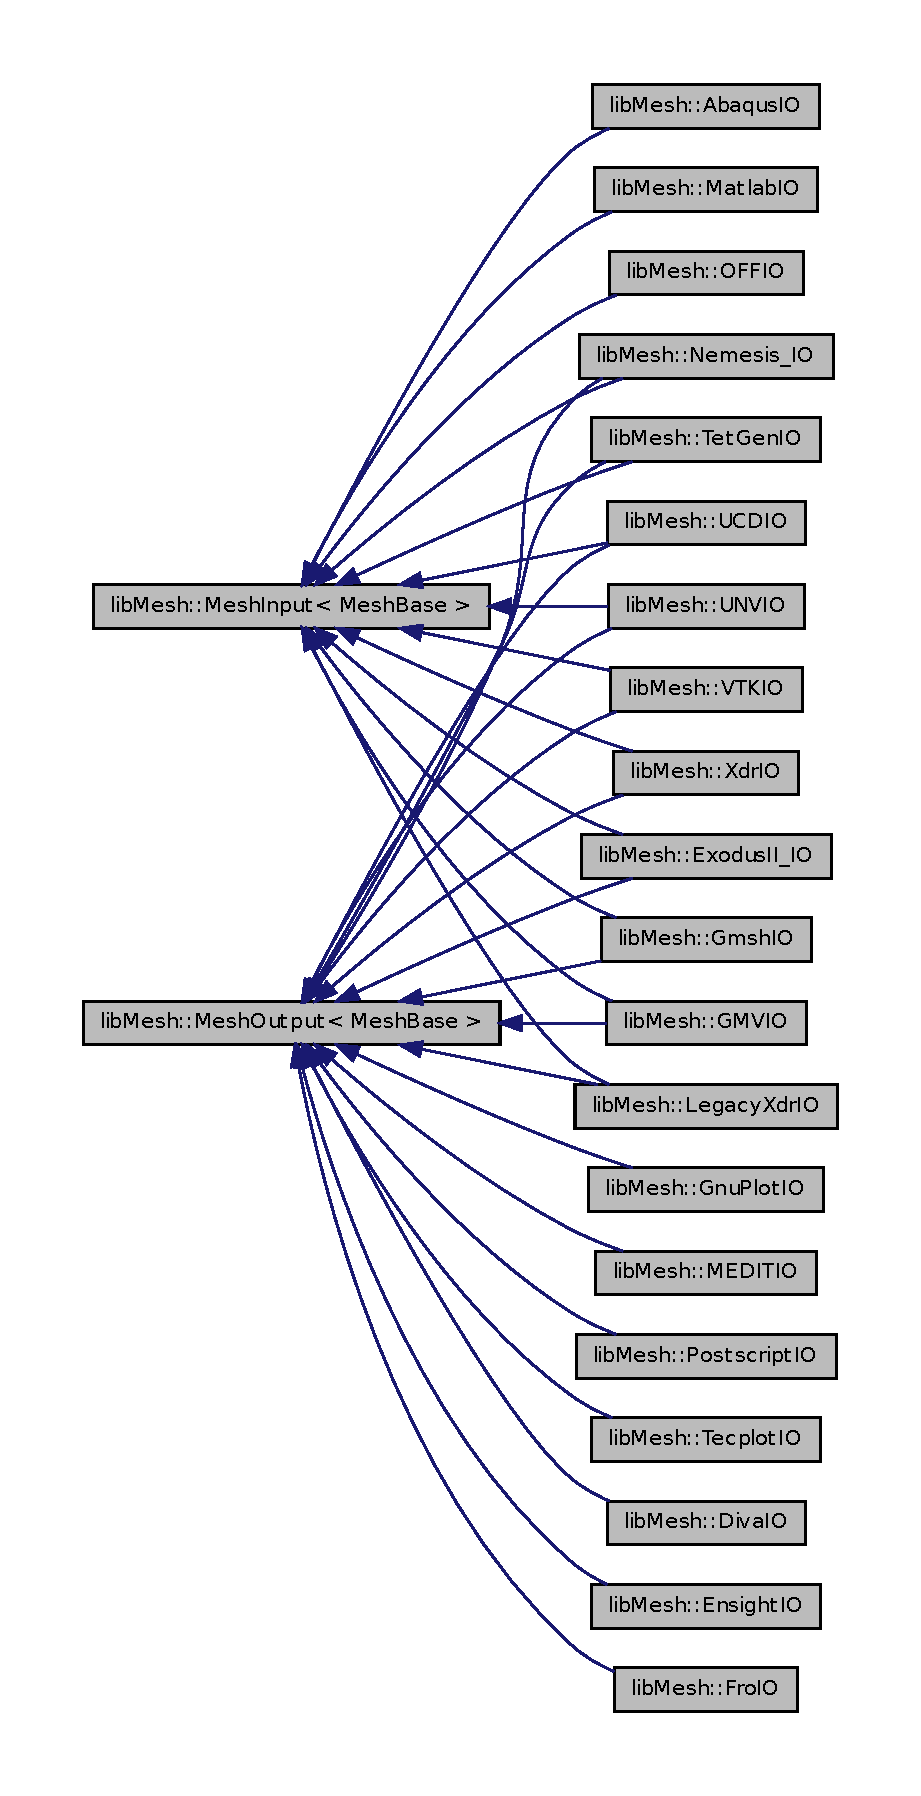
\includegraphics[height=0.9\textheight]{libmesh_docs/mesh_io}
  \end{center}
}



%%%%%%%%%%%%%%%%%%%%%%%%%%%%%%%%%%%%%%%%%%%%%%%%%
\frame
{
  \frametitle{Disretization: The Mesh}
  \begin{center}
    \includegraphics[width=\textwidth]{libmesh_docs/mesh_base}
  \end{center}
}      



%%%%%%%%%%%%%%%%%%%%%%%%%%%%%%%%%%%%%%%%%%%%%%%%%
\frame
{
  \frametitle{Disretization: Geometric Elements}
  \begin{center}
    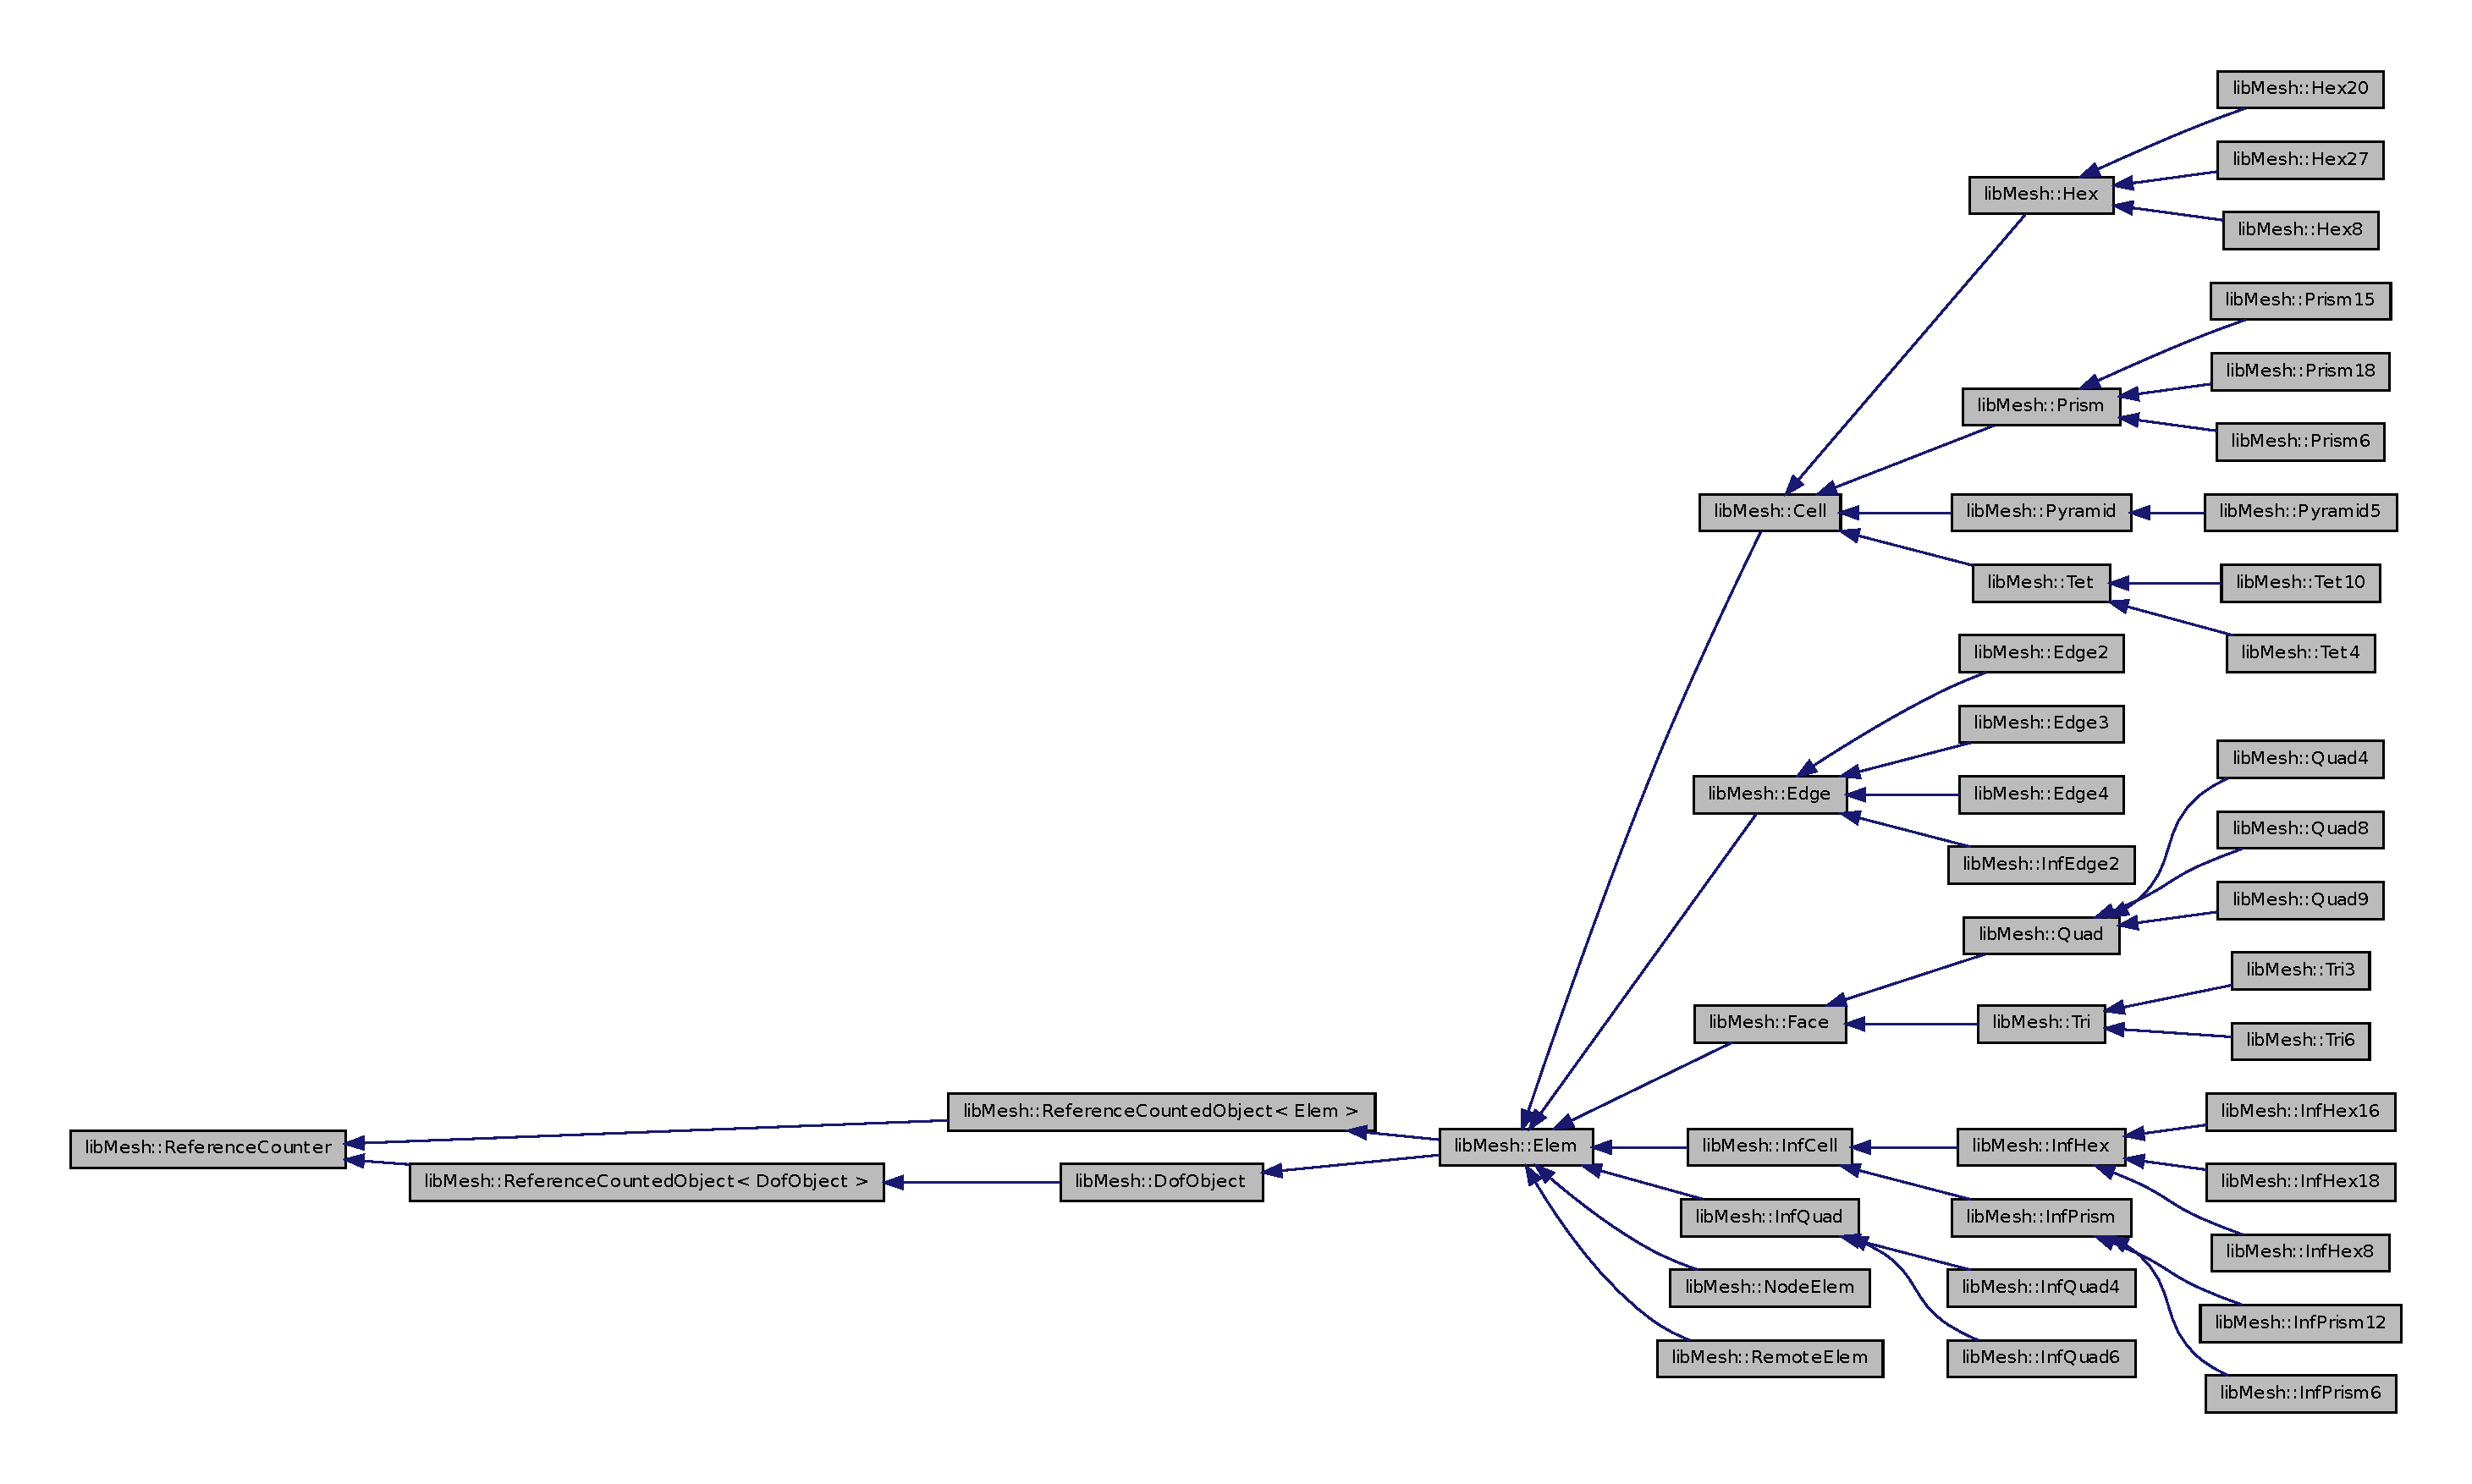
\includegraphics[width=\textwidth]{libmesh_docs/classlibMesh_1_1Elem__inherit__graph}
  \end{center}
}      



%%%%%%%%%%%%%%%%%%%%%%%%%%%%%%%%%%%%%%%%%%%%%%%%%
\frame
{
  \frametitle{Disretization: Geometric Elements}
  \begin{center}
    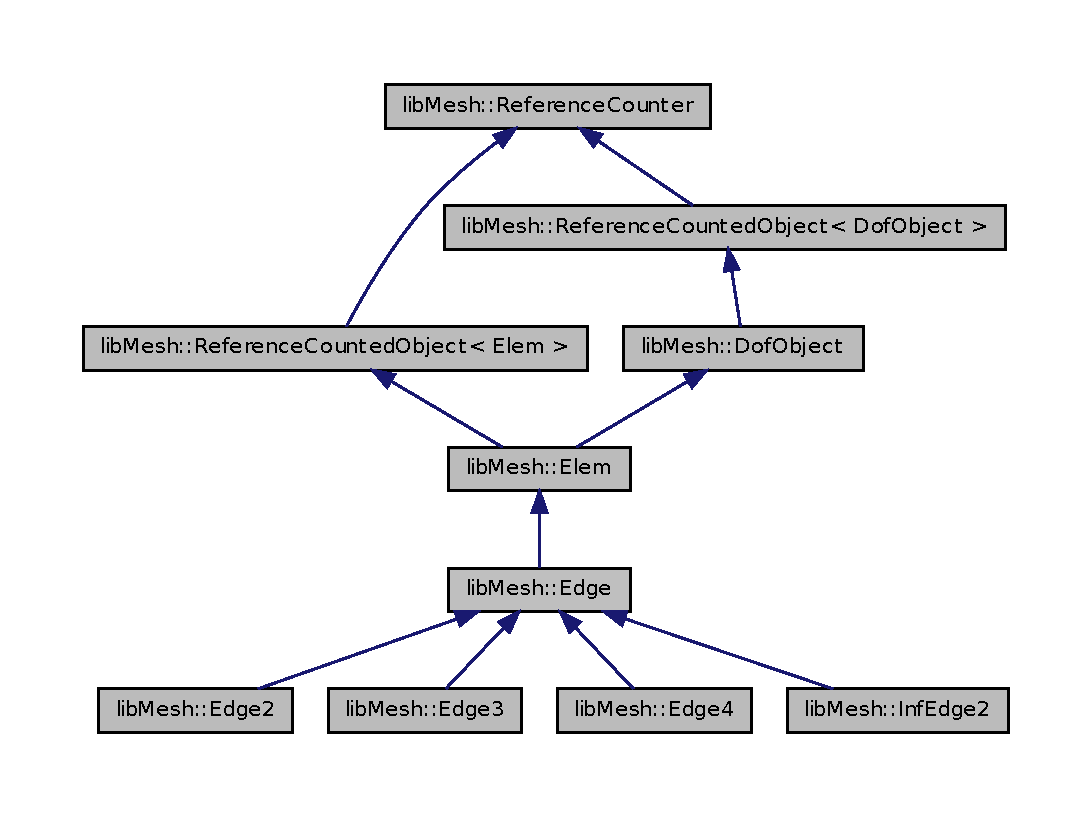
\includegraphics[width=0.9\textwidth]{libmesh_docs/classlibMesh_1_1Edge__inherit__graph}
  \end{center}
}      



%%%%%%%%%%%%%%%%%%%%%%%%%%%%%%%%%%%%%%%%%%%%%%%%%
\frame
{
  \frametitle{Disretization: Geometric Elements}
  \begin{center}
    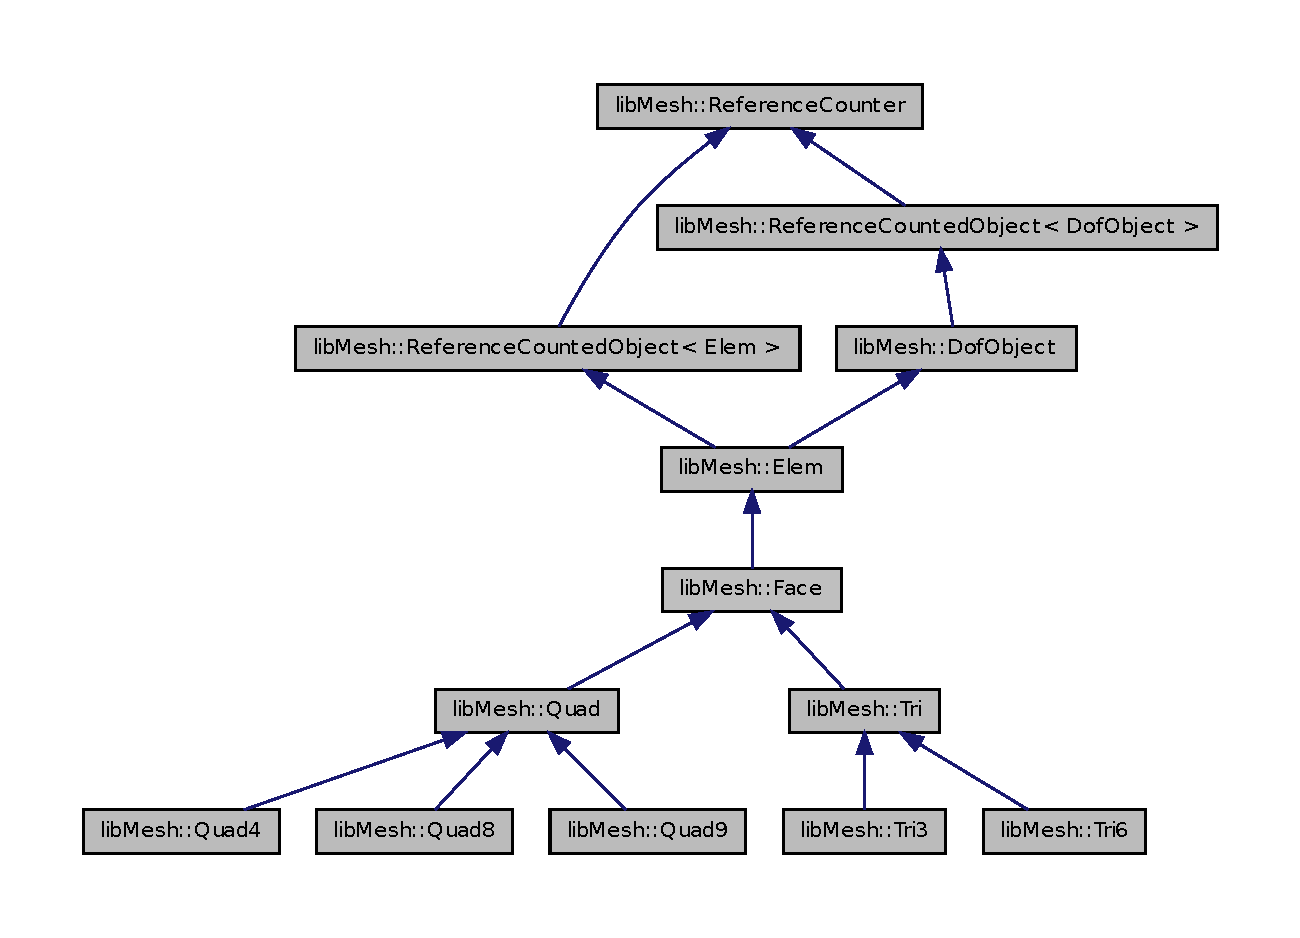
\includegraphics[width=0.95\textwidth]{libmesh_docs/classlibMesh_1_1Face__inherit__graph}
  \end{center}
}      



%%%%%%%%%%%%%%%%%%%%%%%%%%%%%%%%%%%%%%%%%%%%%%%%%
\frame
{
  \frametitle{Disretization: Geometric Elements}
  \begin{center}
    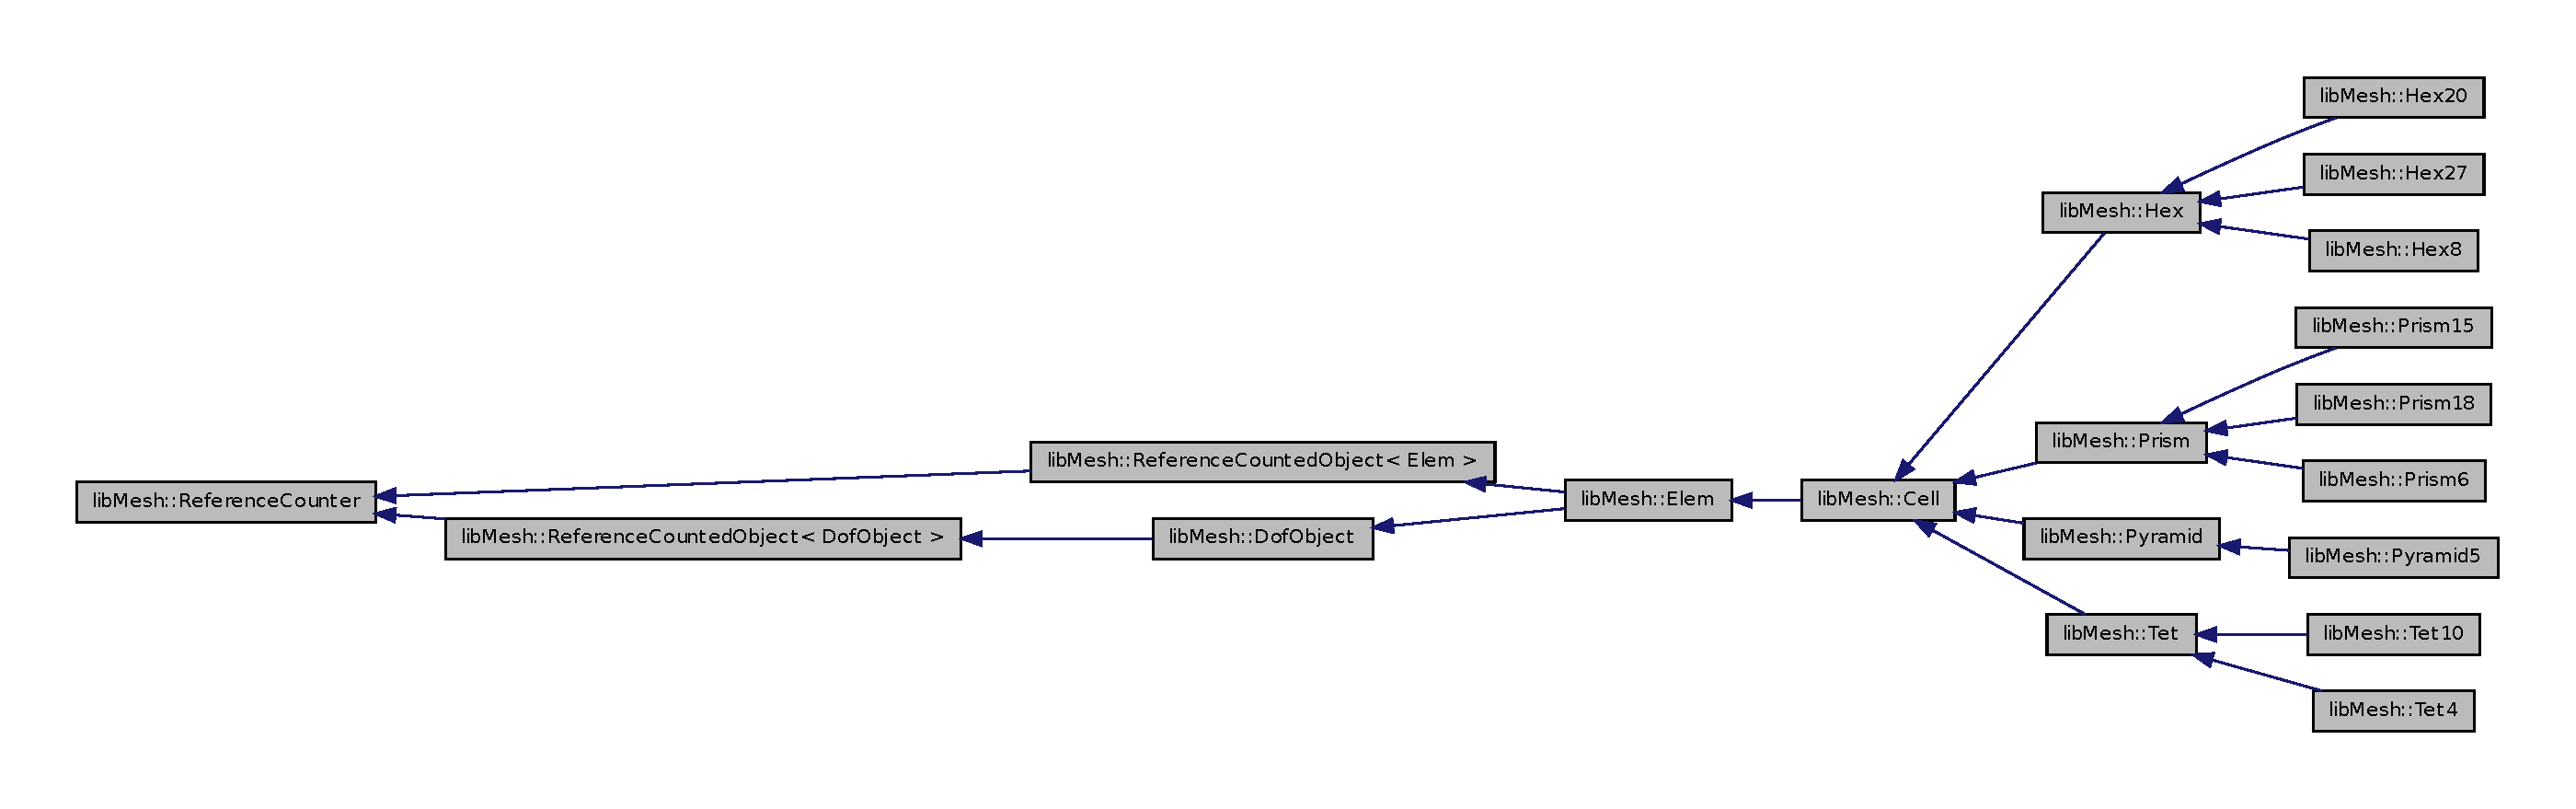
\includegraphics[width=0.9\textwidth,trim=11.3in 0 0 0,clip]{libmesh_docs/classlibMesh_1_1Cell__inherit__graph}
  \end{center}
}      



%%%%%%%%%%%%%%%%%%%%%%%%%%%%%%%%%%%%%%%%%%%%%%%%%
\frame
{
  \frametitle{Disretization: Finite Elements}
  \begin{center}
    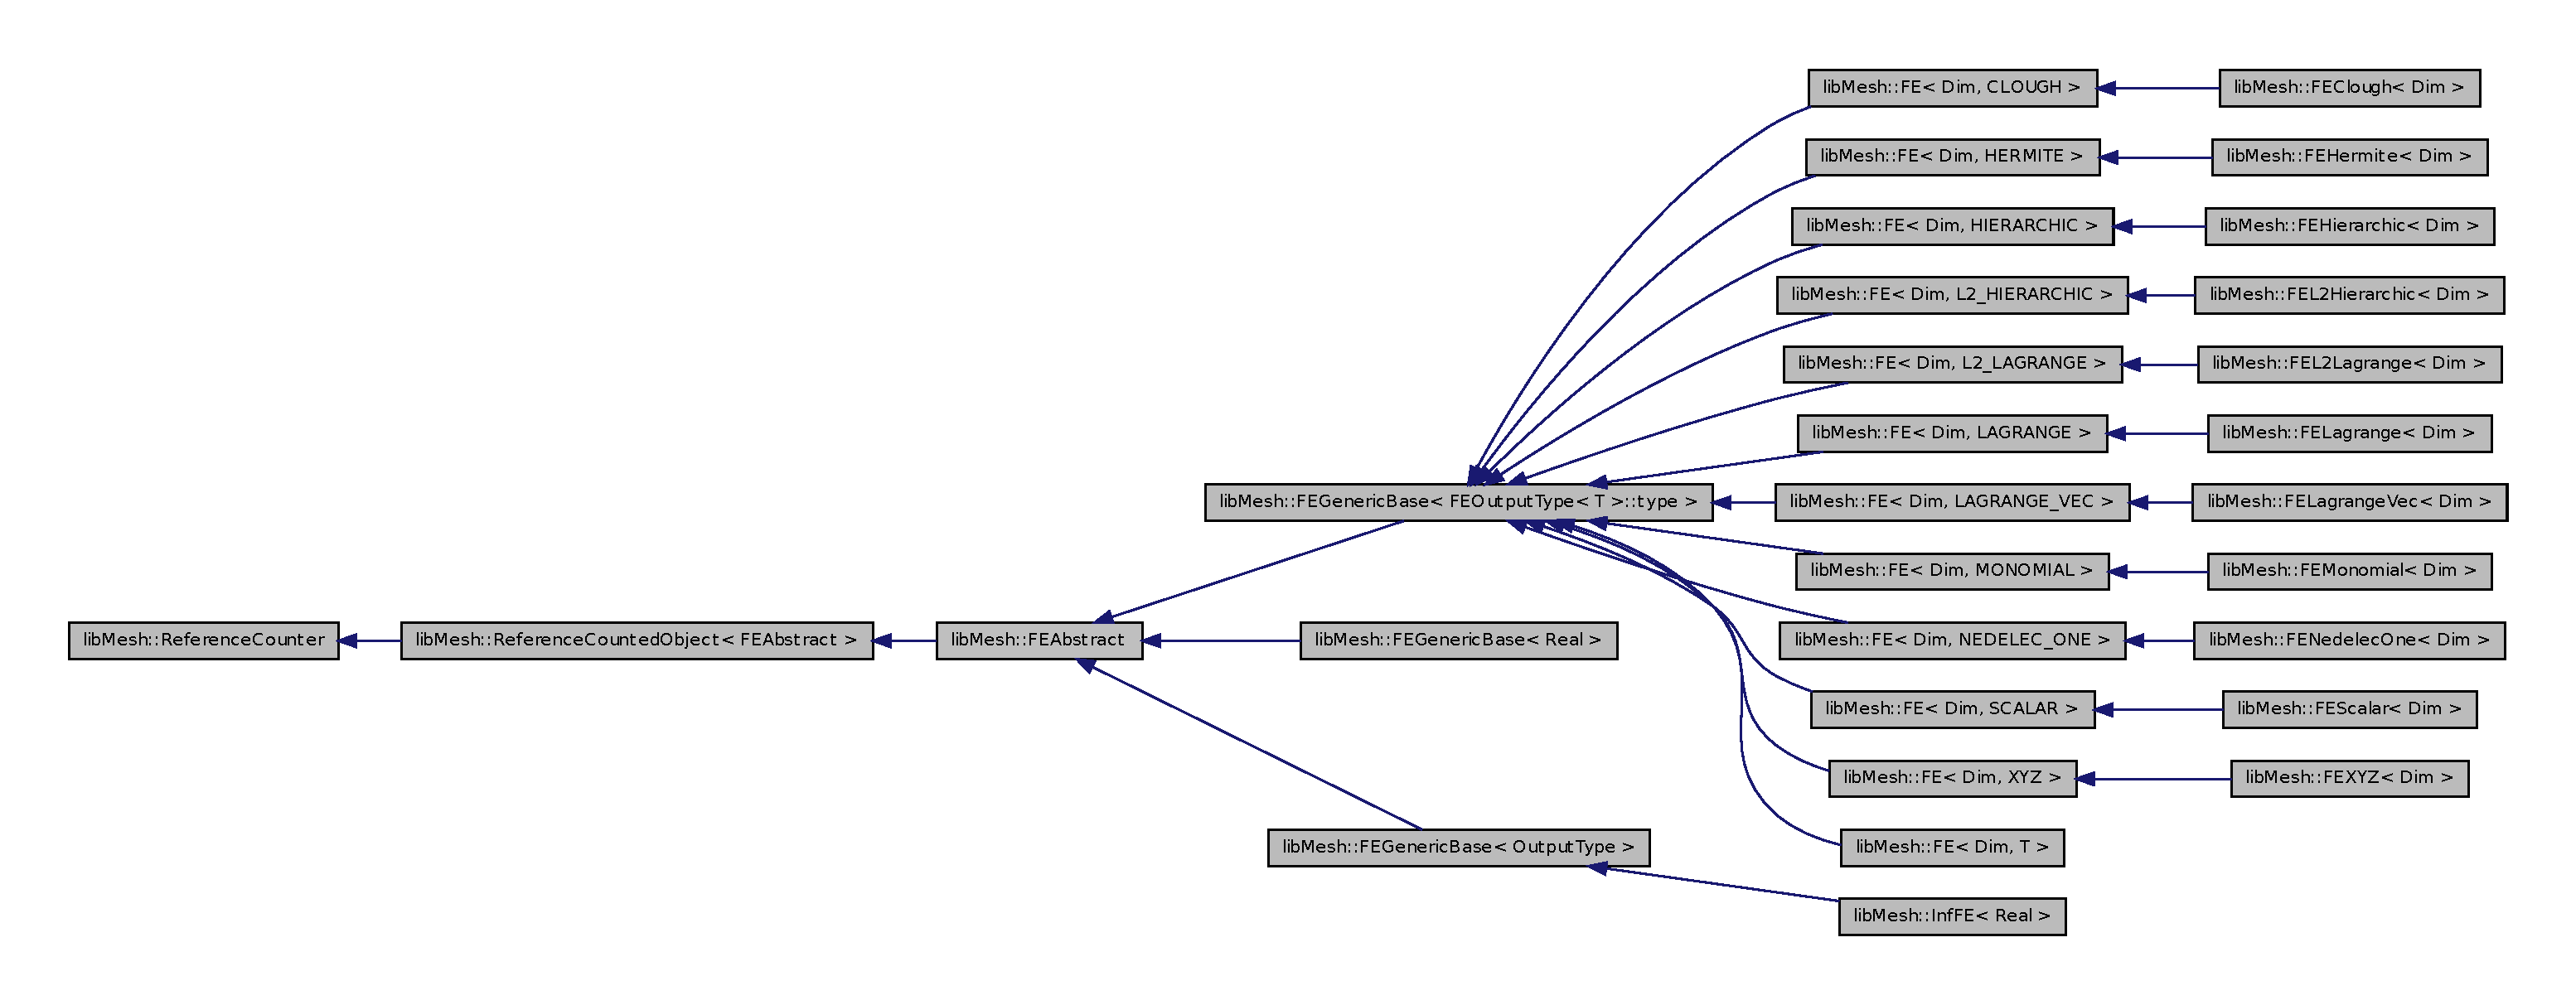
\includegraphics[width=0.9\textwidth,trim=7.4in 0 0 0,clip]{libmesh_docs/classlibMesh_1_1FEAbstract__inherit__graph}
  \end{center}
}      



%%%%%%%%%%%%%%%%%%%%%%%%%%%%%%%%%%%%%%%%%%%%%%%%%
\frame
{
  \frametitle{Algorithms: Domain Partitioning}
  \begin{center}
    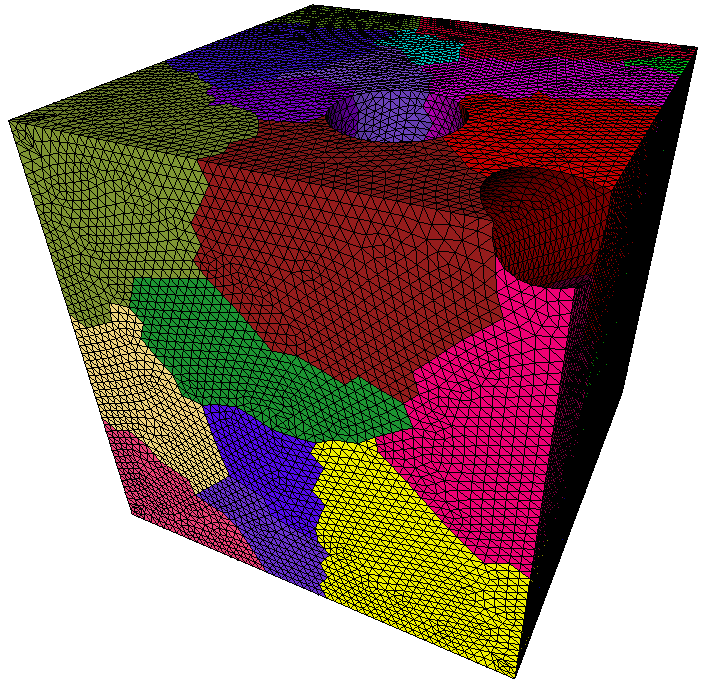
\includegraphics[width=.45\textwidth]{part_trans}
    %\\
    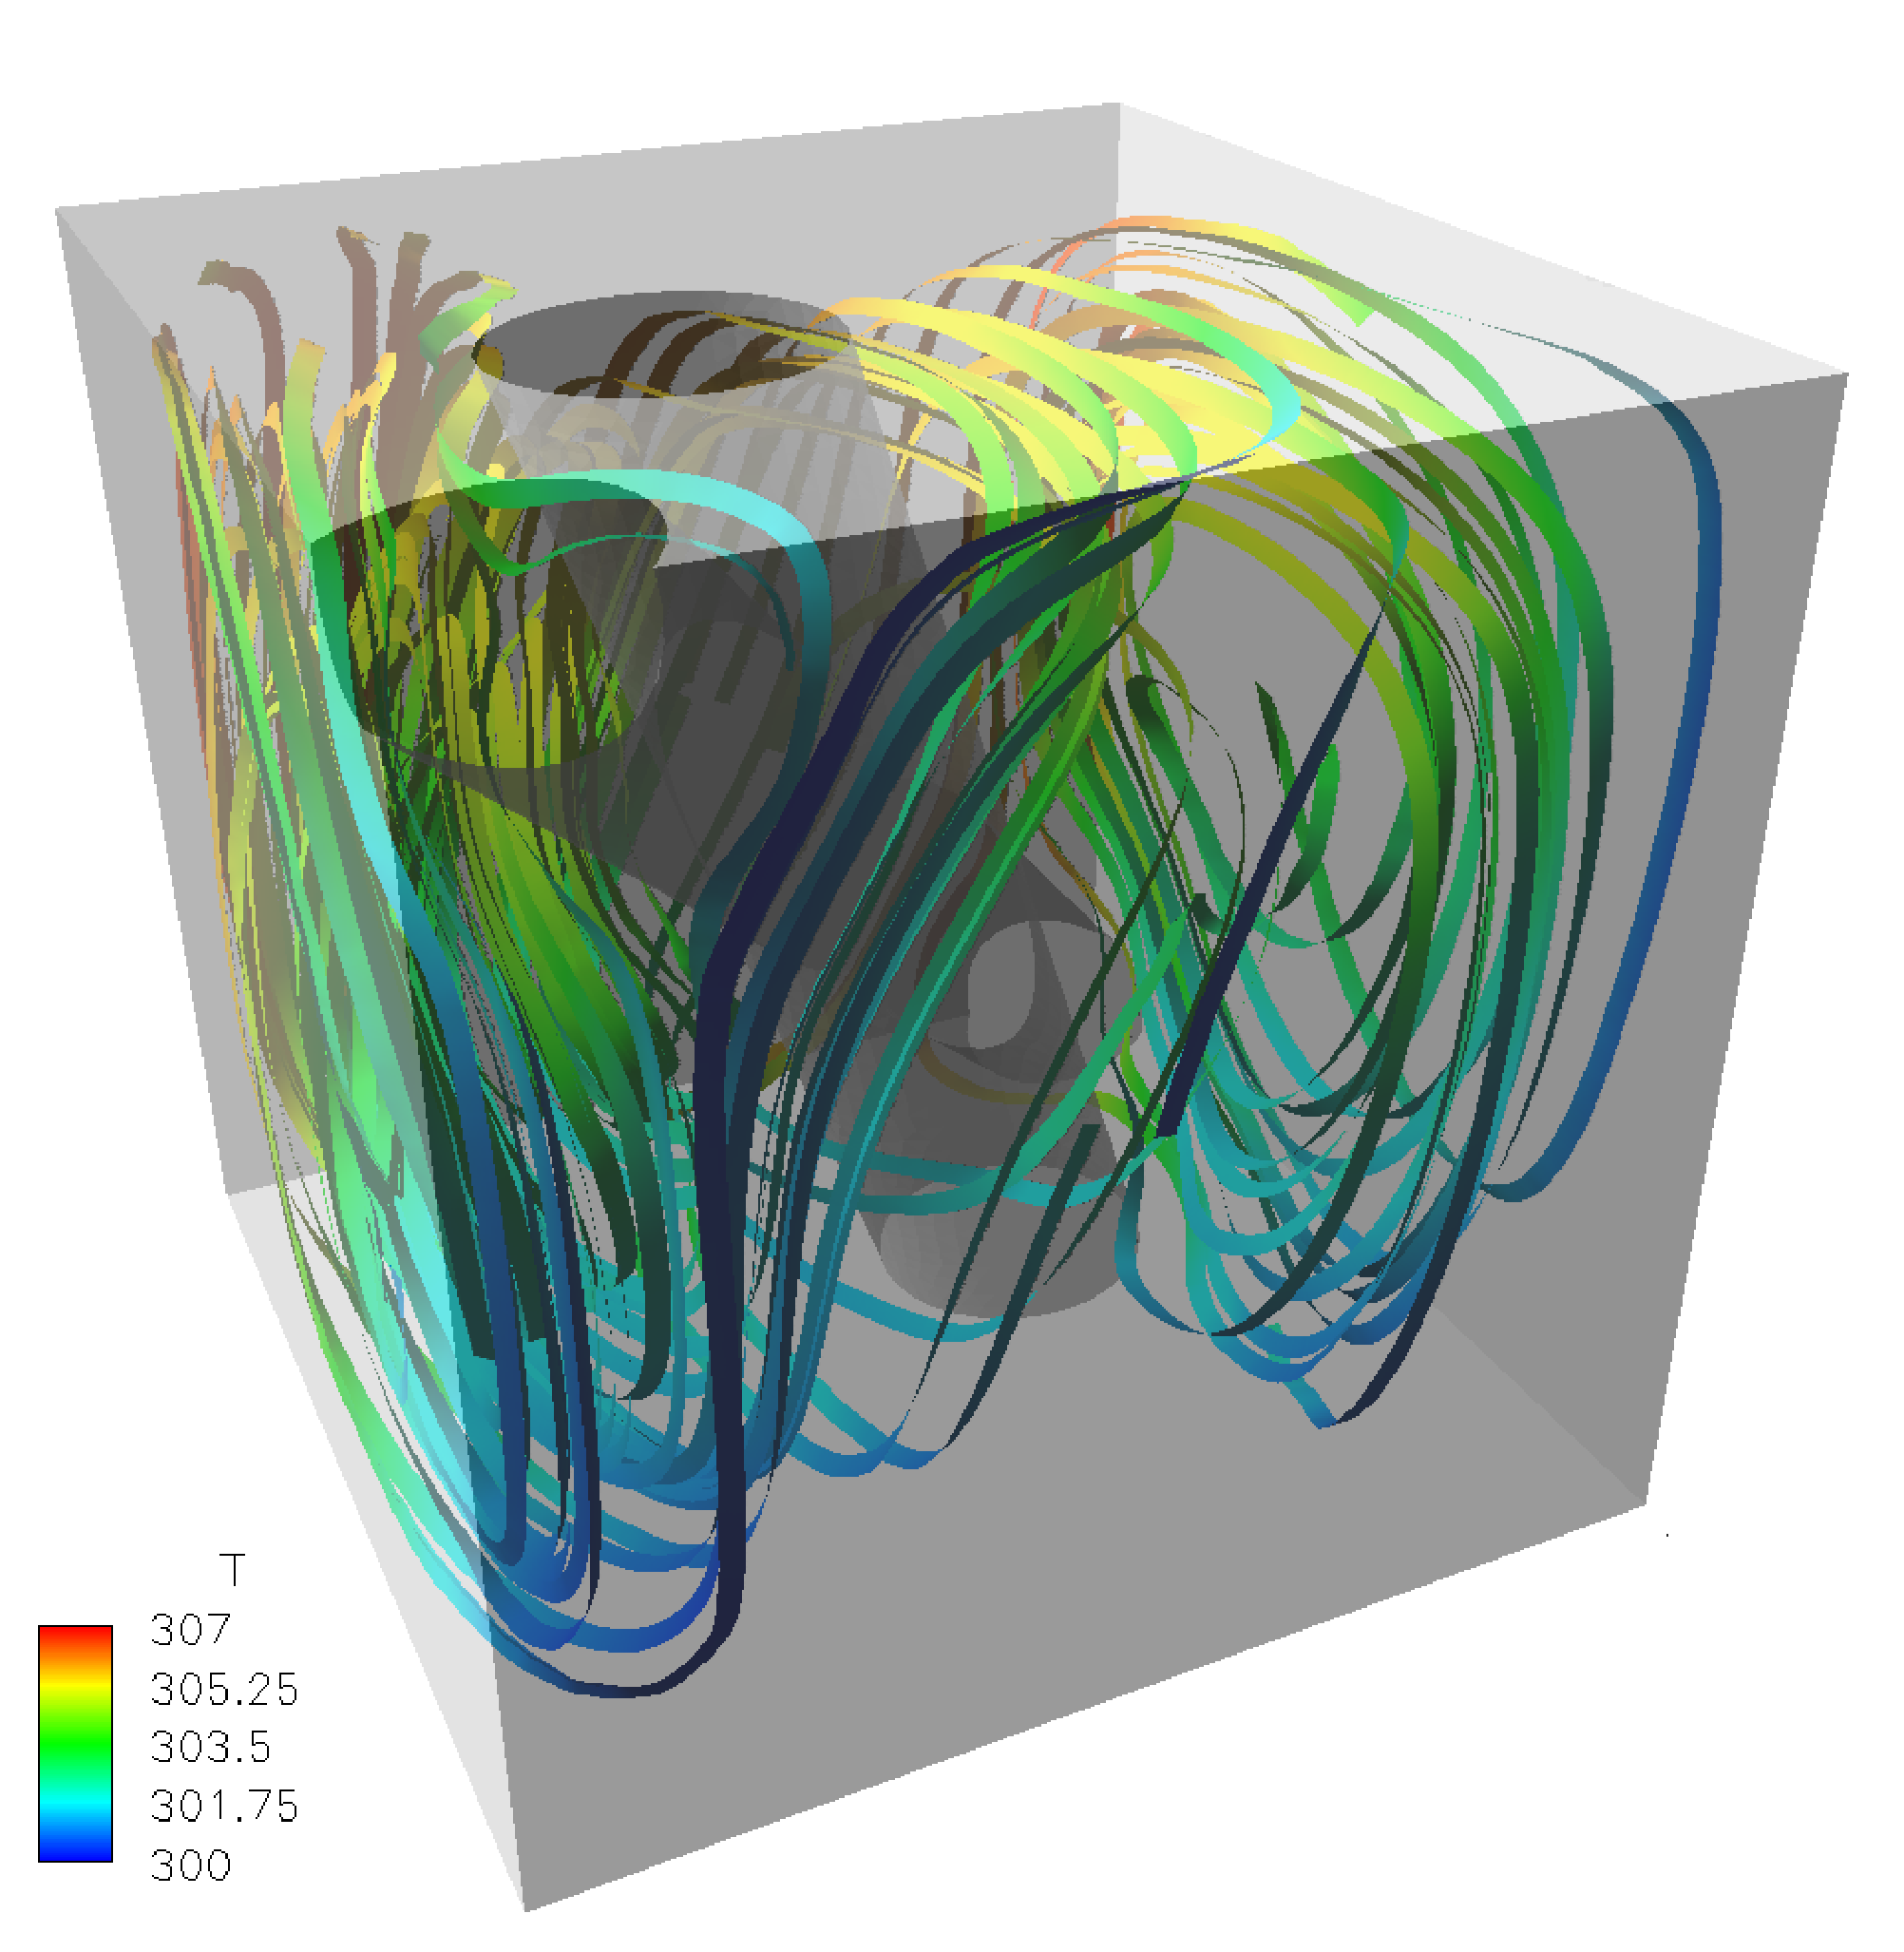
\includegraphics[width=.45\textwidth]{streamtraces}
  \end{center}  
}



%%%%%%%%%%%%%%%%%%%%%%%%%%%%%%%%%%%%%%%%%%%%%%%%%
\frame
{
  \frametitle{Algorithms: Domain Partitioning}
  \begin{center}
    \includegraphics[width=\textwidth]{libmesh_docs/partitioner}
  \end{center}
}


%%%%%%%%%%%%%%%%%%%%%%%%%%%%%%%%%%%%%%%%%%%%%%%%%
\frame
{
  \frametitle{Algorithms: Error Estimation}
  \begin{center}
    \includegraphics[width=\textwidth]{libmesh_docs/error_estimation}
  \end{center}
}





% LocalWords:  nasablue

% The optional argument [<+->] means everything on the frame will be displayed incrementally.
\section{Introduction}

\begin{frame}[<+->]
  \frametitle{Goals}   
  \begin{block}{\texttt{libMesh} is not}
  \begin{itemize}
  \item {A physics implementation.}
  \item {A stand-alone application.}
  \end{itemize}
  \end{block}
  \begin{block}{\texttt{libMesh} is}
  \begin{itemize}
  \item {A software library and toolkit.}
  \item {Classes and functions for writing parallel adaptive finite
element applications.}
  \item {An interface to linear algebra, meshing, partitioning, etc.
libraries.}
  \end{itemize}
  \end{block}
\end{frame}


\begin{frame}
  %\frametitle{}
  \begin{columns}[t]
    \column{.5\textwidth}
    \begin{block}{}%A general class of PDE}      %find $u(\bv{x},t)$ such that
      For most applications we assume there is a Boundary Value Problem
      to be approximated in a Finite Element function space
      \begin{eqnarray}
	\label{eqn:general_pde}
	\nonumber
	M \dt{u} & = & F( u ) \;\;\;\; \in \Omega
        \\
	\nonumber
	G( u ) & = & 0 \;\;\;\; \in \Omega
	\\
	\nonumber
	u & = & u_D \;\; \in \partial \Omega_D
	\\
	\nonumber
	N(u) & = & 0 \;\; \in \partial \Omega_N
 	\\
 	\nonumber
 	u(\bv{x}, 0) & = & u_0(\bv{x}) 
      \end{eqnarray}
    \end{block}
    %\pause
    \column{.5\textwidth}
    %\begin{block}{}
      \begin{center}
	%\fbox{
	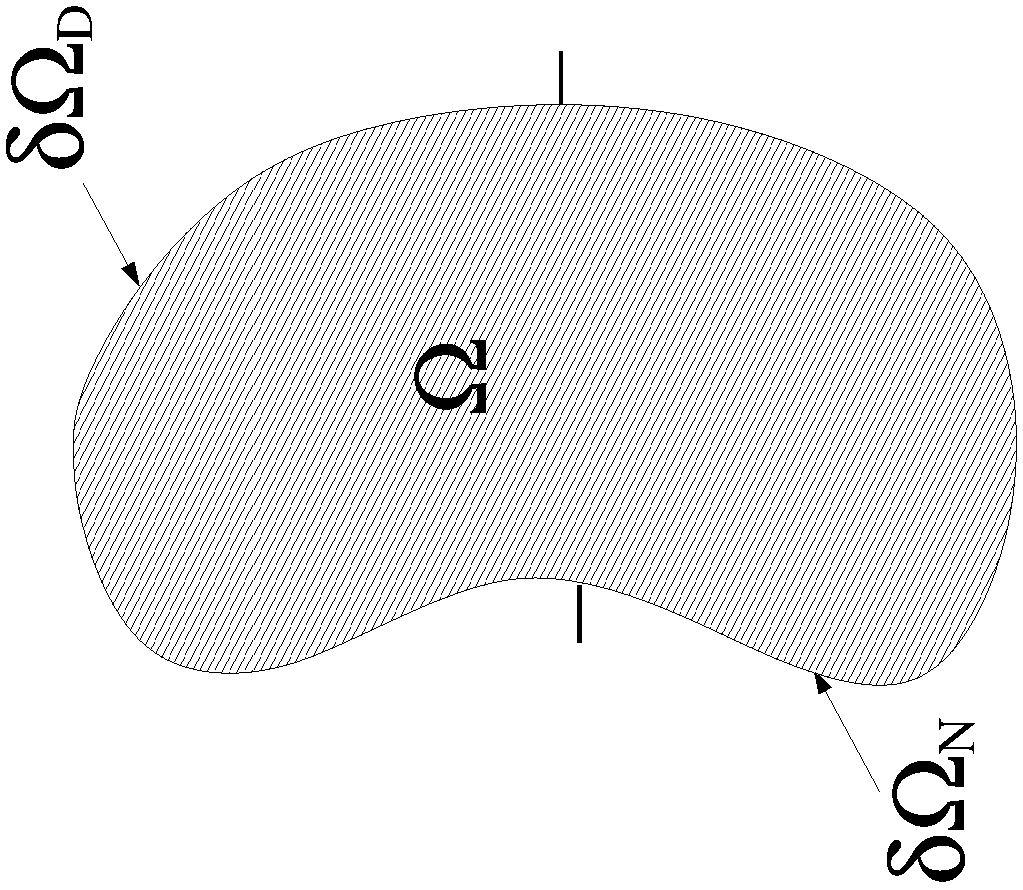
\includegraphics[width=2in,angle=-90]{figs/domain}
	%}
      \end{center}
    %\end{block}
  \end{columns}
%%  \begin{itemize}
%%    \item $\mathcal{N}( u )$ is a nonlinear operator which depends on the unknown
%%      $u$ and its spatial gradients%, $\bv{f}$ is a forcing function
%%    % \item With slight modifications, a wide range of physically interesting problems fall into this class
%%    \item Use generic numerical methods to treat many problems in the same framework
%%  \end{itemize}
\end{frame}


\begin{frame}
  %\frametitle{}
  \begin{columns}[t]
    \column{.5\textwidth}
    \begin{block}{}%A general class of PDE}
      \begin{itemize}
      \item{
	Associated to $\Omega$ is the \texttt{Mesh} data
	structure
      }
	
      \item{A \texttt{Mesh} is basically
	a collection of geometric elements and nodes}
      \end{itemize}
      \begin{equation}
	\label{eqn:discretized_domain}
	\nonumber
	\Omega^h:=\bigcup_e \Omega_e
      \end{equation}
    \end{block}
    %\pause
    \column{.5\textwidth}
    %\begin{block}{}
      \begin{center}
	%\fbox{
	\includegraphics[width=2in,angle=-90]{figs/discretized_domain}
	%}
      \end{center}
    %\end{block}
  \end{columns}
\commentout{
  \visible<2>
  {
  \begin{itemize}
    \item{libMesh provides some simple structured mesh generation routines
      as well as an interface to Triangle.}
  \end{itemize}
  }
}
\end{frame}


%% \begin{frame}
%%   \frametitle{The Mesh}
%%   \begin{block}{}
%%     The \texttt{Mesh} data structure provides: 
%%     \begin{itemize}
%%     \item{Iterator access to the nodes and elements}
%%     \end{itemize}
%%   \end{block}
%% \end{frame}


\section{Object Models}
      
\begin{frame}[<+->]
\frametitle{Object Oriented Programming}

  \royitemizebegin{OOP Fundamentals}
    \item Abstract Base Classes define user interfaces
    \item Concrete Subclasses implement functionality
    \item Interface user can choose any implementation
  \royitemizeend
\end{frame}

\subsection{Core Classes}

%%%%%%%%%%%%%%%%%%%%%%%%%%%%%%%%%%%%%%%%%%%%%%%%%%%%%%%%%%%%%%%%%%%%%
\begin{frame}
\frametitle{Geometric Element Classes}

\begin{minipage}[h]{.45\textwidth}
\begin{center}
\includegraphics[width=.9\textwidth]{figs/DofObjects}
\end{center}
\end{minipage}
\begin{minipage}[h]{.45\textwidth}
\royitemizebegin{}
\item Abstract interface gives mesh topology
\item Concrete instantiations of mesh geometry
\item Hides element type from most applications
\royitemizeend
\end{minipage}

\end{frame}

%%%%%%%%%%%%%%%%%%%%%%%%%%%%%%%%%%%%%%%%%%%%%%%%%%%%%%%%%%%%%%%%%%%%%
\begin{frame}
\frametitle{Finite Element Classes}

\begin{minipage}[h]{.45\textwidth}
\begin{center}
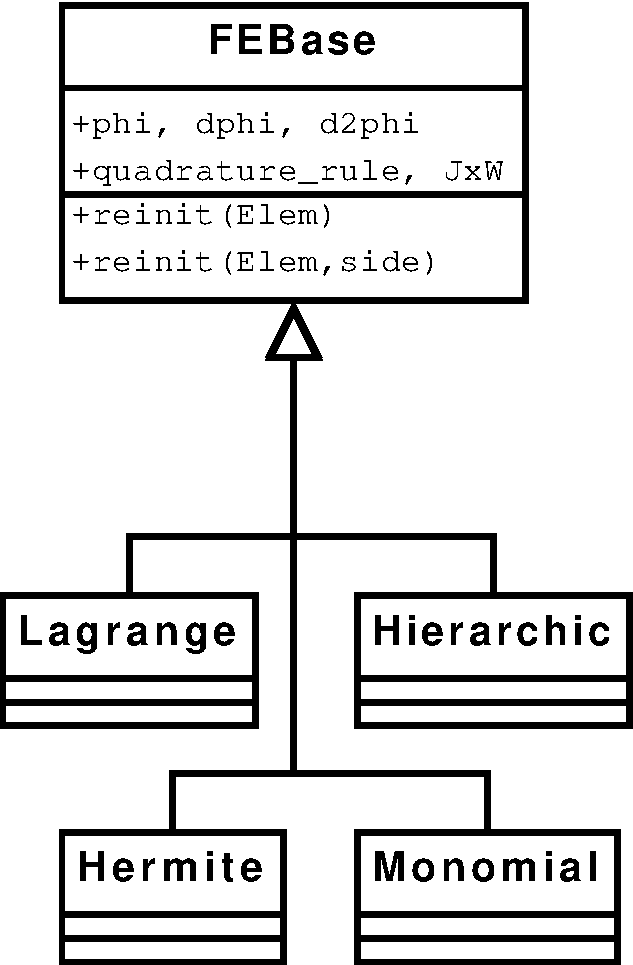
\includegraphics[width=.9\textwidth]{figs/FE}
\end{center}
\end{minipage}
\begin{minipage}[h]{.45\textwidth}
\royitemizebegin{}
\item Finite Element object builds data for each geometric Elem object
\item User only deals with shape function, quadrature data
\royitemizeend
\end{minipage}

\end{frame}

%%%%%%%%%%%%%%%%%%%%%%%%%%%%%%%%%%%%%%%%%%%%%%%%%%%%%%%%%%%%%%%%%%%%%
\begin{frame}
\frametitle{Quadrature Rule Classes}

\begin{minipage}[h]{.45\textwidth}
\begin{center}
\includegraphics[width=.9\textwidth]{figs/Quadrature}
\end{center}
\end{minipage}
\begin{minipage}[h]{.45\textwidth}
\royitemizebegin{}
\item Takes p refinement level from FE, geometric Elem objects
\item Builds requested quadrature rule for FE object
\item Caching for repeated use
\royitemizeend
\end{minipage}

\end{frame}

\commentout{
%%%%%%%%%%%%%%%%%%%%%%%%%%%%%%%%%%%%%%%%%%%%%%%%%%%%%%%%%%%%%%%%%%%%%
\begin{frame}
\frametitle{Core Features}

\royitemizebegin{}
\item Mixed element geometries in unstructured grids
\item Adaptive mesh h refinement with hanging nodes, p refinement
\item Integration w/ PETSc, LASPack, METIS, ParMETIS, Triangle, TetGen
\item Support for UNV, ExodusII, Tecplot, GMV, UCD files
\item Mesh creation, modification utilities
\royitemizeend

\end{frame}
}

      
\begin{frame}[<+->]
\frametitle{Degree of Freedom Handling}

  \begin{block}{}
  \begin{itemize}
    \item{DofObject subclasses store global Degree of Freedom indices}
    \item{DofMap class assigns indices to a partitioned mesh}
    \item{FE classes calculate hanging node, periodic constraints}
    \item{DofMap class applies constraints}
    \item{System class handles AMR/C projections}
  \end{itemize}
  \end{block}
\end{frame}


\begin{frame}
\frametitle{Generic Constraint Calculations}

To maintain function space continuity, constrain ``hanging node''
Degrees of Freedom coefficients on fine elements in terms of DoFs on
coarse neighbors.

\begin{minipage}[h]{.45\textwidth}
  \begin{figure}[h]
    \begin{center}
      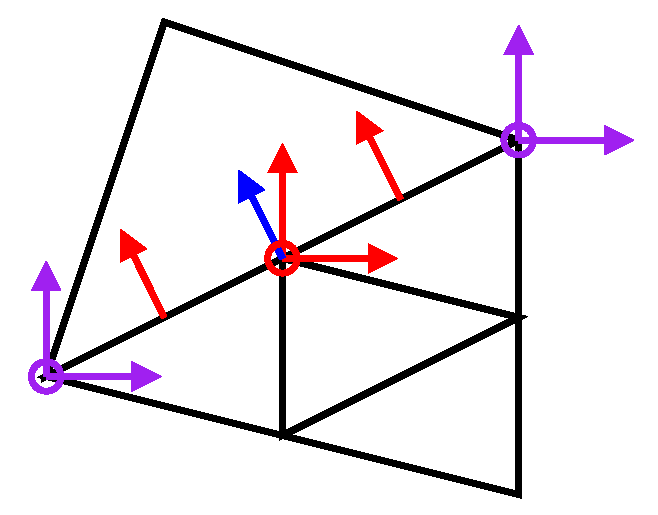
\includegraphics[width=.5\textwidth]{figs/hanging_node}
    \end{center}
  \end{figure}
\end{minipage}
\begin{minipage}[h]{.45\textwidth}
\begin{eqnarray*}
u^F & = & u^C \\
\sum_i u_i^F \phi_i^F & = & \sum_j u_j^C \phi_j^C \\
A_{ki} u_i & = & B_{kj} u_j \\
u_i & = & A_{ki}^{-1} B_{kj} u_j
\end{eqnarray*}
\end{minipage}

Integrated values (and fluxes, for $C^1$ continuity) give
element-independent matrices:
\begin{eqnarray*}
A_{ki} & \equiv & (\phi_i^F, \phi_k^F) \\
B_{kj} & \equiv & (\phi_j^C, \phi_k^F)
\end{eqnarray*}

\end{frame}



\begin{frame}
\frametitle{Generic Projection Calculations}

Upon element coarsening (or refinement in non-nested spaces):

  \begin{block}{}
  \begin{itemize}
    \item{Copy nodal Degree of Freedom coefficients}
    \item{Project edge DoFs, holding nodal DoFs constant}
    \item{Project face DoFs, holding nodes/edges constant}
    \item{Project interior DoFs, holding boundaries constant}
  \end{itemize}
  \end{block}

  \begin{block}{Advantages / Disadvantages}
  \begin{itemize}
    \item{Requires only local solves}
    \item{Consistent in parallel}
    \item{May violate physical conservation laws}
  \end{itemize}
  \end{block}

\end{frame}

      
\begin{frame}[<+->]
\frametitle{libMesh Parallelization}

  \begin{block}{Parallel code}
  \begin{itemize}
    \item{PetscVector, DistributedVector classes for Linear Algebra}
    \item{Parallel assembly, error indicators, etc.}
    \item{Mesh partitioning with ParMETIS, etc.}
  \end{itemize}
  \end{block}

  \begin{block}{Serial code}
  \begin{itemize}
    \item{Mesh storage on every node}
    \item{DoF renumbering, constraint calculations}
    \item{Refinement/Coarsening flagging}
    \item{Mesh, solution I/O}
  \end{itemize}
  \end{block}
\end{frame}


\begin{frame}
\frametitle{ParallelMesh}

  \begin{block}{Parallel subclassing of MeshBase}
  \begin{itemize}
    \item{Start from unstructured Mesh class}
    \item{Add methods to delete, reconstruct non-semilocal Elem and Node objects}
    \item{Parallelize DofMap methods}
    \item{Parallelize MeshRefinement methods}
    \item{Add parallel or chunked I/O support}
    \item{Add load balancing support}
  \end{itemize}
  \end{block}

Also want parallel BoundaryInfo, BoundaryMesh, Data, Function, Generation,
Modification, Smoother, and Tools classes

\end{frame}

\subsection{Boundary Value Problem Classes}

%%%%%%%%%%%%%%%%%%%%%%%%%%%%%%%%%%%%%%%%%%%%%%%%%%%%%%%%%%%%%%%%%%%%%
\royslide{Boundary Value Problem Classes}{
\royitemizebegin{Goals}
\item Improved test coverage and reliability
\item Hiding implementation details from user code
\item Rapid prototyping of new formulations
\item Physics-dependent error estimators
\royitemizeend

\royitemizebegin{Methods}
\item Object-oriented System and Solver subclasses
\item Factoring common patterns into library code
\item Per-element Numerical Jacobian verification
\royitemizeend
}

%%%%%%%%%%%%%%%%%%%%%%%%%%%%%%%%%%%%%%%%%%%%%%%%%%%%%%%%%%%%%%%%%%%%%
\royslide{FEM System Classes}{

\begin{minipage}[h]{.45\textwidth}
\begin{center}
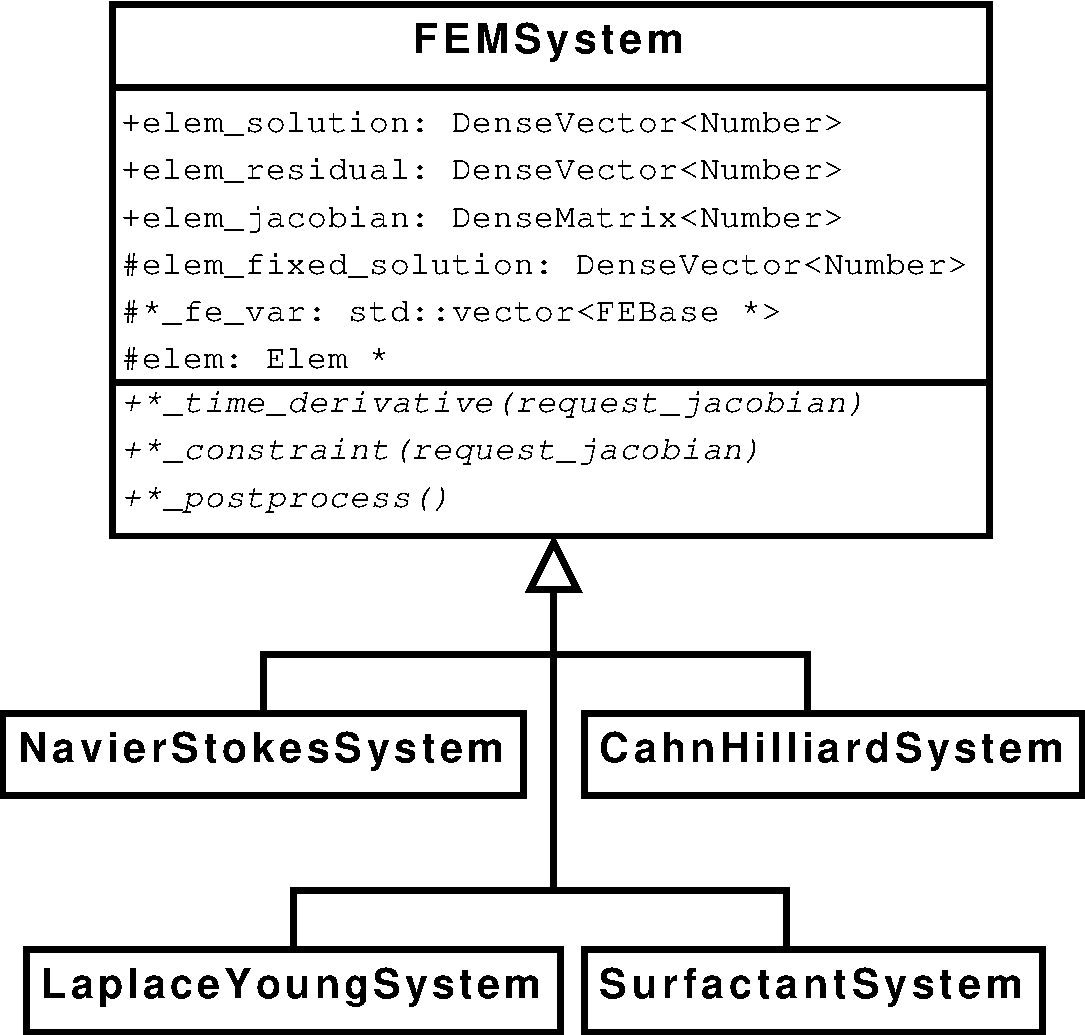
\includegraphics[width=.9\textwidth]{figs/FEMSystem}
\end{center}
\end{minipage}
\begin{minipage}[h]{.45\textwidth}
\royitemizebegin{}
\item Generalized IBVP representation
\item FEMSystem does all initialization, global assembly
\item User code only needs weighted time derivative residuals
$(\dt{u}, v_i) = F_i(u)$ and/or constraints $G_i(u, v_i) = 0$
\royitemizeend
\end{minipage}

}

%%%%%%%%%%%%%%%%%%%%%%%%%%%%%%%%%%%%%%%%%%%%%%%%%%%%%%%%%%%%%%%%%%%%%
\royslide{ODE Solver Classes}{

\begin{minipage}[h]{.45\textwidth}
\begin{center}
\includegraphics[width=.9\textwidth]{figs/TimeSolver}
\end{center}
\end{minipage}
\begin{minipage}[h]{.45\textwidth}
\royitemizebegin{}
\item Calls user code on each element
\item Assembles element-by-element time derivatives, constraints, and weighted
old solutions
\royitemizeend
\end{minipage}

}

%%%%%%%%%%%%%%%%%%%%%%%%%%%%%%%%%%%%%%%%%%%%%%%%%%%%%%%%%%%%%%%%%%%%%
\royslide{Nonlinear Solver Classes}{

\begin{minipage}[h]{.45\textwidth}
\begin{center}
\includegraphics[width=.9\textwidth]{figs/NonlinearSolver}
\end{center}
\end{minipage}
\begin{minipage}[h]{.45\textwidth}
\royitemizebegin{}
\item Acquires residuals, jacobians from FEMSystem assembly
\item Handles inner loops, inner solvers and tolerances, convergence tests, etc
\royitemizeend
\end{minipage}

}

%%%%%%%%%%%%%%%%%%%%%%%%%%%%%%%%%%%%%%%%%%%%%%%%%%%%%%%%%%%%%%%%%%%%%
\royslide{Element-based BVP Framework}{

\royitemizebegin{Pros}
\item Enables non-global physics-based error estimators
\item Removes dependencies, complications from application level
\item Gives user access to more tested code
\item Enables element-by-element Jacobian verification
\royitemizeend

\royitemizebegin{Cons}
\item Adds additional per-element virtual function calls
\item Complicates time-dependent stabilization methods
\item Complicates operator splitting methods
\royitemizeend

}


\section{Poisson Equation}
% Auto-generate the TOC slide(s)
\begin{frame}
  \tableofcontents[currentsection]
  %\tableofcontents
\end{frame}


\subsection*{Weighted Residual Statement}
\begin{frame}%[<+->]
  %\frametitle{Poisson Equation}
  \begin{itemize}
  \item {For simplicity we start with the weighted
    residual statement arising from the Poisson equation,
    with $\partial \Omega_N = \emptyset$, 
    \begin{eqnarray}
      \nonumber
      (F( u^h ), v^h) := \hspace{2.5in} \\  \nonumber
      \int_{\Omega^h}  \left[ \nabla u^h \cdot \nabla v^h - fv^h \right] dx %\\ \nonumber
      %+ \int_{\partial \Omega^h_N} u_N v^h \;ds
      =0 \hspace{.5in} \forall v^{h} \in \mathcal{V}^{h}
    \end{eqnarray}
  }
  \end{itemize}
\end{frame}

\subsection*{Element Integrals}
\begin{frame}%[c]
%  \frametitle{Poisson Equation}
  \begin{itemize}    
  \item{
%%     \only<1>
%% 	{
	  The integral over $\Omega^h$ \ldots
%%	}
	  \visible<2->
	  {
	    is written as
	    a sum of integrals over the $\alert{N_e}$ finite elements: % $\Omega_e^h$
	  }
  }
  \end{itemize}
	  
  %\begin{block}{}
    \begin{eqnarray}
	\nonumber
	%(F( u^h ), v^h) &:=& %\hspace{3in} \\  \nonumber
	0 &=&
	\phantom{\sum_{e=1}^{N_e}}
	\int_{\Omega^h}  \left[ \nabla u^h \cdot \nabla v^h - fv^h \right] dx
	\hspace{.2in} \forall v^{h} \in \mathcal{V}^{h}
	\\ \nonumber
	\visible<2>
	    {
	&=&\alert{\sum_{e=1}^{N_e}}
	      \int_{\alert{\Omega_e}}
	      \left[ \nabla u^h \cdot \nabla v^h - fv^h \right] dx
	      \hspace{.2in} \forall v^{h} \in \mathcal{V}^{h}
	      \\ \nonumber
	    }
%% 	    \visible<3>
%% 		{
%% 	&=&\alert{\sum_{e=1}^{N_e}}
%% 	      \underbrace{\int_{\alert{\Omega_e}}
%% 	      \left[ \nabla u^h \cdot \nabla v^h - fv^h \right] dx}_{\text{We must compute this}}
%% 	      \hspace{.2in} \forall v^{h} \in \mathcal{V}^{h}
%% 		}
      \end{eqnarray}
    %\end{block}
%%     \begin{eqnarray}
%%       \nonumber
%%       (F( u^h ), v^h) &=& \int_{\Omega^h} (\ldots) \\
%%       \nonumber
%%       &=& \sum_{e=1}^{N_e} \int_{\Omega_e}(\ldots)\hspace{.25in} \forall v^{h} \in \mathcal{V}^{h}
%%     \end{eqnarray}
    
%  \item{The $v^h$ typically have support over only a small subset of the elements.}
\end{frame}

\subsection*{Finite Element Basis Functions}
\begin{frame}
  % \frametitle{Weighted Residual Statement}
    \begin{columns}[t]
    \column{.5\textwidth}
    \begin{block}{}
%%       \only<1>
%%       {
%% 	To node $i$ we associate a basis function $\psi_i$ such that for any $v^h \in \mathcal{V}^h$
%% 	we have
%% 	\begin{equation}
%% 	  \nonumber
%% 	  v^h = \sum_{i=1}^{N_n} c_i \psi_i
%% 	\end{equation}
%% 	for some constants $c_i$.
%%       }

%%       \only<2>
%%       {
%% 	\begin{itemize}
%% 	  \item{The $\psi_i$ are non-zero only over the elements adjacent to node $i$.}
%% 	  \item{For example, $\psi_i$ could be the linear ``hat'' function.
%% 	    %with value 1
%% 	    %at node $i$ and zero at all other nodes.
%% 	  }
%% 	\end{itemize}
%%       }

%%       \only<3->
%%       {
	\begin{itemize}
	  \item{An element integral will have contributions only
	    from the global basis functions corresponding to its nodes.}
	  \item{We call these local basis functions $\phi_i$, $0 \leq i \leq N_s$.}
	\end{itemize}
%%      }
    \end{block}

%%       \visible<3->
%%       {
	    \begin{equation}
	      \nonumber
	      \left. v^h \right|_{\Omega_e} = \sum_{i=1}^{N_s} c_i \phi_i
	    \end{equation}
%%      }
      \visible<2>
      {
	    \begin{equation}
	      \nonumber
	      \alert{\int_{\Omega_e}} v^h \;\alert{dx}
	      = \sum_{i=1}^{N_s} c_i \alert{\int_{\Omega_e}}\phi_i \;\alert{dx}
	    \end{equation}

      }
%}
%  \end{itemize}
    \column{.5\textwidth}
    %\begin{block}{}
      \begin{center}
%% 	\only<1>
%% 	    {
%% 	      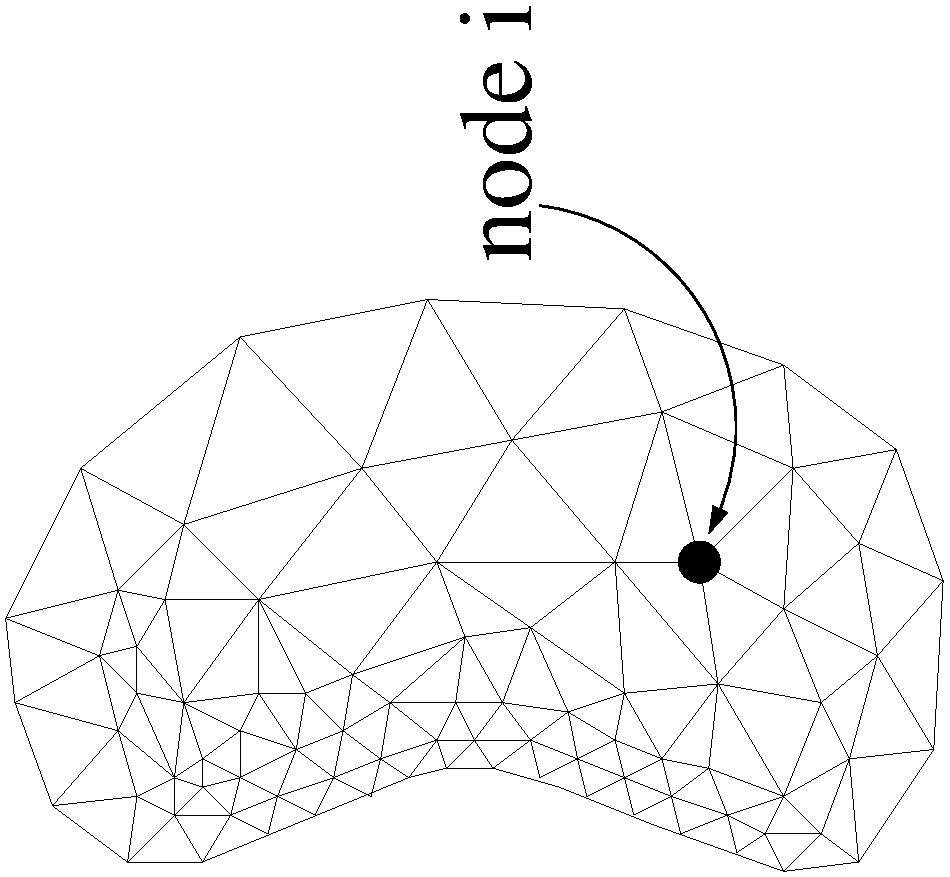
\includegraphics[width=2in,angle=-90]{figures/node_i}
%% 	    }
%% 	\only<2>
%% 	    {
%% 	      
\includegraphics[width=2in,angle=-90]{figures/phi_i}
%% 	    }
%% 	\only<3->
%% 	    {
	      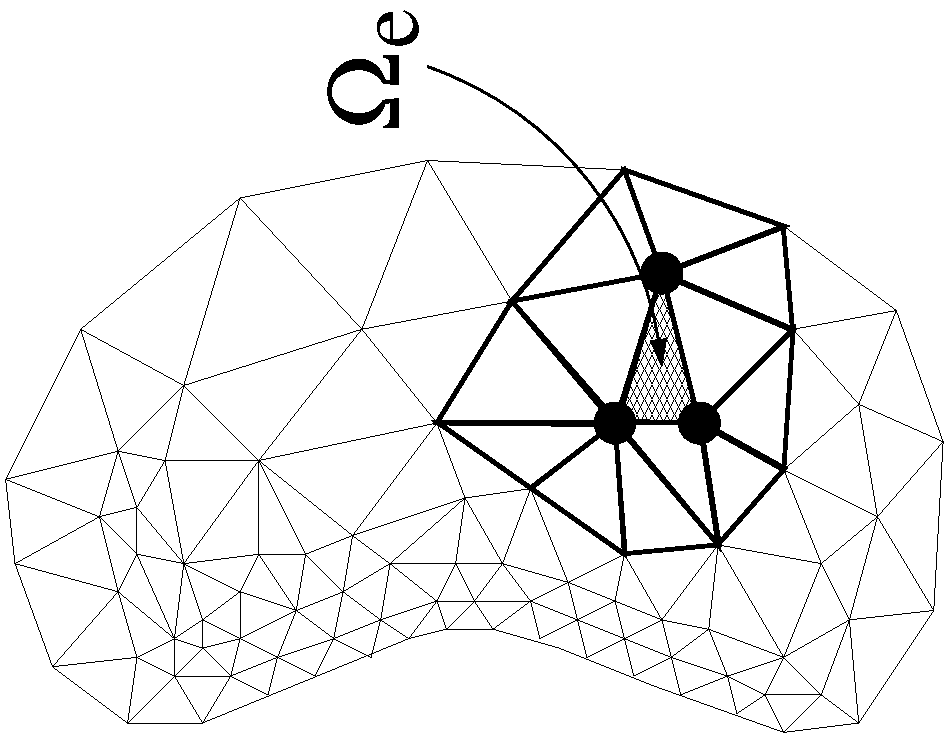
\includegraphics[width=2in,angle=-90]{figures/phi_ijk}
%%	    }
      \end{center}
    \end{columns}
\end{frame}
    
\subsection*{Element Matrix and Load Vector}
\begin{frame}%[t]
%  \frametitle{Poisson Equation}
  \begin{itemize}    
    \visible<1->
	{
	\item
	  {
	    The element integrals \ldots
	    \begin{equation}
	      \nonumber
	      \int_{\Omega_e} \left[ \nabla u^h \cdot \nabla v^h - fv^h \right] dx
	    \end{equation}
	  }
	}

	
      \visible<2->
      {
	\item{
	  are written in terms of the local ``$\alert<2>{\phi_i}$'' basis functions
	  \begin{equation}
	    \nonumber
		\alert<2>{\sum_{j=1}^{N_s}}  \alert<2>{u_j}   \int_{\Omega_e}
		\nabla \alert<2>{\phi_j} \cdot \nabla \alert<2>{\phi_i} \;dx
		- \int_{\Omega_e}  f\alert<2>{\phi_i} \;dx
		\hspace{.15in},\hspace{.15in} i = 1,\ldots,N_s
	  \end{equation}
	}
      }
      \visible<3>
      {
	\item{
	  This can be expressed naturally in matrix notation as
	\begin{equation}
	  \nonumber
	  \bv{K^e} \bv{U^e} - \bv{F^e} 
	\end{equation}
	}
      }
  \end{itemize}
 \end{frame}



%% \frame%[t]
%%     {
%%   \frametitle{Poisson Equation}
%%   \begin{itemize}    
%%   \item
%%     {
%%       \visible<1->
%%       {
%% 	The element integrals \ldots
%%       }
%%       \visible<2->
%%       {
%% 	are written in terms of the local ``$\alert<2>{\phi_i}$'' basis functions \ldots
%%       }
%%       \visible<3>
%%       {
%% 	which can be expressed naturally in matrix notation.
%% 	%element ``stiffness matrix'' $\alert{\bv{K_e}}$
%% 	%and ``load vector'' $\alert{\bv{F_e}}$. 
%%       }
%%     }
%%   \end{itemize}
%%     \begin{eqnarray}
%%       %\begin{center}
%% 	\nonumber
%% 	%\begin{array}{c}
%% 	\int_{\Omega_e} \left[ \nabla u^h \cdot \nabla v^h - fv^h \right] dx
%% 	\hspace{.75in} \\ \nonumber
%% 	  \visible<2->
%% 	      {
%% 		\Downarrow \hspace{1.5in} \\ \nonumber
%% 		%
%% 		\alert<2>{\sum_{j=1}^{N_s}}  \alert<2>{u_j}   \int_{\Omega_e}
%% 		\nabla \alert<2>{\phi_j} \cdot \nabla \alert<2>{\phi_i} \;dx
%% 		- \int_{\Omega_e}  f\alert<2>{\phi_i} \;dx
%% 		\hspace{.15in},\hspace{.15in} i = 1,\ldots,N_s \\ \nonumber
%% 	      }
%% 	      \visible<3>
%% 	      {\Downarrow \hspace{1.5in} \\ \nonumber
%% 		%
%% 		\bv{K_e} \bv{U_e} - \bv{F_e} \hspace{1.25in}
%% 	      }
%% 	%\end{array}
%%       %\end{center}
%%     \end{eqnarray}
%%     }

\subsection*{Global Linear System}
\begin{frame}%[<+->]
  %  \frametitle{Poisson Equation}
  \begin{itemize}
    \visible<1->{
    \item{
      The entries of the element stiffness matrix are the integrals
      \begin{equation}
	\nonumber
	\bv{K}^e_{ij} := 
	\int_{\Omega_e}
	\nabla \phi_j \cdot \nabla \phi_i \;dx
      \end{equation}
    }
    }
    \visible<2->{
    \item{ While for the element right-hand side we have 
      \begin{equation}
	\nonumber
	\bv{F}^e_{i} := 
	\int_{\Omega_e} f \phi_i \;dx
      \end{equation}
    }
    }
    \visible<3>{
    \item{ The element stiffness matrices and right-hand sides can be ``assembled'' to 
      obtain the global system of equations
      \begin{equation}
	\nonumber
	\bv{K} \bv{U} = \bv{F}
      \end{equation}    
    }
    }
  \end{itemize}
\end{frame}

\subsection*{Reference Element Map}


\begin{frame}[t]
%  \frametitle{Poisson Equation}
  \begin{block}{}
    \begin{itemize}    
  \item{
    The integrals are performed on a ``reference'' element $\alert<1>{\hat{\Omega}_e}$
    }
  \end{itemize}
  \end{block}
  %\vspace{-.3in}
  %\begin{center}   %Note: \centering is what makes the tables ``wiggle'' during slide transitions
  %% Three separate tabular elements.  The first column is an empty, fixed-width column designed
  %% to center the table without using centering commands.
    \only<1>
    {
    \begin{tabular}{p{.125\textwidth}ccc} \\
      &
      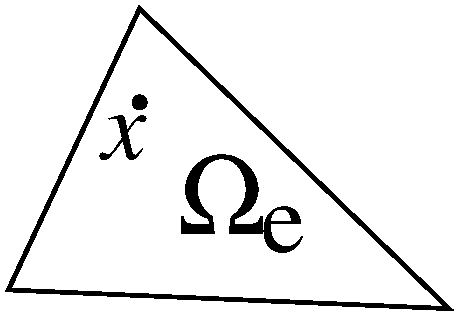
\includegraphics[width=.2\textwidth]{figures/physical_element}&
      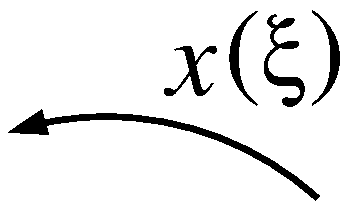
\includegraphics[width=.2\textwidth]{figures/map}&
      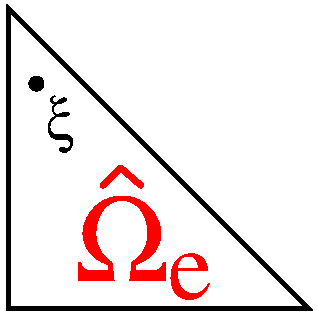
\includegraphics[width=.15\textwidth]{figures/reference_element_red}
    \end{tabular}
    }
    %
    \only<2>
    {
    \begin{tabular}{p{.125\textwidth}ccc} \\ 
      &
      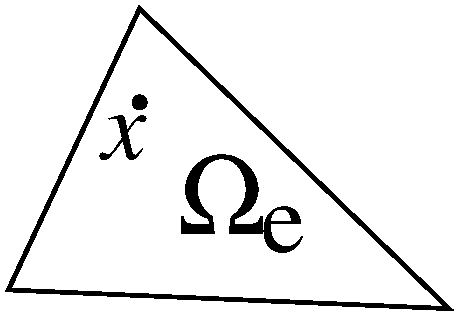
\includegraphics[width=.2\textwidth]{figures/physical_element}&
      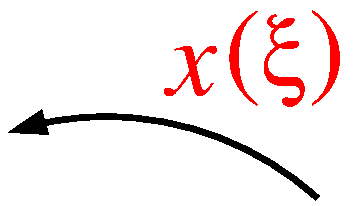
\includegraphics[width=.2\textwidth]{figures/map_red}&
      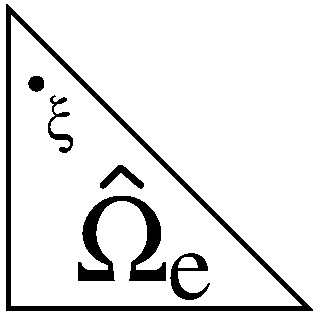
\includegraphics[width=.15\textwidth]{figures/reference_element}
    \end{tabular}
    }
    %
    \only<3>
    {
    \begin{tabular}{p{.125\textwidth}ccc} \\ 
      &
      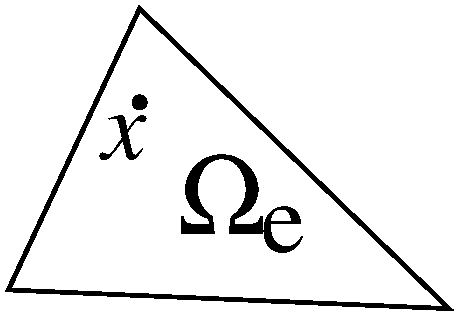
\includegraphics[width=.2\textwidth]{figures/physical_element}&
      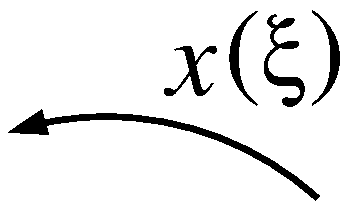
\includegraphics[width=.2\textwidth]{figures/map}&
      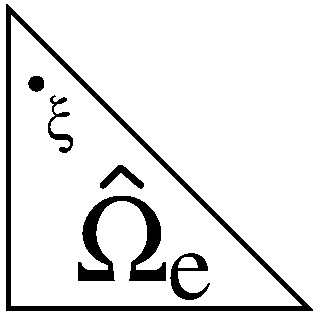
\includegraphics[width=.15\textwidth]{figures/reference_element}
    \end{tabular}
    }
    
%%     %% All in one table
%%     \begin{tabular}{ccc} \\ 
%%     %\fbox{
%%       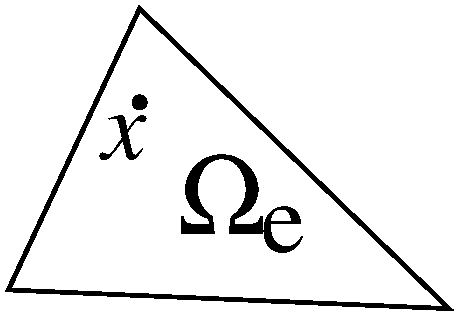
\includegraphics[width=.2\textwidth]{figures/physical_element}
%%     %}
%%        &
%%   \only<1,3->
%%   {
%%        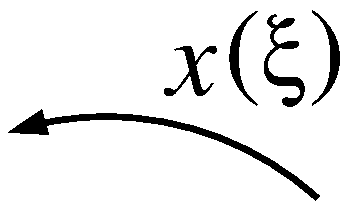
\includegraphics[width=.2\textwidth]{figures/map}
%%   }
%%   \only<2>
%%   {
%%        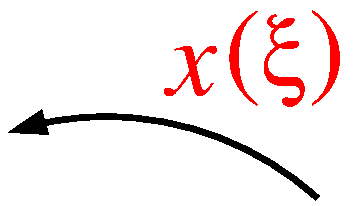
\includegraphics[width=.2\textwidth]{figures/map_red}
%%   }
%%        &
%%   \only<1>
%%   {
%%        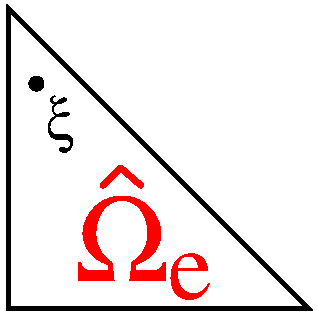
\includegraphics[width=.15\textwidth]{figures/reference_element_red}
%%        }
%%   \only<2->
%%   {
%%        \includegraphics[width=.15\textwidth]{figures/reference_element}
%%        }
%%      \end{tabular}
  %\end{center}


  \only<2>
      {
	\begin{block}{}
	\begin{itemize}    
	\item{
	  The Jacobian of the map $\alert{x(\xi)}$ is $\alert{J}$.
	}
	\end{itemize}
	\end{block}
	\begin{equation}
	  \nonumber
	  \bv{F}^e_{i} = \int_{\Omega_e} f \phi_i dx
	  =  \int_{\alert{\hat{\Omega}_e}}
	  f (\alert{x(\xi)}) \phi_i \alert{|J|} d\alert{\xi}
	\end{equation}
      }

\only<3>
{
  \begin{block}{}
  \begin{itemize}    
  \item{
    %The gradients are transformed
    Chain rule: 
    $\nabla 
    = J^{-1}\nabla_{\!\xi}
    := \alert{\hat{\nabla}_{\!\xi}}$
  }
  \end{itemize}
  \end{block}
  \begin{equation}
    \nonumber
    \bv{K}^e_{ij} =
    \int_{\Omega_e}
    \nabla \phi_j \cdot \nabla \phi_i \;dx =
    \int_{\hat{\Omega}_e}
    \alert{\hat{\nabla}_{\!\xi}} \phi_j \cdot
    \alert{\hat{\nabla}_{\!\xi}} \phi_i \;|J| d\xi
  \end{equation}
}
\end{frame}

\subsection*{Element Quadrature}
    
\begin{frame}[t]
%	\frametitle{Poisson Equation}
	\begin{block}{}
	\begin{itemize}    
	\item{
	  The integrals on the ``reference'' element are approximated via numerical
	  quadrature.
	}
	  \visible<2->
	      {
	      \item{The quadrature rule has $\alert{N_q}$ points
		``$\alert{\xi_q}$'' and weights ``$\alert{w_q}$''.}
	      }
	\end{itemize}
	\end{block}
\only<3>
{
	\begin{eqnarray}
	  \nonumber
%	  \only<3-4>
%	      {
		\bv{F}^e_{i} &=&
		\int_{\hat{\Omega}_e} f \phi_i |J| d\xi
		\\ \nonumber
%	      }
%	      \only<4>
%		  {
		    &\approx&
		    \alert{\sum_{q=1}^{N_q}}
		    f(x(\alert{\xi_q})) \phi_i(\alert{\xi_q})
		    |J(\alert{\xi_q})| \alert{w_q}
%		  }
	\end{eqnarray}
}

\only<4>
{
	\begin{eqnarray}
	  \nonumber
%	  \only<5-6>
%	      {
		\bv{K}^e_{ij} &=&
		\int_{\hat{\Omega}_e}
		\hat{\nabla}_{\!\xi}\phi_j \cdot
		\hat{\nabla}_{\!\xi}\phi_i \;|J| d\xi
		\\ \nonumber
%	      }
%	      \only<6>
%		  {
		    &\approx&
		    \alert{\sum_{q=1}^{N_q}}
		    \hat{\nabla}_{\!\xi} \phi_j(\alert{\xi_q}) \cdot
		    \hat{\nabla}_{\!\xi} \phi_i(\alert{\xi_q})
		    |J(\alert{\xi_q})| \alert{w_q}
%		  }
	\end{eqnarray}
}
\end{frame}

\subsection*{\texttt{LibMesh} Quadrature Point Data}
\begin{frame}[t]
%	\frametitle{Poisson Equation}
	\begin{block}{}
	\begin{itemize}    
	\item{ \texttt{LibMesh} provides the following variables at
	  each quadrature point $q$
	}
%% 	\item{``\texttt{JxW[q]}'' = $|J(\xi_q)| w_q$
%% 	  %the scalar value of the element Jacobian map times
%% 	  %the quadrature rule weight
%% 	}
	\end{itemize}
	\end{block}
	
	\begin{center}
	  \renewcommand{\arraystretch}{1.3}
	\begin{tabular}{|l|l|l|} \hline
	  \textbf{Code} & \textbf{Math} & \textbf{Description} \\ \hline
	  \texttt{JxW[q]}
	  & $|J(\xi_q)| w_q$
	  & Jacobian times weight
	  \\ \hline
	  \texttt{phi[i][q]}
	  & $\phi_i(\xi_{q})$
	  & value of $i^{th}$ shape fn.\
	  \\ \hline
	  \texttt{dphi[i][q]}
	  & $\hat{\nabla}_{\!\xi} \phi_i (\xi_q)$
	  & value of $i^{th}$ shape fn.\ gradient
	  \\ \hline
	  \texttt{xyz[q]}
	  & $x(\xi_q)$
	  & location of $\xi_q$ in physical space
	  \\ \hline
	  \end{tabular}
	\end{center}
	  
%      } %end frame
\end{frame}

\subsection*{Matrix Assembly Loops}
\begin{frame}[fragile,t]  
%  \frametitle{Poisson Equation}
	\begin{block}{}
	  \begin{itemize}    
	  \item{ The \libmesh{} representation of the matrix and
	    rhs assembly is similar to the mathematical statements.
	  }
	  \end{itemize}
	\end{block}
\small
\begin{semiverbatim}
for (q=0; q<Nq; ++q) 
  for (i=0; i<Ns; ++i) \{
    \alert<2>{Fe(i)   += \alert<3>{JxW[q]}*\alert<4>{f(xyz[q])}*\alert<5>{phi[i][q]};}
    
    for (j=0; j<Ns; ++j)
      \alert<6>{Ke(i,j) += \alert<7>{JxW[q]}*(\alert<8>{dphi[j][q]*dphi[i][q]});}
  \}
\end{semiverbatim}
\only<2-5>
{
  \begin{equation}
    \nonumber
    \bv{F}^e_{i} = 
    \sum_{q=1}^{N_q}
    \alert<4>{f(x(\xi_q))}
    \alert<5>{\phi_i(\xi_q)}
    \alert<3>{|J(\xi_q)| w_q}
  \end{equation}
}
\only<6->
{
  \begin{equation}
  \nonumber
  \bv{K}^e_{ij} =
  \sum_{q=1}^{N_q}
  \alert<8>{
    \hat{\nabla}_{\!\xi} \phi_j(\xi_q) \cdot
    \hat{\nabla}_{\!\xi} \phi_i(\xi_q)
    }
  \alert<7>{|J(\xi_q)| w_q}
  \end{equation}
}
\end{frame}


\begin{frame}[allowframebreaks]
  \lstinputlisting[basicstyle=\tiny\ttfamily]{snippets/poisson_eqn.cxx}
\end{frame}
 

\frame
{
  \Large
  \begin{block}{}
    \center{\bf A Complete Program:}
    \center{\texttt{poisson\_ex1}}
  \end{block}
}



\begin{frame}[fragile]
  \frametitle{Poisson class definition}

  \begin{lstlisting}
// headers omitted for brevity
class Poisson : public System::Assembly
{
public:
  Poisson (EquationSystems &es_in) :
    es (es_in)
  {}

  void assemble ();

  Real exact_solution (const Real x,
                       const Real y,
                       const Real z = 0.) const
  {
    static const Real pi = acos(-1.);

    return cos(.5*pi*x)*sin(.5*pi*y)*cos(.5*pi*z);
  }

private:
  EquationSystems &es;
};
  \end{lstlisting}
\end{frame}


\begin{frame}[allowframebreaks]
  \frametitle{Poisson \texttt{main()}}
  \lstinputlisting[basicstyle=\tiny\ttfamily]{tutorial/poisson_ex1/main.C}
\end{frame}


\begin{frame}[allowframebreaks]
  \frametitle{Poisson \texttt{main()}}
  \lstinputlisting[basicstyle=\tiny\ttfamily]{tutorial/poisson_ex1/poisson_problem.C}
\end{frame}


\begin{frame}[fragile]
  \frametitle{Running the program}
    \begin{block}{Running the program}
    \begin{lstlisting}[language=bash]
# copy the example

$ make

# run the example in 2D with 20 elements in each direction
$ ./example-opt -d 2 -n 20 

# run the example in 2D with 20 elements in each direction
$ ./example-opt -d 3 -n 20 
    \end{lstlisting}
  \end{block}
\end{frame}

\frame
{
  \frametitle{Output}
  \begin{center}
    \includegraphics[height=0.8\textheight]{tutorial/poisson_ex1/screen}
  \end{center}
} 

\frame
{
  \Large
  \begin{block}{}
    \center{\bf Extension: Multithreaded Assembly:}
    \center{\texttt{poisson\_threaded}}
  \end{block}
}



\begin{frame}[fragile,shrink]
  \frametitle{Poisson class definition}

  \begin{lstlisting}
// headers omitted for brevity
class Poisson : public System::Assembly
{
public:
  Poisson (EquationSystems &es_in) :
    es (es_in)
  {}

  void assemble ();

  void operator()(const ConstElemRange &range) const;

  Real exact_solution (const Real x,
                       const Real y,
                       const Real z = 0.) const
  {
    static const Real pi = acos(-1.);

    return cos(.5*pi*x)*sin(.5*pi*y)*cos(.5*pi*z);
  }

private:
  EquationSystems &es;

  mutable Threads::spin_mutex assembly_mutex;
};
  \end{lstlisting}
\end{frame}



\begin{frame}[fragile,shrink]
  \frametitle{Threaded Poisson assembly}

  \begin{lstlisting}
#include "poisson_problem.h"

void Poisson::assemble ()
{
  const MeshBase& mesh = es.get_mesh();

  ConstElemRange assembly_elem_range (mesh.active_local_elements_begin(),
                                      mesh.active_local_elements_end());

  Threads::parallel_for (// the range over which we will perform threaded operations
                         assembly_elem_range,

                         // the function object to apply to each element in the range
                         *this);
}

void Poisson::operator()(const ConstElemRange &range) const
{
  ...

  // insert the local (per-thread) element matrix/vector into
  // the global matrix/vector.  This is a shared object, so we
  // must be careful to lock for exclusive access.
  {
    Threads::spin_mutex::scoped_lock lock(assembly_mutex);
    
    system.matrix->add_matrix (Ke, dof_indices);
    system.rhs->add_vector    (Fe, dof_indices);
  }
}
  \end{lstlisting}
\end{frame}
\begin{frame}[fragile]
  \frametitle{Running the program}
    \begin{block}{Running the program}
    \begin{lstlisting}[language=bash]
# copy the example

$ make

# run the example in 2D with 20 elements in each direction
$ ./example-opt -d 2 -n 20 

# run the example in 2D with 20 elements in each direction
$ ./example-opt -d 3 -n 20 --n_threads=1
$ ./example-opt -d 3 -n 20 --n_threads=2
$ ./example-opt -d 3 -n 20 --n_threads=4

    \end{lstlisting}
  \end{block}
\end{frame}

      

\section{Other Examples}
% Auto-generate the TOC slide(s)
\begin{frame}
  \tableofcontents[currentsection]
  %\tableofcontents
\end{frame}



\subsection*{Convection-Diffusion Equation}
\begin{frame}[fragile]  
  \begin{block}{}
    \begin{itemize}    
    \item{The matrix assembly routine for the linear convection-diffusion equation,
      \begin{equation}
	\nonumber
	-\alert<2>{k}\Delta u + \alert<3>{\bv{b} \cdot \nabla u} = f
      \end{equation}
    }
    \end{itemize}
  \end{block}
  \small
  \begin{semiverbatim}
for (q=0; q<Nq; ++q) 
  for (i=0; i<Ns; ++i) \{
    Fe(i)   += JxW[q]*f(xyz[q])*phi[i][q];
    
    for (j=0; j<Ns; ++j)
      Ke(i,j) += JxW[q]*(\alert<2>{k}*(dphi[j][q]*dphi[i][q]) 
                       +(\alert<3>{b*dphi[j][q]})*phi[i][q]);
  \}
  \end{semiverbatim}
\end{frame}

\subsection*{Stokes Flow}
\begin{frame}[t]  
  \begin{block}{}
    \begin{itemize}    
    \item{For multi-variable systems like Stokes flow,
      \begin{equation}
	\begin{array}{rcl}
	  \nonumber
	  %\frac{\partial \bv{u}}{\partial t} +
	  %\left(\bv{u} \cdot \nabla\right) \bv{u} +
	  \nabla p - \nu \Delta \bv{u}  &=& \bv{f}
	  \\
	  \nonumber
	  \nabla \cdot \bv{u} &=& 0
	\end{array}  \hspace{.25in}  \in \hspace{.1in} \Omega \subset \mathbb{R}^2
      \end{equation}
    }
\vspace{-.25in}
      
    \item{The element stiffness matrix concept can extended to include sub-matrices
      \begin{eqnarray}
	\nonumber
	\label{eqn:Ke_stokes}
	\left[
	  \begin{array}{cc|c}
	    \alert<2>{K^e_{u_1 u_1}}   & K^e_{u_1 u_2}             &  K^e_{u_1 p}        \\
	    K^e_{u_2 u_1}              & \alert<3>{K^e_{u_2 u_2}}  &  K^e_{u_2 p} \\ \hline
	    K^e_{p u_1}                & \alert<4>{K^e_{p u_2}}    &  K^e_{p p}      \\
	  \end{array}
	  \right]
	\left[
  \begin{array}{c}
    U^e_{u_1} \\
    U^e_{u_2}\\ \hline
    U^e_{p}
  \end{array}
  \right]-
\left[
  \begin{array}{c}
    \alert<6>{F^e_{u_{1}}} \\
    \alert<7>{F^e_{u_{2}}} \\ \hline
    F^e_{p}
  \end{array}
  \right]
      \end{eqnarray}
    }


      \item
	{
	  \only<1-4>	      {We have an array of submatrices:}
	      \only<1>	      {\texttt{Ke[ ][ ]}}
	      \only<2>	      {\hspace{-0.05in}\texttt{Ke[\alert<2>{0}][\alert<2>{0}]}}
	      \only<3>	      {\hspace{-0.1in}\texttt{Ke[\alert<3>{1}][\alert<3>{1}]}}
	      \only<4>        {\hspace{-0.15in}\texttt{Ke[\alert<4>{2}][\alert<4>{1}]}}

      \only<5->          { 	  And an array of right-hand sides: }
 	\only<5> {\texttt{Fe[]}.}
	\only<6> {\hspace{-0.05in}\texttt{Fe[\alert{0}]}.}
	\only<7> {\hspace{-0.1in}\texttt{Fe[\alert{1}]}.}
	}

	
%%       \only<1>
%% 	  {
%% 	  \item{
%% 	    We have an array of submatrices
%% 	    \texttt{Ke[ ][ ]}.
%% 	  }
%% 	  }

%% 	  \only<2>
%% 	  {
%% 	  \item{
%% 	    We have an array of submatrices
%% 	    \texttt{Ke[\alert<2>{1}][\alert<2>{1}]}.
%% 	  }
%% 	  } 
%%           \only<3>
%%           {
%%  	  \item{
%%  	    In this case, we have an array of submatrices
%%  	    \texttt{Ke[\alert<3>{2}][\alert<3>{2}]}.
%%  	  }
%% 	  }
%%           \only<4>
%%           {
%%  	  \item{
%%  	    In this case, we have an array of submatrices
%%  	    \texttt{Ke[\alert<4>{3}][\alert<4>{2}]}.
%%  	  }
%% 	  }
%%           \only<5>
%%           {
%%  	  \item{
%%  	    And an array of right-hand sides
%%  	    \texttt{Fe[]}.
%%  	  }
%% 	  }
%% 	  \only<6>
%% 	  {
%%  	  \item{
%%  	    And an array of right-hand sides
%%  	    \texttt{Fe[\alert{1}]}.
%%  	  }
%% 	  }
    \end{itemize}
  \end{block}
\end{frame}




\begin{frame}[fragile] 
  \begin{block}{}
    \begin{itemize}    
    \item{The matrix assembly can proceed in essentially the same way.}
    \item{For the momentum equations:}
    \end{itemize}
  \end{block}
  \small
\begin{semiverbatim}
for (q=0; q<Nq; ++q) 
  \alert{for (d=0; d<2; ++d)}
    for (i=0; i<Ns; ++i) \{
      Fe\alert{[d]}(i) += JxW[q]*f(xyz[q],\alert{d})*phi[i][q];
      
      for (j=0; j<Ns; ++j)
        Ke\alert{[d][d]}(i,j) +=
	            JxW[q]*nu*(dphi[j][q]*dphi[i][q]);
    \}
\end{semiverbatim}
\end{frame}


\section{Essential BCs}
% Auto-generate the TOC slide(s)
\begin{frame}
  \tableofcontents[currentsection]
  %\tableofcontents
\end{frame}



\subsection*{Essential Boundary Data}
\begin{frame}[t]
  %\vspace{-.2in}
  \begin{block}{
      %Essential Boundary Data
    }
  \begin{itemize}
  \item {Dirichlet boundary conditions can be enforced after 
    the global stiffness matrix $\bv{K}$ has been assembled}
  \item This usually involves
    \begin{enumerate}
    \item<1-> placing a ``1'' on the main diagonal of the
      global stiffness matrix
    \item<2-> zeroing out the row entries
    \item<3-> placing the Dirichlet
      value in the rhs vector
    \item<4-> subtracting off the column entries from the rhs
    \end{enumerate}
  \end{itemize}
  \end{block}
  \visible<5->{
    \vspace{-0.1in}
  \begin{equation}
    \nonumber
      \begin{bmatrix}
	k_{11} & k_{12} & k_{13} & .  \\
	k_{21} & k_{22} & k_{23} & .  \\
	k_{31} & k_{32} & k_{33} & .  \\
	  .    &   .    &    .   & .  
      \end{bmatrix},
      \begin{bmatrix}
	f_{1}  \\
	f_{2}  \\
	f_{3}  \\
	  .     
      \end{bmatrix} \rightarrow
      \begin{bmatrix}
	1      & 0      & 0      & 0  \\
	0      & k_{22} & k_{23} & .  \\
	0      & k_{32} & k_{33} & .  \\
	  0    &   .    &    .   & .  
      \end{bmatrix},
      \begin{bmatrix}
	g_{1}  \\
	f_{2} - k_{21}g_1  \\
	f_{3} - k_{31}g_1  \\
	  .     
      \end{bmatrix}      
  \end{equation}}

\end{frame}



\begin{frame}[c]
%\begin{block}{}
  \begin{itemize}[<+->]
    \item {Cons of this approach :
      \begin{itemize}[<+->]
      \item {Works for an interpolary finite element basis
	but not in general.}
	
      \item {May be inefficient to change individual entries once the global matrix is assembled.}
      \end{itemize}
      }
    \item {Need to enforce boundary conditions for
      a generic finite element basis \emph{at the element stiffness matrix level}.}

    %\item Solution: ``Penalty'' Boundary Conditions
  \end{itemize}
%  \end{block}
\end{frame}


\subsection*{Penalty Formulation}
\begin{frame}[c]
%\begin{block}{}
  \begin{itemize}[<+->]
  \item {One solution is the ``penalty'' boundary formulation}
    %
  \item {A term is added to the standard weighted residual statement
    \begin{equation}
      \nonumber
      (F( u ), v)
      + \underbrace{\frac{1}{\epsilon} \int_{\partial \Omega_D} (u-u_D)v \; dx}_{\text{penalty term}} =
      0 \hspace{.3in} \forall v \in \mathcal{V}
    \end{equation}
  }
    %
  \item {Here $\epsilon \ll 1$ is chosen so that, in floating point arithmetic,
    $\frac{1}{\epsilon} + 1 = \frac{1}{\epsilon}$.}
    %
  \item {This weakly enforces $u=u_D$ on the Dirichlet boundary, and works for
    general finite element bases.}

%%   \item It requires a few additional calculations (edge/face integrals) but is more
%%     efficient than modifying row entries after assembly
  \end{itemize}
%  \end{block}
\end{frame}



\begin{frame}[fragile]
  \begin{block}{}
  \texttt{\libMesh{}} provides:
  \begin{itemize}
  \item {A quadrature rule with \texttt{Nqf} points and \texttt{JxW\_f[]}}
  \item {A finite element coincident with the boundary face that has % \texttt{Nf}
    shape function values \texttt{phi\_f[][]}}
  \end{itemize}
  \end{block}
\small
  \begin{semiverbatim}
for (qf=0; qf<Nqf; ++qf) \{
  for (i=0; i<Nf; ++i) \{
    Fe(i) += JxW_f[qf]*
      \alert<2>{penalty}*\alert<3>{uD(xyz[q])}*phi_f[i][qf];
	
    for (j=0; j<Nf; ++j)
      Ke(i,j) += JxW_f[qf]*
        \alert<2>{penalty}*phi_f[j][qf]*phi_f[i][qf];
  \}
\}
    \end{semiverbatim}

\end{frame}

%\section{Some Extensions}
% Auto-generate the TOC slide(s)
\begin{frame}
  \tableofcontents[currentsection]
  %\tableofcontents
\end{frame}



\subsection*{Time-Dependent Problems}
\begin{frame}%[t]
  \only<1>{
  }
%%   \begin{block}{}
%%     The weighted residual statement provides the connection between the mathematical
%%     statement of the problem and the computer code implementation of the problem:
%%   \end{block}

  %\begin{block}{}
  \begin{itemize}
    \only<1>
	{
	\item{For linear problems, we have already seen how
	  the weighted residual statement
	  leads directly to a sparse linear system of equations
	  \begin{equation}
	    \nonumber
	    \bv{K} \bv{U} = \bv{F}
	  \end{equation}
	  %which can be solved via Krylov subspace iterative methods.
	}
	}
    \only<2>
	{
	\item{For time-dependent problems, 
	  \begin{equation}
	    \nonumber
	    \frac{\partial u}{\partial t} = F(u)
	  \end{equation}
	}
	\item{we also need a way to advance the
	  solution in time, e.g. a $\theta$-method
	  \begin{eqnarray}
	    \nonumber
	    \left( \frac{ u^{n+1} - u^n}{\Delta t}, v^h\right) &=& \left(F(u_{\theta}), v^h\right)
	    \hspace{.1in} \forall v^h \in \mathcal{V}^h
	    %+ \mathcal{O}(\Delta t^{p(\theta)})
	    \\ \nonumber
	    u_{\theta} &:=& \theta u^{n+1} + (1-\theta)u^n
	  \end{eqnarray}
	\item{Leads to $\bv{K} \bv{U} = \bv{F}$ at \emph{each timestep}.}
	}
	}
  \end{itemize}
%\end{block}
\end{frame}





\subsection*{Nonlinear Problems}
\begin{frame}
  \begin{itemize}
	\item{For nonlinear problems, typically a sequence of linear problems must be solved, e.g.
	  for Newton's method
	  \begin{equation}
	    \nonumber
	    (F'( u^k ) \delta u^{k+1}, v) = -(F( u^k ), v) 
	  \end{equation}
	  where $F'( u^k )$ is the linearized (Jacobian) operator associated with
	  the PDE.	}

	\item{Must solve $\bv{K} \bv{U} = \bv{F}$ (Inexact Newton method) at \emph{each iteration step}.}
  \end{itemize}
\end{frame}


\frame
{
  \Large
  \begin{block}{}
    \center{\bf Examples: Nonlinear \& Transient Problems}
    \center{\texttt{laplace\_young}}
    \center{\texttt{transient\_convection\_diffusion}}
  \end{block}
}

\frame
{
  \frametitle{Lapace-Young ``minimal surface'' problem}

  The Laplace-Young equation governs the behavior of films, which seek to form a minimal surface:
  \begin{equation*}
    -\grad{}\cdot\left(\frac{\grad{u}}{\sqrt{1 + \grad{u}\cdot\grad{u}}}\right) + \kappa u = 0
  \end{equation*}
  or equivalently
  \begin{equation*}
    -\grad{}\cdot\left(K\left(u\right)\,\grad{u}\right) + \kappa u = 0
  \end{equation*}
  
  This problem behaves like a Helmholtz problem with nonlinear diffusion coefficient, $K(u)$.
}

\begin{frame}[fragile,shrink]
  \frametitle{Laplace-Young Assembly}
  \begin{lstlisting}
// headers omitted for brevity
class LaplaceYoung : public NonlinearImplicitSystem::ComputeJacobian,
                     public NonlinearImplicitSystem::ComputeResidual
{
public:  
  LaplaceYoung (EquationSystems &es_in) :
    es(es_in)
  {}

  virtual void jacobian (const NumericVector<Number>& X,
                         SparseMatrix<Number>& J,
                         NonlinearImplicitSystem& S);

  virtual void residual (const NumericVector<Number>& X,
                         NumericVector<Number>& R,
                         NonlinearImplicitSystem& S); 

private:
  EquationSystems &es;
};
  \end{lstlisting}
\end{frame}
\begin{frame}[fragile]
  \frametitle{Running the program}
    \begin{block}{Running the program}
    \begin{lstlisting}[language=bash]
# copy the example

$ make

# run the example with 3 uniform refinement steps, using first
# order Lagrange elements
$ ./example-opt -r 3 -o FIRST 

# run the example with 3 uniform refinement steps, using first
# order Lagrange elements
$ ./example-opt -r 3 -o SECOND
    \end{lstlisting}
  \end{block}
\end{frame}


\frame
{
  \frametitle{Output}
  \begin{center}
    \includegraphics[height=0.8\textheight]{tutorial/laplace_young/screen}
  \end{center}
} 


\frame
{
  \frametitle{Output}
  \begin{center}
    \includegraphics[height=0.8\textheight]{tutorial/transient_convection_diffusion/screen}
  \end{center}
} 
 
\section{Examples}
\subsection{Fluid Dynamics}
\begin{frame}%[<+=>]
  \frametitle{Introduction}
\small
  \begin{itemize}[<+->]
    \item Laplace-Young equation model surface tension effects for enclosed liquids.
    \item Combining surface tension, gravity and contact the energy functional for Laplace-Young is:
      \begin{gather*}
       % E(u,\nabla u)
       % =
        \int_\Omega \sqrt{1+|\nabla u|^2} \;d\Omega
        +
        \int_\Omega \frac 12 \kappa u^2 \;d\Omega
        -
        \int_{\partial\Omega} \sigma u \;ds
      \end{gather*}
      \item Where $\kappa$ is the ratio of surface energy to gravitational energy and $u$ is the height of the liquid.

    \item While the weak formulation of the stationary condition is given by:
      \begin{align}
        \label{eq:weak}
       % a(\kappa,\sigma;u,\varphi)
       % =
        \left(\frac{\nabla u}{\sqrt{1+|\nabla u|^2}},
          \nabla \varphi \right)_\Omega
        +
        \kappa\left(u,\varphi\right)_\Omega
        =
        \sigma \left(1,\varphi\right)_{\partial\Omega} 
%        \qquad
%        \forall \varphi\in V
      \end{align}

    \item By specifying the parameter $\sigma=cos(\gamma)$ (where $\gamma$ is the contact angle) along the boundary, the liquid height $u$ can be solved for.
  \end{itemize}
\end{frame}

\begin{frame}[fragile,t]
\tiny
\begin{block}{}
  Instead of explicitly finding the Jacobian, we'll use FEMSystem to finite difference the weak form.
\end{block}

\begin{block}{element\_constraint()}
\begin{semiverbatim}
  for (unsigned int qp=0; qp != n_qpoints; qp++) \{
    Number u = interior_value(0, qp);
    Gradient grad_u = interior_gradient(0, qp);
    \alert<2>{Number K = 1. / sqrt(1. + (grad_u * grad_u));}

    for (unsigned int i=0; i != n_u_dofs; i++) \{
      Fu(i) += JxW[qp] * ((\alert<5>{_kappa * u * phi[i][qp]}) +
               (\alert<2>{K} * \alert<3>{grad_u} * \alert<4>{dphi[i][qp]}));
    \}
  \}
\end{semiverbatim}
\end{block}

\begin{block}{side\_constraint()}
\begin{semiverbatim}
  for (unsigned int qp=0; qp != n_qpoints; qp++) \{
    for (unsigned int i=0; i != n_u_dofs; i++) \{
      Fu(i) -= JxW[qp] * \alert<6>{_gamma * phi[i][qp]};
    \}
  \}
\end{semiverbatim}
\end{block}

\begin{block}{}
   \begin{equation}
     \nonumber
       \left(\frac{\alert<3>{\nabla u}}{\alert<2>{\sqrt{1+|\nabla u|^2}}},
           \alert<4>{\nabla \varphi} \right)_\Omega
         +
         \alert<5>{\kappa\left(u,\varphi\right)_\Omega}
         -
         \alert<6>{\sigma \left(1,\varphi\right)_{\partial\Omega}} 
         =
         0
         \qquad
         \forall \varphi\in V
   \end{equation}
\end{block}

\end{frame}

\frame
{
  \frametitle{Solution}
  \small
  \begin{itemize}[<+->]
    \item An overkill solution containing 200,000 DOFs.
  \end{itemize}
      \begin{figure}[!htb]
        \begin{center}
          \subfigure[2D.]{\label{fig:ly_over_2d}\includegraphics[viewport=40 20 660 650,clip=true,width=.42\textwidth]{figs/ly_over_2d}}
          \subfigure[Contour Elevation.]{\label{fig:ly_over_3d}\includegraphics[viewport=50 70 620 550,clip=true,width=.42\textwidth]{figs/ly_over_3d}}
        \label{fig:ly_over}
        \end{center}
      \end{figure}
}

% \frame
% {
%   \frametitle{Redistributed Solution}
%   \begin{itemize}[<+->]
%     \item Using a set of variational smoothing functionals and an error indicator for redistribution the following grid and solution can be obtained.
%       \begin{figure}[!htb]
%         \begin{center}
%           \subfigure[Mesh.]{\label{fig:ly_redist_11_mesh}\includegraphics[viewport=110 30 600 550,clip=true,width=.42\textwidth]{figs/ly_redist_14_mesh.pdf}}
%           \subfigure[Solution.]{\label{fig:ly_redist_11_sol}\includegraphics[viewport=110 30 600 520,clip=true,width=.42\textwidth]{figs/ly_redist_14_sol.pdf}}
%           \label{fig:ly_over}
%         \end{center}
%       \end{figure}
%   \end{itemize}
% }

\subsection*{Compressible Flow}

\frame
{
  \frametitle{Compressible Shocked Flow}
  \begin{itemize}[<+->]
    \item Original compressible flow code written by Ben Kirk utilizing libMesh.
      \begin{itemize}[<+->]
      \item Solves both Compressible Navier Stokes and Inviscid Euler.
      \item Includes both SUPG and a shock capturing scheme.
      \end{itemize}
    \item Original redistribution code written by Larisa Branets.
      \begin{itemize}[<+->]
      \item Simultaneous optimization of element shape and size.
      \item Directable via user supplied error estimate.
      \end{itemize}
    \item Integration work done by Derek Gaston.
      \begin{itemize}[<+->]
      \item Combination of redistribution, $h$ refinement.
      \item Applicable to other problem classes.
      \end{itemize}
  \end{itemize}
}

\frame
{
  \frametitle{Problem Specification}
  \begin{itemize}[<+->]
    \item The problem studied is that of an oblique shock generated by a $10^o$ wedge angle. 
      \begin{itemize}[<+->]
      \item This problem has an exact solution for density which is a step function.
      \item Utilizing libmesh's exact solution capability the exact
$L_2$ error can be solved for.
      \item The exact solution is shown below:
        \begin{figure}
          \begin{center}
            \includegraphics[viewport=20 10 660 600,clip=true,width=.4\textwidth]{shock.pdf}
          \end{center}
        \end{figure}
    \end{itemize}
  \end{itemize}
}

\frame
{
  \frametitle{Uniformly Refined Solutions}
  \begin{itemize}[<+->]
  \item For comparison purposes, here is a mesh and a solution after 1 uniform refinement with 10890 DOFs.
    \begin{figure}[!htb]
      \begin{center}
        \subfigure[Mesh after 1 uniform refinement.]{\label{fig:fob_uniform_2_mesh}\includegraphics[viewport=110 30 600 550,clip=true,width=.42\textwidth]{fob_uniform_2_mesh.pdf}}
        \subfigure[Solution after 1 uniform refinement.]{\label{fig:fob_uniform_2_sol}\includegraphics[viewport=110 30 600 520,clip=true,width=.42\textwidth]{fob_uniform_2_sol.pdf}}
      \end{center}
    \end{figure}
  \end{itemize}
}

\frame
{
  \frametitle{H-Adapted Solutions}
  \begin{itemize}[<+->]
    \item A flux jump indicator was employed as the error indcator along with a statistical flagging scheme.
    \item Here is a mesh and solution after 2 adaptive refinements containing 10800 DOFs:
      \begin{figure}[!htb]
        \begin{center}
          \subfigure[Mesh, 2 refinements]{\label{fig:fob_adapt_3_mesh}\includegraphics[viewport=110 30 600 550,clip=true,width=.42\textwidth]{fob_adapt_3_mesh.pdf}}
          \subfigure[Solution]{\label{fig:fob_adapt_3_sol}\includegraphics[viewport=110 30 600 520,clip=true,width=.42\textwidth]{fob_adapt_3_sol.pdf}}
        \end{center}
      \end{figure}
  \end{itemize}
}

\frame
{
  \frametitle{Redistributed Solutions}
  \begin{itemize}[<+->]
    \item Redistribution utilizing the same flux jump indicator.
      \begin{figure}[!htb]
        \begin{center}
          \subfigure[Mesh, 8 redistribution steps]{\label{fig:fob_redist_adapt_8_mesh}\includegraphics[viewport=110 30 600 550,clip=true,width=.42\textwidth]{fob_redist_adapt_8_mesh.pdf}}
          \subfigure[Solution]{\label{fig:fob_redist_adapt_8_sol}\includegraphics[viewport=110 30 600 520,clip=true,width=.42\textwidth]{fob_redist_adapt_8_sol.pdf}}
        \end{center}
      \end{figure}
  \end{itemize}
}

\frame
{
  \frametitle{Redistributed and Adapted}
  \begin{itemize}[<+->]
    \item Now combining the two, here are the mesh and solution after 2 adaptations beyond the previous redistribution containing 10190 DOFs.
      \begin{figure}[!htb]
        \begin{center}
          \subfigure[Mesh, 2 refinements]{\label{fig:fob_redist_adapt_10_mesh}\includegraphics[viewport=110 30 600 550,clip=true,width=.42\textwidth]{fob_redist_adapt_10_mesh.pdf}}
          \subfigure[Solution]{\label{fig:fob_redist_adapt_10_sol}\includegraphics[viewport=110 30 600 520,clip=true,width=.42\textwidth]{fob_redist_adapt_10_sol.pdf}}
        \end{center}
      \end{figure}
  \end{itemize}
}

\frame
{
  \frametitle{Solution Comparison}
  \begin{itemize}[<+->]
    \item For a better comparison here are 3 of the solutions, each with around 11000 DOFs:
      \begin{figure}[!htb]
        \begin{center}
          \subfigure[Uniform.]{\label{fig:fob_uniform_2_sol}\includegraphics[viewport=110 30 600 520,clip=true,width=.3\textwidth]{fob_uniform_2_sol.pdf}}
          \subfigure[Adaptive.]{\label{fig:fob_adapt_3_sol}\includegraphics[viewport=110 30 600 520,clip=true,width=.3\textwidth]{fob_adapt_3_sol.pdf}}
          \subfigure[R + H.]{\label{fig:fob_redist_adapt_10_sol}\includegraphics[viewport=110 30 600 520,clip=true,width=.3\textwidth]{fob_redist_adapt_10_sol.pdf}}
        \end{center}
      \end{figure}
  \end{itemize}
}

\frame
{
  \frametitle{Error Plot}
  \begin{itemize}[<+->]
    \item libmesh provides capability for computing error norms against an exact solution.
    \item The exact solution is not in $H^1$ therefore we only obtain
the $L_2$ convergence plot:
      \begin{figure}[!htb]
      \begin{center}
        \subfigure[LogLog plot of L2 vs DOFs.]{\label{fig:fob_l2}\includegraphics[viewport=0 10 600 400,clip=true,width=.7\textwidth]{fob_l2.pdf}}
      \end{center}
      \end{figure}
  \end{itemize}
}

\frame
{
  %\frametitle{Other Compressible Flow Examples}
    \begin{figure}[!htb]
      \begin{center}
        \subfigure{\label{fig:fob_uniform_2_sol}\includegraphics[width=.4\textwidth]{Hypersonic_cow_mach}}
        \subfigure{\label{fig:fob_adapt_3_sol}\includegraphics[width=.4\textwidth]{Benkirk_orbiter_reentry_side_view}}
        \subfigure{\label{fig:fob_redist_adapt_10_sol}\includegraphics[width=.4\textwidth]{Benkirk_schlieren}}
        \subfigure{\label{fig:fob_redist_adapt_10_sol}\includegraphics[width=.4\textwidth]{Benkirk_double_cone_M}}
      \end{center}
    \end{figure}
}

\subsection*{Natural Convection}
\begin{frame}[t]
  \begin{center}
    \includegraphics[width=.45\textwidth]{part_trans}
    %\\
    \includegraphics[width=.45\textwidth]{streamtraces}
  \end{center}
  \begin{block}{}
    \begin{itemize}
    \item{
      Tetrahedral mesh of ``pipe'' geometry.
      Stream ribbons colored by temperature.
      }
      \end{itemize}
  \end{block}
\end{frame}

\begin{frame}[t]
  \frametitle{Surface-Tension-Driven Flow}
  \begin{center}
    \includegraphics[width=.6\textwidth]{figs/rbm_adapt_soln}    
  \end{center}

  \begin{block}{}
    \begin{itemize}
    \item{Adaptive grid solution shown
      with temperature contours and velocity vectors.
      }
      \end{itemize}
  \end{block}
\end{frame}

\begin{frame}[t]
  \frametitle{Double-Diffusive Convection}
  \begin{center}
    \includegraphics[width=.6\textwidth]{figs/dd}    
  \end{center}

  \begin{block}{}
    \begin{itemize}
    \item{Solute contours: a plume of
      warm, low-salinity fluid is convected upward through a porous medium.
      }
      \end{itemize}
  \end{block}
\end{frame}



\subsection{Biology}
\subsection*{Tumor Angiogenesis}
\begin{frame}[t]
  \begin{center}
    \includegraphics[width=.6\textwidth]{tumor_model}    
  \end{center}

  \begin{block}{}
    \begin{itemize}
    \item{%Tumor angiogenesis model simulation.
      The tumor secretes
      a chemical which stimulates blood vessel formation.
      }
      \end{itemize}
  \end{block}
\end{frame}



%\section{Macroelement Spaces}

%%%%%%%%%%%%%%%%%%%%%%%%%%%%%%%%%%%%%%%%%%%%%%%%%%%%%%%%%%%%%%%%%%%%%
\royslide{$C^1$ Finite Element Spaces}{
In Galerkin formulations of plate bending, streamfunction viscous
flow, Cahn-Hilliard interfaces, and surface
tension driven films, we find integrated products
of second derivatives of the solution and test functions.

With variational problems posed on subspaces of $H^2(\Omega)$,
conforming finite element approximations
require $H^2$ conforming functions.

A $C^1$ continuous (and $W^{2,\inf}$ bounded, $W^{2,p}$ conforming)
finite element is needed, e.g.:

\royitemizebegin
	\item Powell-Sabin 6-split triangle
	\item Powell-Sabin-Heindl (PSH) 12-split triangle
	\item Hsieh-Clough-Tocher (HCT) 3-split triangle
\royitemizeend
}



%%%%%%%%%%%%%%%%%%%%%%%%%%%%%%%%%%%%%%%%%%%%%%%%%%%%%%%%%%%%%%%%%%%%%
\royslide{Macroelements}{

Constraining polynomial triangles to $C^1$ continuity
requires quintic polynomials.  To use lower $p$,
we construct macroelements by
subdividing each triangle, using piecewise polynomial functions
with continuity constraints along interior edges.

\begin{center}
\fbox{\includegraphics[width=.9\textwidth]{figs/triangles}}
\end{center}

% Mention additional ``raw'' degrees of freedom

% Mention spectral methods

}



%%%%%%%%%%%%%%%%%%%%%%%%%%%%%%%%%%%%%%%%%%%%%%%%%%%%%%%%%%%%%%%%%%%%%
%\royslide{Constructing Macroelements}{
%
%To reliably construct a macroelement basis:
%
%\begin{itemize}
%\item Number the ``raw'' degrees of freedom
%\item ``Write'' all constraints as matrix rows
%\item Put constraint matrix in row reduced form
%\item Add boundary DoF equations (checking each for
%linear independence)
%\item If necessary, make matrix square with interior DOF
%equations (again checking for linear independence)
%\item Invert matrix, multiply by $\hat{e}_i$ to get basis coefficients
%corresponding to the DOF on row $i$
%\end{itemize}
%
%}


%%%%%%%%%%%%%%%%%%%%%%%%%%%%%%%%%%%%%%%%%%%%%%%%%%%%%%%%%%%%%%%%%%%%%
%\royslide{Powell-Sabin 6-split}{
%\begin{center}
%\fbox{\includegraphics[width=.7\textwidth]{figs/Basis_psrt}}
%\end{center}
%}


%\royslide{Powell-Sabin-Heindl 12-split}{
%\begin{center}
%\fbox{\includegraphics[width=.7\textwidth]{figs/Basis_hrt}}
%\end{center}
%}


%\royslide{Clough-Tocher 3-split}{
%\begin{center}
%\fbox{\includegraphics[width=.7\textwidth]{figs/Basis_ctrt}}
%\end{center}
%}


%%%%%%%%%%%%%%%%%%%%%%%%%%%%%%%%%%%%%%%%%%%%%%%%%%%%%%%%%%%%%%%%%%%%%
\royslide{Approximation Convergence}{
PSH and HCT triangles exactly
reproduce quadratics and cubics $(k \equiv 2, 3)$,
respectively.  Standard interpolation, $H^2$ approximation rules
apply for $w \in H^n(\Omega) \subset H^{k+1}(\Omega)$, but $L_2$
approximation on PSH triangles is suboptimal.

\begin{eqnarray*}
%P_h(f) & \equiv & \sum_{i=1}^{N} \sigma_i(f)\phi_i \\
\norm{w - P_h w}_{H^m(\Omega)}
& \leq & C h^{n-m} \abs{w}_{H^n(\Omega)} \\
%\norm{u - u_h}_{H^2(\Omega)} & \leq & \left( 1 + \frac{\norm{B}}{\alpha_h} \right)
\norm{u - u_h}_{H^2(\Omega)} & \leq & 
C h^{n-2} \norm{u}_{H^n(\Omega)} \\
\norm{u - u_h}_{H^r(\Omega)} & \leq & 
C h^{\min \left(2(k+1-m),k+1-r,n-r\right)} \norm{u}_{H^n(\Omega)}
\end{eqnarray*}
}


%%%%%%%%%%%%%%%%%%%%%%%%%%%%%%%%%%%%%%%%%%%%%%%%%%%%%%%%%%%%%%%%%%%%%
%\royslide{$H^2$ Approximation Convergence}{
%
%Given that our operator is bounded and satisfies an inf-sup
%condition on our $H^2$ conforming function space $P$, Galerkin
%orthogonality (the C\'{e}a lemma) gives us the expected (linear for
%Powell-Sabin, quadratic for Clough-Tocher) asymptotic error in the
%$H^2$ norm, for problems with sufficiently smooth (contained in
%$H^n(\Omega)$, for $n \equiv k + 1$) solutions:
%
%\vspace{-2em}
%\begin{eqnarray*}
%\alpha_h & \equiv & \inf_{v_h \in P} \sup_{w_h \in P}
%\frac{B(v_h,w_h)}{\norm{v_h}_P \norm{w_h}_P} \\
%\norm{u - u_h}_{H^2(\Omega)} & \leq & \left( 1 + \frac{\norm{B}}{\alpha_h} \right)
%\inf_{v_h \in P} \norm{u - v_h}_{H^2(\Omega)} \\
%& \leq & \left( 1 + \frac{\norm{B}}{\alpha_h} \right)
%\norm{u - P_h u}_{H^2(\Omega)} \\
%& \leq & \left( 1 + \frac{\norm{B}}{\alpha_h} \right)
%C h^{n-2} \abs{u}_{H^n(\Omega)} \\
%\end{eqnarray*}
%\vspace{-2em}
%
%}


%%%%%%%%%%%%%%%%%%%%%%%%%%%%%%%%%%%%%%%%%%%%%%%%%%%%%%%%%%%%%%%%%%%%%
%\royslide{$L_2$ Approximation Convergence}{
%
%HCT elements obtain an additional power of $h$ in $H^2$
%convergence.
%The difference grows in the $L_2$
%norm.  Defining $\eta \equiv \min \left(2(k+1-m),k+1-r,n-r\right)$,
%if $u_h$ is the Galerkin approximation to a bilinear problem on
%$H^m(\Omega)$,
%
%\begin{eqnarray*}
%\norm{u - u_h}_{H^r(\Omega)} \leq C h^{\eta} \norm{u}_{H^n(\Omega)}
%\end{eqnarray*}
%
%For $k = 3$, or $k = 2, r \geq 1$, this is the standard rule
%of thumb.
%
%For fourth order problems ($m = 2$), quadratic elements ($k = 2$), and
%the $L_2$ norm ($r = 0$), the $\eta \leq 2(k+1-m)$ term dominates.
%}

%\section{General AMR/C}


%%%%%%%%%%%%%%%%%%%%%%%%%%%%%%%%%%%%%%%%%%%%%%%%%%%%%%%%%%%%%%%%%%%%%
\royslide{Adaptive $h$ Constraints}{

Constraining hanging degrees of freedom can be more difficult on
general non-hierarchic bases

\begin{minipage}[h]{.45\textwidth}
  \begin{figure}[h]
    \begin{center}
      \includegraphics[width=.5\textwidth]{figs/adaptive}
    \end{center}
  \end{figure}
\end{minipage}
\begin{minipage}[h]{.45\textwidth}
\begin{eqnarray*}
u^F & = & u^C \\
\sum_i u_i^F \phi_i^F & = & \sum_j u_j^C \phi_j^C \\
A_{ki} u_i & = & B_{kj} u_j \\
u_i & = & A_{ki}^{-1} B_{kj} u_j
\end{eqnarray*}
\end{minipage}

Integrated values (and fluxes, for $C^1$ continuity) give
element-independent matrices:
\begin{eqnarray*}
A_{ki} & \equiv & (\phi_i^F, \phi_k^F) \\
B_{kj} & \equiv & (\phi_j^C, \phi_k^F)
\end{eqnarray*}

}


%%%%%%%%%%%%%%%%%%%%%%%%%%%%%%%%%%%%%%%%%%%%%%%%%%%%%%%%%%%%%%%%%%%%%
\royslide{Adaptive $p$ Constraints}{

\begin{minipage}[h]{.45\textwidth}
\begin{center}
\includegraphics[width=.9\textwidth]{figs/PHierarchic}
\end{center}
\end{minipage}
\begin{minipage}[h]{.45\textwidth}
\royitemizebegin
\item $p$ refinement is well suited to hierarchic adaptivity
\item Hanging degree of freedom coefficients are simply set to 0
\royitemizeend
\end{minipage}
}


%%%%%%%%%%%%%%%%%%%%%%%%%%%%%%%%%%%%%%%%%%%%%%%%%%%%%%%%%%%%%%%%%%%%%
\royslide{Error Indicators}{

Integration by parts gives an upper error bound on subelements $S$ for
the biharmonic problem:

\begin{eqnarray*}
   \norm{e}_{H^2(\Omega)} & \leq & C_\Omega
   \sum_S \left[\norm{f - \Delta^2 u_h}_S h_S^{2} + \right. \\
& & \left.
   \frac{1}{2} \norm{\jump{\dn{\Delta u_h}}}_{\partial S} h_S^{3/2} +
   \frac{1}{2} \norm{\jump{\Delta u_h}}_{\partial S} h_S^{1/2} \right]
\end{eqnarray*}

The most significant term gives a simple indicator on elements $K$ for
more general fourth order problems:

\[ \eta_K \equiv \sqrt{h_K} \norm{\jump{\Delta u_h}}_{\partial K}
\]

}



%%%%%%%%%%%%%%%%%%%%%%%%%%%%%%%%%%%%%%%%%%%%%%%%%%%%%%%%%%%%%%%%%%%%%
\royslide{Diffuse Interface Modeling with AMR/C}{

\begin{minipage}[h]{.45\textwidth}
\begin{center}
\includegraphics[width=.9\textwidth]{figs/cross-adaptive}
\end{center}
\end{minipage}
\begin{minipage}[h]{.45\textwidth}
\royitemizebegin
\item Mesh coarsening in smooth regions is traded for mesh
refinement in sharp layers
\item Equivalent accuracy is achieved here with 75\% fewer degrees of
freedom than a uniform mesh
\royitemizeend
\end{minipage}

}



%%%%%%%%%%%%%%%%%%%%%%%%%%%%%%%%%%%%%%%%%%%%%%%%%%%%%%%%%%%%%%%%%%%%%
\royslide{Diffuse Interface Modeling with AMR/C}{

\begin{minipage}[h]{.45\textwidth}
\begin{center}
\includegraphics[width=.9\textwidth]{figs/spinodal-adaptive}
\end{center}
\end{minipage}
\begin{minipage}[h]{.45\textwidth}
\royitemizebegin
\item Adaptive Mesh Refinement / Coarsening reduces solver expense
\item Laplacian Jump error indicator tracks moving interfaces
\royitemizeend
\end{minipage}

}



%%%%%%%%%%%%%%%%%%%%%%%%%%%%%%%%%%%%%%%%%%%%%%%%%%%%%%%%%%%%%%%%%%%%%
\royslide{Adaptive Refinement Strategies}{

Maintaining a constant global error estimate:
\royitemizebegin
\item Tracks time-varying complexity
\item Gives reliable results
\item Requires reliable error bounds
\royitemizeend

Maintaining constant element count:
\royitemizebegin
\item Keeps an upper bound on computational expense
\item Only requires a good feature indicator
\royitemizeend

}

\subsection{Material Science}
%%%%%%%%%%%%%%%%%%%%%%%%%%%%%%%%%%%%%%%%%%%%%%%%%%%%%%%%%%%%%%%%%%%%%
\royslide{Free Energy Formulation}{

Cahn-Hilliard systems model phase separation and interface
evolution

\begin{eqnarray*}
f(c, \nabla c) & \equiv & f_0(c) + f_\gamma(\nabla c) \\
f_\gamma(\nabla c) & \equiv & \frac{\epsilon_c^2}{2} \nabla c \cdot \nabla c \\
%f_{0m}(c) & \equiv & \frac{1}{4} \left( c^2 - 1 \right)^2 \\
f_0(c) & \equiv & N k T \left( c \ln{(c)} + 
(1-c) \ln{(1-c)} \right) + 
N \omega c (1-c)
\end{eqnarray*}

\begin{eqnarray*}
\dt{c} & = & \nabla \cdot M_c \nabla
  \left( f_0'(c) - \epsilon_c^2 \Laplacian c \right)
\end{eqnarray*}
}


\subsection{Cahn-Hilliard Simulations}

%%%%%%%%%%%%%%%%%%%%%%%%%%%%%%%%%%%%%%%%%%%%%%%%%%%%%%%%%%%%%%%%%%%%%
\royslide{Mesh Refinement}{

\begin{minipage}[h]{.45\textwidth}
\begin{center}
\includegraphics[width=.9\textwidth]{figs/chem-0250}
\end{center}
\end{minipage}
\begin{minipage}[h]{.45\textwidth}
\royitemizebegin{Coarse mesh}
\item $32 \times 32$ bicubic elements
\item $\Delta t = 2.500 \times 10^{-4}$
\item $t = 0.0625$
\item Mesh resolution must capture equilibrium interface width
\item Timesteps are limited by nonlinear solver
\royitemizeend
\end{minipage}

}


%%%%%%%%%%%%%%%%%%%%%%%%%%%%%%%%%%%%%%%%%%%%%%%%%%%%%%%%%%%%%%%%%%%%%
\royslide{Mesh Refinement}{

\begin{minipage}[h]{.45\textwidth}
\begin{center}
\includegraphics[width=.9\textwidth]{figs/chem-0500}
\end{center}
\end{minipage}
\begin{minipage}[h]{.45\textwidth}
\royitemizebegin{One Refinement}
\item $64 \times 64$ bicubic elements
\item $\Delta t = 1.250 \times 10^{-4}$
\item $t = 0.0625$
\item Free energy decay limits most error growth
\item Primary exception: interface topology changes
\royitemizeend
\end{minipage}

}

%%%%%%%%%%%%%%%%%%%%%%%%%%%%%%%%%%%%%%%%%%%%%%%%%%%%%%%%%%%%%%%%%%%%%
\royslide{Mesh Refinement}{

\begin{minipage}[h]{.45\textwidth}
\begin{center}
\includegraphics[width=.9\textwidth]{figs/chem-1000}
\end{center}
\end{minipage}
\begin{minipage}[h]{.45\textwidth}
\royitemizebegin{Two Refinements}
\item $128 \times 128$ bicubic elements
\item $\Delta t = 0.625 \times 10^{-4}$
\item $t = 0.0625$
\item Finite Element error becomes negligible
\item Uncertainty issues remain
\royitemizeend
\end{minipage}

}

%%%%%%%%%%%%%%%%%%%%%%%%%%%%%%%%%%%%%%%%%%%%%%%%%%%%%%%%%%%%%%%%%%%%%
\royslide{Mesh Refinement}{

\begin{minipage}[h]{.55\textwidth}
\begin{center}
\includegraphics[width=.9\textwidth]{figs/cherror}
\end{center}
\end{minipage}
\begin{minipage}[h]{.4\textwidth}
\royitemizebegin{Transient Error}
\item With layers well-resolved, error remains bounded
\royitemizeend
\end{minipage}

}



%%%%%%%%%%%%%%%%%%%%%%%%%%%%%%%%%%%%%%%%%%%%%%%%%%%%%%%%%%%%%%%%%%%%%
\royslide{Adaptive Time Stepping}{

\begin{columns}
\begin{column}{.55\textwidth}
\begin{center}
\includegraphics[width=.9\textwidth]{figs/adaptivetimesteps}
\end{center}
\end{column}
\begin{column}{.45\textwidth}
\royitemizebegin{}
\item CahnHilliardSystem
\item Euler2Solver
\item AdaptiveTimeSolver
\item Orders of magnitude speedup
\royitemizeend
\end{column}
\end{columns}

}



%%%%%%%%%%%%%%%%%%%%%%%%%%%%%%%%%%%%%%%%%%%%%%%%%%%%%%%%%%%%%%%%%%%%%
\royslide{Phase Separation - Spinodal Decomposition}{

\royitemizebegin{Initial Evolution}
\item Initial homogeneous blend quenched below critical T
\item Random perturbations rapidly segregate
into two distinct phases, divided by a labyrinth of sharp interfaces
\item Rapid anti-diffusionary process
\royitemizeend

\begin{center}
\includegraphics[width=.3\textwidth]{figs/ch3D02-006}
\includegraphics[width=.3\textwidth]{figs/ch3D02-012}
\includegraphics[width=.3\textwidth]{figs/ch3D02-024}
%\includegraphics[width=.3\textwidth]{figs/ch010}
%\includegraphics[width=.3\textwidth]{figs/ch050}
%\includegraphics[width=.3\textwidth]{figs/ch100}
\end{center}
}


%%%%%%%%%%%%%%%%%%%%%%%%%%%%%%%%%%%%%%%%%%%%%%%%%%%%%%%%%%%%%%%%%%%%%
\royslide{Phase Separation - Interfacial Flow}{

\royitemizebegin{Long-term Evolution}
\item Single-phase regions gradually coalesce
\item Motion into curvature vector resembles surface tension
\item Patterning may occur when additional stress, surface tropisms
are applied
\royitemizeend

\begin{center}
\includegraphics[width=.3\textwidth]{figs/ch3D02-048}
\includegraphics[width=.3\textwidth]{figs/ch3D02-096}
\includegraphics[width=.3\textwidth]{figs/ch3D02-192}
%\includegraphics[width=.3\textwidth]{figs/ch100}
%\includegraphics[width=.3\textwidth]{figs/ch200}
%\includegraphics[width=.3\textwidth]{figs/ch500}
\end{center}

}


%\section{References}

%%%%%%%%%%%%%%%%%%%%%%%%%%%%%%%%%%%%%%%%%%%%%%%%%%%%%%%%%%%%%%%%%%%%%
\royslide{References}{

B. Kirk, J. Peterson, R. Stogner and G. Carey, ``libMesh: a C++
library for parallel adaptive mesh refinement/coarsening
simulations'', \textit{Engineering with Computers} 2006;
\textbf{70}(9):237--254

\vspace{.5cm}

R. Stogner and G. Carey, ``$C^1$ macroelements in adaptive finite
element methods'', \textit{Int. J. Num. Meth. Eng.} 2007;
\textbf{70}(9):1076--1095

\vspace{.5cm}

R. Stogner, B. Murray, and G. Carey, ``Approximation of
Cahn-Hilliard diffuse interface models using parallel adaptive mesh
refinement and coarsening with $C^1$ elements'', \textit{Int. J. Num.
Meth. Eng.}, in press
}



%%%%%%%%%%%%%%%%%%%%%%%%%%%%%%%%%%%%%%%%%%%%%%%%%%%%%%%%%%%%%%%%%%%%%
%\royslide{Ongoing Work}{
%
%\begin{itemize}
%\item Application specific error estimates
%\item Application specific a posteriori estimators
%\item Further validation experiments
%\item Flow phenomena studies
%\end{itemize}
%
%R. Stogner, B. Murray, and G. Carey, ``Approximation of Cahn-Hilliard
%systems in $C^1$ finite element spaces'', in progress
%
%}


\end{document}




